% =====================================================================
%  Memoria de título — Plataforma web para la gestión integral y
%  asistencia de diseño en estudios de tatuaje
%  Pablo Nicolás Correa Mella — Universidad de Talca
%
%  Reconstruido a partir de Correa_Pablo_2021407028.pdf (Memoria Avance 2).
%  Compilar con pdfLaTeX + Biber:
%      pdflatex main && biber main && pdflatex main && pdflatex main
%  (En Overleaf basta con «Recompilar»: detecta Biber solo.)
%
%  Las imágenes van en la carpeta imagenes/ con los nombres que se usan en
%  cada \includegraphics (la lista completa está en imagenes/LEEME.txt).
% =====================================================================
\documentclass[12pt,letterpaper,oneside]{report}

% ---------- Idioma y codificación ----------
% Sin fontenc: el original usa las fuentes Computer Modern clásicas (OT1).
\usepackage[utf8]{inputenc}
\usepackage[spanish,es-tabla]{babel}
\usepackage{csquotes}

% ---------- Página ----------
\usepackage[left=4cm,right=2.5cm,top=4cm,bottom=2.5cm,
            headheight=12pt,headsep=59.4pt,footskip=30pt]{geometry}
\usepackage{setspace}
\onehalfspacing
\setlength{\parskip}{2mm plus 2pt}

% ---------- Matemática, figuras y tablas ----------
\usepackage{amsmath,amssymb}
\usepackage{graphicx}
\usepackage{float}
\graphicspath{{imagenes/}}
\usepackage{caption}
\usepackage{longtable}
\setlength{\LTpost}{7.12pt plus 4pt minus 4pt}
\usepackage{booktabs}
\usepackage{array}

% ---------- Títulos ----------
\usepackage{titlesec}
\titleformat{\chapter}[hang]
  {\normalfont\Huge\bfseries}{\thechapter.}{\dimexpr1.5em+2pt\relax}{}[\vspace{8.7pt}{\titlerule[2pt]}]
\titleformat{name=\chapter,numberless}[hang]
  {\normalfont\Huge\bfseries}{}{0pt}{}
\titlespacing*{\chapter}{0pt}{65.44pt}{29.92pt}
\titlespacing*{name=\chapter,numberless}{0pt}{65.95pt}{31pt}
% Secciones y subsecciones con el mecanismo estándar de LaTeX (no titlesec):
% así el espacio antes del título se combina con el que deja una lista igual
% que en el original.
\makeatletter
\renewcommand\section{\@startsection{section}{1}{\z@}%
  {-12.37pt \@plus -1ex \@minus -.2ex}{6.20pt \@plus.2ex}{\normalfont\large\bfseries}}
\renewcommand\subsection{\@startsection{subsection}{2}{\z@}%
  {-11.11pt\@plus -1ex \@minus -.2ex}{2.06pt \@plus .2ex}{\normalfont\normalsize\bfseries}}
\renewcommand\subsubsection{\@startsection{subsubsection}{3}{\z@}%
  {-11.11pt\@plus -1ex \@minus -.2ex}{2.06pt \@plus .2ex}{\normalfont\normalsize\bfseries}}
\makeatother

% Listas: espaciado medido sobre el original. El nivel es la profundidad total
% (una lista de viñetas dentro de una numerada es de nivel 2). Las listas de
% descripción (glosario) se quedan con la definición estándar de LaTeX.
\let\descripcionlatex\description
\let\enddescripcionlatex\enddescription
\usepackage{enumitem}
\setlist[1]{topsep=4.31pt plus 4pt minus 6pt,partopsep=3pt plus 2pt minus 2pt}
\setlist[2]{topsep=4.96pt plus 2.5pt minus 1pt}
\let\description\descripcionlatex
\let\enddescription\enddescripcionlatex

% ---------- Bibliografía ----------
\usepackage[backend=biber,style=numeric,sorting=none]{biblatex}
\addbibresource{bibliografia.bib}
% La bibliografía empieza más arriba que los demás capítulos sin número.
\defbibheading{bibintoc}[\bibname]{%
  {\titlespacing*{name=\chapter,numberless}{0pt}{44.38pt}{31pt}\chapter*{#1}}%
  \addcontentsline{toc}{chapter}{#1}\markboth{\MakeUppercase{#1}}{\MakeUppercase{#1}}}

% ---------- Enlaces (invisibles al imprimir, como en el original) ----------
\usepackage[hidelinks]{hyperref}

% ---------- Encabezados de las páginas preliminares ----------
% «AGRADECIMIENTOS», «RESUMEN», etc.: centrados, en negrita y del tamaño del texto.
\newcommand{\titulopreliminar}[1]{%
  \begin{center}\textbf{#1}\end{center}}

% Tabla de contenidos e índices con el rótulo «página» sobre los números.
\makeatletter
% Los índices van sin espacio entre párrafos (solo el texto lo lleva).
% En los índices de figuras y tablas el espacio que deja el primer capítulo se
% absorbe en el del rótulo (\vskip en vez de \vspace), como en el original.
\newcommand{\rotulopagina}[1]{\par\vspace{-5.69pt}\hfill página\par#1}
\newcommand{\indice}[3]{%
  \titulopreliminar{#1}\rotulopagina{#3}{\setlength{\parskip}{0pt}\@starttoc{#2}}}
\renewcommand{\tableofcontents}{\indice{TABLA DE CONTENIDOS}{toc}{\vspace{13pt}}}
\renewcommand{\listoffigures}{\indice{ÍNDICE DE FIGURAS}{lof}{\vskip13pt}}
\renewcommand{\listoftables}{\indice{ÍNDICE DE TABLAS}{lot}{\vskip13pt}}
\makeatother

% Títulos de párrafo en negrita y con sangría («Historias de usuario»,
% «Inicio de iteración», …). La versión «pegada» no deja espacio con el texto.
\newcommand{\titulopar}[1]{\par\textbf{#1}\par}
\newcommand{\tituloparpegado}[1]{\par\textbf{#1}\\\indent\ignorespaces}

% =====================================================================
\begin{document}

% ---------- Portadas ----------
% Cada línea va en su coordenada medida sobre el original: \posy{y} convierte
% la distancia desde el borde superior de la hoja (en pt) a la coordenada del
% entorno picture, cuyo origen queda en la primera línea base del área de texto.
\newcommand{\centrox}{214.65}
\newcommand{\izqx}{17.6}
\newcommand{\posy}[1]{\fpeval{\origenportada-(#1)}}
\newcommand{\origenportada}{125.4}
\newcommand{\linea}[2]{\put(\izqx,\posy{#1}){\makebox(0,0)[bl]{#2}}}
\newenvironment{portada}{%
  \begin{titlepage}\setlength{\unitlength}{1pt}\noindent\begin{picture}(0,0)% Encabezado común de las dos portadas: logo, universidad, título y autor.
% Cada elemento va en su posición exacta (en pt, medida desde el borde
% superior del área de texto; X desde el margen izquierdo). Se usa dentro del
% entorno picture que abre \portada en main.tex.
\put(\fpeval{\centrox-1.25},\posy{71.0}){\makebox(0,0)[t]{
\includegraphics[width=2.2cm]{utalca1}}}
\put(\centrox,\posy{178.94}){\makebox(0,0)[b]{\large\textbf{UNIVERSIDAD DE TALCA}}}
\put(\centrox,\posy{196.94}){\makebox(0,0)[b]{\large FACULTAD DE INGENIERÍA}}
\put(\centrox,\posy{214.93}){\makebox(0,0)[b]{\large ESCUELA DE INGENIERÍA CIVIL EN COMPUTACIÓN}}
\put(\centrox,\posy{292.78}){\makebox(0,0)[b]{\Large\textbf{Plataforma web para la gestión integral y}}}
\put(\centrox,\posy{314.78}){\makebox(0,0)[b]{\Large\textbf{asistencia de diseño en estudios de tatuaje}}}
\put(\centrox,\posy{365.02}){\makebox(0,0)[b]{\textbf{PABLO NICOLÁS CORREA MELLA}}}
}%
  {\end{picture}\end{titlepage}}

\begin{portada}
  \linea{598.76}{Profesor Guía: FRANCISCO ARIAS}
  \linea{660.92}{Memoria para optar al título de}
  \linea{675.42}{Ingeniero Civil en Computación}
  \linea{708.93}{Curicó -- Chile}
  \linea{725.75}{mes: Mayo, año: 2026}
\end{portada}

% ---------- Portada con profesores informantes ----------
\begin{portada}
  \linea{489.43}{Profesor Guía: FRANCISCO ARIAS}
  \linea{515.93}{Profesor Informante:}
  \linea{542.44}{Profesor Informante:}
  \linea{604.60}{Memoria para optar al título de}
  \linea{619.09}{Ingeniero Civil en Computación}
  \linea{642.93}{El presente documento fue calificado con nota: \rule{1.755cm}{0.4pt}}
  \linea{699.43}{Curicó -- Chile}
  \linea{725.75}{mes: Mayo, año: 2026}
\end{portada}

% ---------- Páginas preliminares (números romanos en versalitas) ----------
\pagestyle{headings}
\renewcommand{\thepage}{\roman{page}}

\thispagestyle{plain}
\addcontentsline{toc}{chapter}{Dedicatoria}
\vspace*{\fill}
\begin{flushright}
  \textit{Dedicado a ...}
\end{flushright}
\vspace*{167.03pt}
\newpage

\thispagestyle{plain}
\addcontentsline{toc}{chapter}{Agradecimientos}
\titulopreliminar{AGRADECIMIENTOS}
\vspace{10.75pt}

Agradecimientos ...
\newpage

\thispagestyle{plain}
\addcontentsline{toc}{chapter}{Tabla de Contenidos}
\tableofcontents
\newpage

\thispagestyle{plain}
\addcontentsline{toc}{chapter}{Índice de Figuras}
\listoffigures
\newpage

\thispagestyle{plain}
\addcontentsline{toc}{chapter}{Índice de Tablas}
\listoftables
\newpage

\thispagestyle{plain}
\addcontentsline{toc}{chapter}{Resumen}
\titulopreliminar{RESUMEN}
\vspace{10.75pt}

En la actualidad, el flujo de trabajo de los tatuadores presenta una alta fragmentación tecnológica, lo que hace hace que los profesionales dividan sus tareas administativas y artísticas en múltiples sistemas no integados. La falta de herramientas unificadas genera ineficiencias a la hora de trabajar, ya sea adecuando el tatuaje en una zona establecida del cuerpo, en pérdidas de tiempo en el cálculo de presupuestos y problemas gestionando las citas con los clientes.

El proyecto propone el diseño y construcción de una plataforma web integral que unifica el flujo de trabajo del estudio de tatuajes. El sistema incorpora módulos de almacenamiento en la nube para bocetos, previsualización 3D sobre modelos anatómicos, gestión de inventario con cotizaciones automatizadas, y un agendador de citas integrando una API de mensajería para los recordatorios.

Desde un análisis crítico, la solución posee factibilidad técnica, operativa y económica. Al utilizar tecnologías web y librerías de código abierto, el sistema elimina la dependencia de licencias costosas y no requiere hardware especializado. También teniendo en cuenta que se cuenta con la ayuda de un tatuador experto que ayuda en el proceso de captura de requerimientos y pruebas del sistema en cada iteración a través de su retroalimentación.

Como proyección de impacto, es un producto mínimo viable (MVP) que optimiza el modelo de negocio, con un objetivo de disminución de ausentismo de clientes, reducción de tiempo administrativo en cálculos de costos e inventario y una disminución de tiempo invertido en pruebas de diseño sobre la piel.

\newpage

% ---------- Cuerpo: la numeración sigue la cuenta, ahora en arábigos ----------
\renewcommand{\thepage}{\arabic{page}}

\chapter{Introducción}

La digitalización y el desarrollo de software han comenzado a transformar el funcionamiento de las disciplinas creativas, abriendo nuevas oportunidades de optimización para el rubro del arte corporal. El diseño e implementación de plataformas a la medida permite a los artistas modernos modernizar sus flujos de trabajo tradicionales, logrando un equilibrio eficiente entre la gestión administrativa del estudio y la ejecución de su obra.\\
\indent El presente capítulo tiene como propósito describir las bases que fundamentan el trabajo realizado en esta memoria de título. Para ello, se expone inicialmente el contexto de crecimiento del rubro del tatuaje, seguido de la descripción detallada de la problemática detectada a nivel operativo y administrativo. Posteriormente, se define la propuesta de solución tecnológica, sus objetivos, los alcances que delimitan el desarrollo y, finalmente, el plan de trabajo estructurado para su ejecución.

\section{Contexto}

El presente marco teórico establece los fundamentos históricos, comerciales y socioculturales que respaldan el desarrollo de la plataforma. Para comprender la envergadura y necesidad de este proyecto, es necesario analizar la evolución del rubro del tatuaje, partiendo desde sus orígenes hasta consolidarse como una industria global, para luego conectar estas métricas en la realidad nacional y local.

El tatuaje forma parte de la historia del ser humano, siendo la evidencia más antigua el hallazgo de los restos momificados del cazador neolítico conocido como ``Ötzi'', datados hace más de 5.300 años. En civilizaciones antiguas, como la egipcia, romana y maya, la inserción de pigmentos bajo la epidermis cumplía funciones estrictamente identitarias, indicando estatus o linaje, y en otros casos, marcando a prisioneros y esclavos \cite{ballen2015}. Si bien durante gran parte de la historia occidental moderna el tatuaje estuvo estigmatizado y relegado a la criminalidad, a partir del siglo XX y XXI ha experimentado una resignificación profunda. En la actualidad, ha superado el estigma social para consolidarse como una expresión artística legítima y un medio de afirmación de la identidad y la subjetividad personal \cite{poulsen2021}.

En la actualidad, la industria del arte corporal es uno de los mercados de más rápido y constante crecimiento en el mundo. Según estimaciones globales, la industria alcanzó un valor aproximado de 2.420 millones de dólares en el año 2025, y se proyecta que ascienda a 6.220 millones de dólares para el año 2035, exhibiendo una Tasa de Crecimiento Anual Compuesta (CAGR) del 9,9 \% \cite{ide2026}. Este crecimiento exponencial está directamente impulsado por la creciente aceptación social de las modificaciones corporales, el cambio demográfico liderado por las generaciones ``Millennials'' y ``Gen Z'', y un mayor poder adquisitivo destinado a la autoexpresión \cite{ide2026}.

Esta tendencia global también se encuentra en el panorama chileno. Un estudio estadístico realizado por la consultora GfK Adimark evidenció que el 17 \% de los chilenos mayores de 15 años posee al menos un tatuaje. Dicha cifra experimenta un alza dramática al observar el segmento de adultos jóvenes (entre 25 y 34 años), donde el 38 \% de la población se encuentra tatuada. En la última década, la demanda en el país ha crecido de manera exponencial, posicionando el nivel técnico y artístico del tatuaje en Chile a la par de los mercados europeos y norteamericanos\cite{sepulveda2017}.

En un contexto local, la ciudad de Curicó no ha quedado ajena a esta explosión de demanda. El aumento sostenido de clientes ha propiciado la apertura de nuevos estudios y el establecimiento de artistas independientes en la zona que buscan ganarse un puesto en el mercado local. Por consiguiente, el desarrollo de este proyecto cobra una relevancia para el apoyo a este dinamismo local. Al dotar a los artistas de Curicó con herramientas tecnológicas, se busca potenciar su capacidad y facilitar su consolidación en un mercado en plena expansión.

\subsection{Descripción del problema}

Actualmente el trabajo de los tatuadores se encuentra muy fragmentando por las diferentes herramientas tecnológicas que se pueden utilizar al momento de realizar su trabajo, ya sea en el ámbito operativo como en lo artístico. El hecho de dividir sus labores crea dificultades para optimizar sus tareas de una forma limpia.

A continuación se detallan las problemáticas operativas y administrativas, las cuales fueron analizadas y planteadas por el señor Héctor Salazar Moya quien es un tatuador profesional de Curicó, que ha trabajado en el área durante varios años y en distintos estudios de tatuajes, por lo que tiene un conocimiento profundo de las dificultades que enfrentan los tatuadores de la actualidad.

En el ámbito operativo, uno de los mayores problemas es la previsualización del tatuaje en una zona concreta del cuerpo. Actualmente para visualizar como quedaría un boceto de un tatuaje se ocupa un elemento llamado ``stencil'', que es una guía en papel hectográfico que transfiere el diseño del papel a la piel del boceto original. El problema surge que este papel es un material que se desecha una vez utilizado, esto quiere decir que si el tatuador se equivoca en la posición que coloca el stencil tendría que repetirse de nuevo el proceso y ocupar material extra. Incluso muchas veces son los mismos clientes que cambian de opinión con respecto a la posición que les gustaría tener su tatuaje, y el hecho de que el tatuador pueda previsualizar el boceto en cualquier parte del cuerpo que considere el lugar más apropiado, le facilitaría sus decisiones artísticas y no tendría los problemas antes mencionados.

Con respecto al ámbito admnistrativo, es posible mencionar más problemáticas que viven los tatuadores para la gestión de su negocio. Para comenzar el agendamiento de las citas es uno de los principales problemas, debido a que no existe una herramienta dedicada para los tatuadores, lo que hace que la gestión de citas sea poco personalizable y haya problemas en la estructuración de tiempos del profesional. En relación a las citas, también hay problemas con los recordatorios hacia los clientes, debido a que muchos de ellos no se presentan a la hora adecuada o simplemente se olvidan de su cita el día acordado, debido a que es el tatuador el que tiene que recordar a sus clientes de forma manual el día antes de la sesión, por lo que al tener múltiples clientes esta acción se puede ver afectada por parte del tatuador.

Otro de los problemas es analizar correctamente el coste los tatuajes, si bien este precio se ve influnciado gran parte por el valor que le quiera dar el artista, analizar su costo real a partir de los materiales utilizados y el tiempo invertido en las sesiones es una labor que es dificil tenerla presente en todo momento.

Por último hay que mencionar también el problema con respecto a la gestión del inventario ya que surgen inconvenientes al momento de gastar insumos y no tener las nociones de cuanto material se va utilizando en cada sesión de trabajo y calcular también su reposición.

\begin{figure}[h]
  \centering
  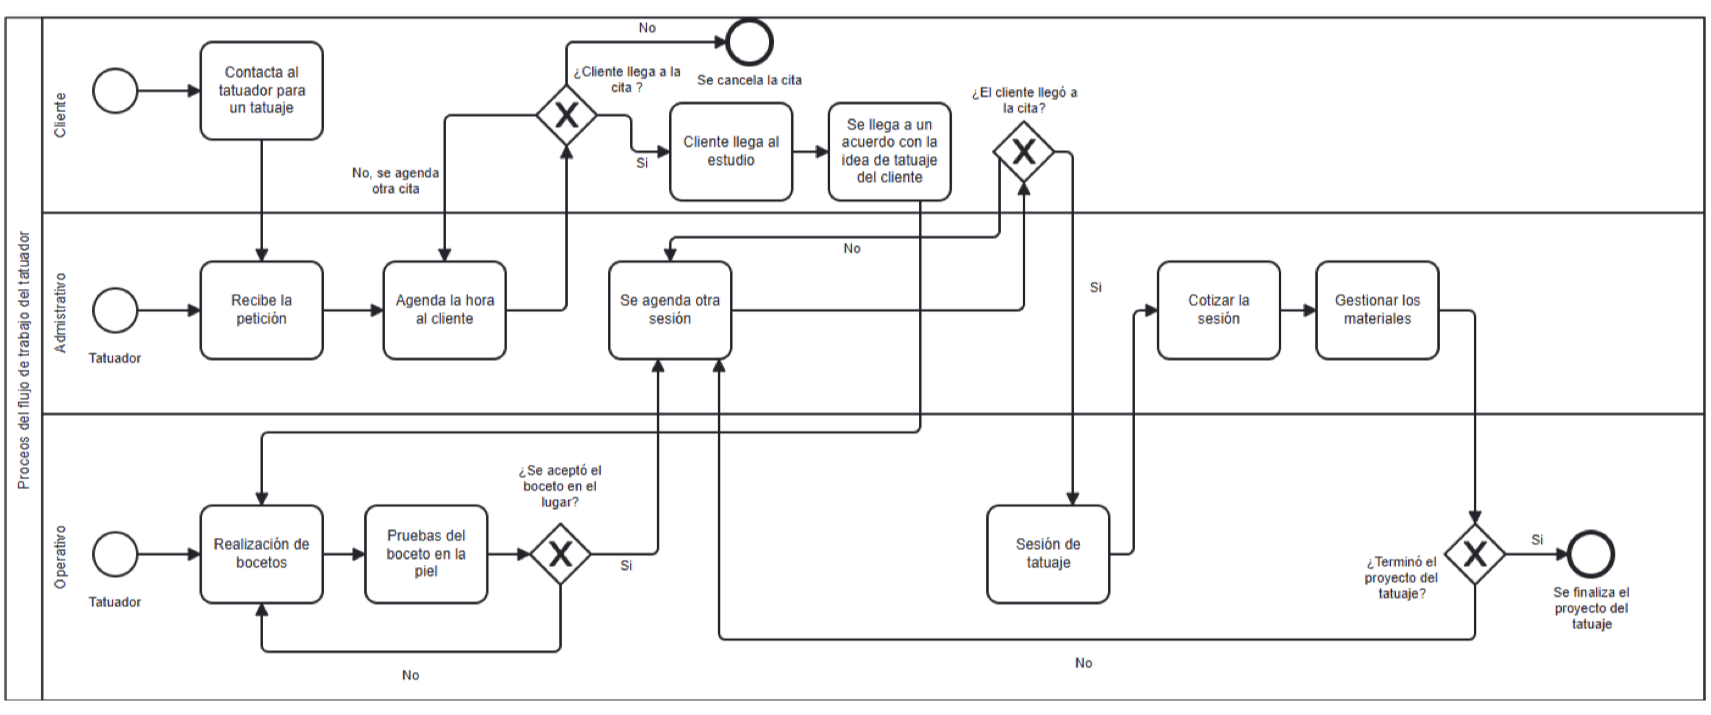
\includegraphics[width=\textwidth]{fig-1-1-bpmn}
  \caption[Modelo del proceso de negocio de un estudio de tatuajes (BPMN)]{Modelo del proceso de negocio de un estudio de tatuajes (BPMN)\cite{white2004}.}
  \label{fig:bpmn}
\end{figure}

La Figura \ref{fig:bpmn} representa el flujo del trabajo del tatuador, incluyendo su participación con el cliente, sus labores operativas y admistrativas. Esto describe la complejidad que conlleva desarrollar un proyecto de tatuaje con múltiples iteraciones, ya que, además de ser un proceso extenso, puede involucrar múltiples retrasos por parte del cliente al no poseer un recordatorio automatizado. Por otro lado los procesos que se integran en el trabajo son desarrollados en diferentes herramientas tanto admistrativamente como operativamente, lo que retrasa aún más este flujo.

\subsection{Propuesta de solución }

La solución propuesta consiste en el diseño y construcción de una plataforma web/móvil que unifique el flujo del trabajo de los artistas dedicados al arte del tatuaje, varias de sus funciones fueron creadas a partir de los requisitos de tatuador experto. El sistema considera distintos módulos como la importación y almacenamiento en la nube para la gestión de bocetos, la previsualización 3D sobre modelos anatómicos, el agendamiento de citas con recordatorios para reducir la inasistencia y retrasos de los clientes, un gestor de cotizaciones automatizadas y gestión de inventario.

Con respecto al módulo de importación y almacenamiento en la nube, este permite subir imágenes de los bocetos a la plataforma donde serán guardadas y visibles en la galería de la aplicación. Adicionalmente, el módulo contempla la generación de un enlace público asociado a la galería del tatuador, el cual puede ser compartido con clientes u otras personas interesadas para que visualicen el portafolio de diseños disponibles sin necesidad de contar con una cuenta en la plataforma.

En cuanto al módulo de previsualización 3D sobre modelos anatómicos, este permite visualizar un modelo 3D de un cuerpo humano en la plataforma gracias a un motor de renderizado, en donde los bocetos subidos son transformados para adherirse a la superficie 3D del cuerpo y desplazarse para encontrar la posición y el ángulo que el cliente prefiera.

Sobre el módulo de agendamientos de citas con recordatorios, este permite hacer agendas personalizadas, en donde se puede crear las citas a partir de los nombres de las personas a atender, en las cuales para cada perfil se puede crear una nueva sesión de tatuaje o un nuevo proyecto, donde se pueden incluir la hora de la cita, el precio de la sesión o proyecto, junto con una foto del proceso del tatuaje. Para el problema de los recordatorios se propone implementar una API que integra los mensajes de WhatsApp\cite{whatsapp}, donde se vinculan los números para enviar avisos antes y despues de la sesión del tatuaje.

El módulo de gestión de cotizaciones automatizadas, permite calcular el precio aproximado del costo del tatuaje a partir del boceto subido a la plataforma, esto se realiza mediante un algoritmo que procesa las dimensiones del boceto, junto con otros parámetros como el grosor de los trazados y colores, ya que el costo se centra en los gastos de material como agujas, tinta y otros insumos para la elaboración del tatuaje, dejando de lado valor adicional que le quiera dar el artista de acuerdo a la complejidad del diseño.

Por último, el módulo de gestión de inventario se encarga de gestionar los materiales que posea el tatuador, ya sea agujas, tintas, insumos de higiene, entre otros, los que puede a editar a su disposición y a la vez se pueden actualizar automaticamente cada vez que se haga una cotización automatizada.

En términos de factibilidad, esta solución es viable gracias a varios factores en los que incluye factibilidad técnica, operativa y económica. En el ámbito técnico, la solución se apoya en las tecnologías orientadas al desarrollo web, empleando librerías de código abierto establecidas para el renderizado 3D en el navegador e integraciones mediante protocolos estándar para las APIs de mensajería, lo que elimina la necesidad de desarrollar motores gráficos desde cero o adquirir licencias de software. Operativamente, se sustenta directamente con las necesidades reales de los tatuadores, en mayor medida dentro de la zona local, debido a que gran parte de los requerimientos son parte de las ideas del tatuador experto, que estuvo dispuesto a buscar mejoras en el flujo de su trabajo con la plataforma gracias a sus requerimientos, y es por ello que estuvo dispuesto a participar y validar prototipos y avances relacionados a la plataforma. Finalmente, la viabilidad económica se garantiza al basar la arquitectura en lenguajes de programación y gestores de bases de datos gratuitos, lo que reduce a cero los costos iniciales por licencias, mientras que los gastos de infraestructura se mantendrán al mínimo aprovechando entornos locales y capas gratuitas de servicios en la nube durante las fases de desarrollo y pruebas de concepto.

\section{Objetivos}

En esta sección se presentan el objetivo general y especifícos del proyecto.

\subsection{Objetivo general:}

Optimizar el flujo del trabajo artístico y administrativo de los tatuadores mediante una plataforma web que integre previsualización 3D, agendamiento personalizado de citas, cotizaciones automatizadas y gestión de inventario.

\vspace{\parskip}
\subsection{Objetivos específicos:}

\begin{itemize}
  \item Analizar los procesos actuales de los tatuadores, mediante entrevistas para obtener métricas a optimizar.
  \item Disminuir en al menos un 50\% el ausentismo y retrasos de los clientes a sus sesiones mediante un módulo de agendamientos de citas con recordatorios.
  \item Reducir en al menos un 40\% el tiempo empleado en el cálculo manual de costos y revisión de stock mediante un módulo de cotizaciones automatizadas y gestión de inventario.
  \item Reducir en al menos un 30\% el tiempo invertido en pruebas de tamaño y ubicación del diseño en el cliente mediante un módulo de previsualización 3D sobre modelos anatómicos.
  \item Implementar un módulo de importación y almacenamiento en la nube para la gestión de bocetos.
  \item Evaluar la calidad de la solución implementada a través de la ejecución de tests unitarios (integración), caja negra, caja blanca con cobertura de al menos 95\%.
  \item Validar el sistema mediante pruebas de aceptación con al menos un 90\% de evaluación positiva con el usuario y una evaluación de usabilidad aplicando un cuestionario SUS con un puntaje de al menos 85 puntos en escala Likert.
\end{itemize}

\section{Alcances}

En esta sección se presentan los alcances del proyecto.

\begin{itemize}
  \item En este trabajo se espera implementar el Producto Mínimo Viable (MVP) que incluye la web funcional con importación de bocetos, mapeo 3D en navegador, calculadora de costos y gestor de citas con API de mensajería.
  \item No se considera implementar un módulo que permita la creación de bocetos mediante dibujo en la plataforma.
  \item En este trabajo no se incluye la modificación avanzada de bocetos mediante Inteligencia Artificial Generativa.
  \item No se contempla implementar visualización en Realidad Aumentada (AR) sobre la piel en tiempo real, limitando la visualización al entorno 3D web.
  \item El sistema considera la importación en formato imágenes PNG, con un tamaño limitado para garantizar un rendimiento fluido para el renderizado 3D.
  \item La plataforma considera modelos 3D ya integrados (cuerpo humano, brazo, pierna, torso). No se contempla la funcionalidad de subir modelos 3D por parte del usuario.
  \item El algoritmo de cotización de tatuaje no incluye un precio que contemple el arte del tatuaje. Solo de insumos u otros gastos objetivos.
\end{itemize}

\section{Plan de trabajo}

A continuación se presenta el plan de trabajo del proyecto.

\subsection{Descripción de etapas del proyecto}

En esta sección se presentan las etapas que posee el proyecto, tareas más importantes y la cantidad de semanas de duración que implicará realizar cada etapa.

\begin{enumerate}
  \item Requerimientos (2 semanas)
  \begin{itemize}
    \item Capturar requerimientos mediante reuniones con el cliente experto.
  \end{itemize}
  \item Planificación (9 semanas)
  \begin{itemize}
    \item Creación y estimación de historias de usuario.
    \item Definición de tecnologías.
    \item Entrevista a cliente sobre métricas de objetivos específicos.
    \item Diseño de la arquitectura del sistema y del modelo de la base de datos.
    \item Diseño de interfaces (Mockups) centradas en la usabilidad móvil y web.
    \item Analizar las consideraciones de guía de desarrollo seguro.
  \end{itemize}
  \item Implementación (13 semanas)
  \begin{itemize}
    \item Configuración inicial del proyecto.
    \item Implementar módulo de autenticación de usuarios.
    \item Implementar módulo de importación y almacenamiento en la nube para la galería de bocetos.
    \item Implementar módulo de gestión de inventario.
    \item Implementar módulo de cotizaciones automatizadas conectadas al inventario.
    \item Implementar módulo de agenda de citas e integración con la API de mensajería para recordatorios.
    \item Implementar módulo de previsualización 3D sobre modelos anatómicos.
  \end{itemize}
  \item Evaluación y Validación (4 semanas)
  \begin{itemize}
    \item Ejecutar pruebas de caja blanca (unitarias).
    \item Aplicar pruebas de caja negra.
    \item Realizar marcha blanca de la aplicación con el cliente experto.
    \item Aplicar prueba de usabilidad (SUS) y evaluar la aceptación del usuario (UAT).
  \end{itemize}
  \item Conclusión (2 semanas)
  \begin{itemize}
    \item Realizar entrevista final y comparar métricas para verificar el cumplimiento de los porcentajes de optimización planteados.
    \item Realizar conclusiones y completar documento.
  \end{itemize}
\end{enumerate}

Quedando así un total de 30 semanas para el desarrollo del proyecto. Para mayor detalle de la planificación revisar la Carta Gantt anexo al documento.

\subsection{Tareas para objetivos específicos}

Para asegurar la trazabilidad entre el plan de trabajo y las metas del proyecto, se detallan las acciones que darán cumpliento a los objetivos específicos planteados:

\begin{itemize}
  \item \textbf{Análisis de los procesos actuales y obtención de métricas a optimizar:}
  \begin{itemize}
    \item \textit{Etapa 1:} Entrevistar al cliente para levantar tiempos actuales de cotización, tiempos de prueba de diseño y tasas de inasistencia.
  \end{itemize}
  \item \textbf{Reducir tiempos de cotización e inventario en un 40\%:}
  \begin{itemize}
    \item \textit{Etapa 3:} Implementar iterativamente los módulos lógicos de inventario y calculadora de costos.
    \item \textit{Etapa 5:} Comparar tiempos manuales originales versus el uso del sistema automatizado.
  \end{itemize}
  \item \textbf{Disminuir ausentismo en un 50\%:}
  \begin{itemize}
    \item \textit{Etapa 3:} Desarrollar integración con API de mensajería para envío de notificaciones 24 horas antes de la cita.
    \item \textit{Etapa 5:} Medir la variación en la asistencia registrada tras un mes de marcha blanca.
  \end{itemize}
  \item \textbf{Reducir tiempos de previsualización en un 30\%:}
  \begin{itemize}
    \item \textit{Etapa 3:} Desarrollar el módulo de previsualización 3D en la web.
    \item \textit{Etapa 5:} Cuantificar el ahorro de tiempo al evitar imprimir y posicionar stencils físicos múltiples veces.
  \end{itemize}
  \item \textbf{Validación de Usabilidad (SUS $\geq$ 85):}
  \begin{itemize}
    \item \textit{Etapa 4:} Aplicar cuestionario de Likert a los usuarios de prueba tras la fase de marcha blanca y procesar el puntaje final.
  \end{itemize}
\end{itemize}

\section{Resumen del capítulo}

En este capítulo, se dió a conocer el tema del proyecto, permitiendo comprender el contexto, el cual se centra en la transformación en el mundo del tatuaje, como su popularidad a lo largo de la historia y los métodos de trabajo. También se presenta la problemática que se poseen en el y rubro y la solución propuesta a este problema, el cual es la construcción de un sistema de un sistema que permita gestionar la mayor de procesos de un tatuador para la optimización de su flujo de trabajo.

A continuación, el Capítulo 2 detallará conceptos básicos del proyecto, tecnologías a utilizarm estado del arte y metodologías, tanto de desarrollo como de evaluación.

\chapter{Marco Teórico}

El presente capítulo está orientado a describir conceptos importantes para comprender el funcionamiento de los procesos de trabajo de un estudio de tatuajes profesional. Además, se darán a conocer las tecnologías que serán parte del proyecto y las metodologías que se usarán para ejecutar y evaluar los resultados del mismo.

\section{Plataformas digitales}

Para abordar las necesidades identificadas del cliente experto, se propone el desarrollo de una plataforma digital integral que unifique las funciones operativas y administrativas del estudio de tatuajes. Para ello se evaluaron diferentes alternativas tecnológicas con el fin de seleccionar una solución que permita centralizar el flujo de trabajo, optimizar la gestión de citas, automatizar las cotizaciones y facilitar la previsualización de diseños. A continuación, se presentan las principales características, ventajas y limitaciones de cada enfoque, junto con una comparación basada en dimensiones críticas para el proyecto.

\vspace{\parskip}
\subsection{Aplicación móvil nativa }

Una aplicación móvil nativa se desarrolla específicamente para un sistema operativo (iOS o Android) utilizando sus lenguajes y herramientas de desarrollo. Este enfoque permite aprovechar al máximo las capacidades del dispositivo, notificaciones push para recordatorios de gestión de insumos y acceso offline a la galería de bocetos \cite{qutub}\cite{zdnet}. Sin embargo, el desarrollo nativo implica crear dos aplicaciones separadas (una para iOS y otra para Android), lo que aumenta significativamente el tiempo y costo de desarrollo, además de requerir habilidades especializadas en ambos ecosistemas \cite{natively}.

\subsection{Progressive Web App}

Una Progressive Web App (PWA) es una aplicación desarrollada con tecnologías web que utiliza APIs modernas para ofrecer una experiencia similar a la de una aplicación nativa, pero se ejecuta en el navegador. Las PWAs pueden ser instaladas en el dispositivo, funcionar offline y enviar notificaciones push, lo que las hace una opción viable para este proyecto. Además, al ser multiplataforma, permite un desarrollo más rápido y económico al mantener una sola base de código para todos los usuarios. No obstante, el acceeso a funciones avanzadas del hardware puede ser limitado en ciertos navegadores, y extiste variabilidad en el nivel de soporte según el sistema opetativo \cite{fernandes2020}.

\subsection{Página web}

Una aplicación web tradicional funciona completamente en línea y depende del navegador para su ejecución. Se caracteriza por su accesibilidad inmediata sin necesidad de instalación, lo que facilita su adopción por parte de los usuarios. Su principal desventaja es la falta de capacidades offline y el acceso limitado a funciones del dispositivo. Aunque es la alternativa más simple, no permite cubrir adecuadamente todas las necesidades del proyecto, especialmente en términos de previsualización y recordatorios personalizados \cite{crovi2002}.

\subsection{Elección de plataforma digital a desarrollar}

Para seleccionar el entorno digital más adecuado, se realiza un análisis comparativo considerando cinco dinmensiones clave. Estos criterios permiten evaluar la capacidad de cada plataforma para satisfacer los requerimientos funcionales del proyecto.

\begin{itemize}
  \item \textbf{Multiplataforma:} El flujo de trabajo en un estudio de tatuaje se caracteriza por ser multidispositivo: la administración del inventario suele realizarse en un computador, mientras que el diseño y la atención dependen de tabletas o teléfonos móviles. Disponer con una solución que funcione sin adaptaciones adicionales en teléfonos Android, iOS, computadores o tablets es esencial para garantizar la accesibilidad y usabilidad del sistema en el entorno real de trabajo.

  \item \textbf{Notificaciones push:} Tal como se definió en los alcances, la comunicación con el cliente final se delega a la API de WhatsApp \cite{whatsappapi}, pero la plataforma requiere mantener informado al artista. El uso de notificaciones push permiten que el tatuador reciba alertas transaccionales nativas en su dispositivo (por ejemplo, cuando el sistema automático detecta bajo stock de una tinta o cuando un cliente cancela una cita), incluso si la pestaña de la aplicación se encuentra cerrada.

  \item \textbf{Funcionamiento offline/parcial:} Las conexiones a internet en los estudios de tatuaje pueden presentar problemas. Es una alternativa de gran ayuda para el tatuador que se pueda operar bajo condiciones de red degradadas (enfoque Offline-first). Es por ello que se requiere que si el dispositivo pierde momentáneamente la conexión, la aplicación puede seguir operando mostrando la agenda del día o permitiendo visualizar los bocetos, para luego sincronizar los cambios con la base de datos central una vez que la conectividad se restablezca.

  \item \textbf{Mantenimiento de código único:} Es importante considerar que el desarrollo del proyecto será realizado realizado por una sola persona. Gestionar múltiples bases de código, como ocurre con aplicaciones nativas, incrementaría significativamente la complejidad del proyecto, el tiempo de desarrollo y el riesgo de introducir errores. Por lo tanto, una solución que permita mantener una única base de código para todas las plataformas es fundamental para garantizar la viabilidad del proyecto.

  \item \textbf{Tiempo de desarrollo:} La limitante temporal es un factor crítico en el ciclo de vida del proyecto, el cual contempla un período de 18 semanas para la fase de implementación bajo la metodología \textit{Personal Extreme Programming} (PXP). Es por ello que es necesario tener en cuenta elegir una tecnología que presente una curva baja de aprendizaje y de carga cognitiva.
\end{itemize}

Tomando en cuenta estas dimensiones, la opción que mejor se alinea con los requerimientos del proyecto es el desarrollo de una Progressive Web App (PWA). Esta elección permite ofrecer una experiencia de usuario fluida y accesible en múltiples dispositivos, con capacidades offline y notificaciones push, mientras mantiene una única base de código que facilita el desarrollo y mantenimiento dentro del marco temporal establecido.

\section{Conceptos básicos}

A continuación, se presentan algunos conceptos para entender de mejor manera el proyecto.

\subsection{Conceptos globales }

A continuación, se presentan algunos conceptos para entender de mejor manera el proyecto.

\begin{itemize}
  \item \textbf{Estudio de tatuajes:} Espacio físico o establecimiento comercial, regulado por normativas sanitarias, donde operan artistas del tatuaje. Puede funcionar bajo un modelo de artistas residentes (empleados o socios) o recibir a artistas invitados.

  \item \textbf{Boceto digital:} Diseño preliminar o definitivo de un tatuaje creado a través de software de ilustración en dispositivos electrónicos (como tabletas gráficas). Es el archivo base bidimensional (generalmente en formato PNG o JPG) que será transferido a la piel \cite{baguena2008}.

  \item \textbf{Esténcil (Transfer):} Técnica analógica utilizada en los estudios para transferir el contorno del boceto a la piel del cliente antes de comenzar a tatuar. Tradicionalmente requiere imprimir el diseño en un papel hectográfico especial y adherirlo al cuerpo mediante líquidos de transferencia \cite{jordan2009}.

  \item \textbf{Proyección de decal (Calcomanía):} Técnica de renderizado tridimensional que permite proyectar una textura bidimensional (el boceto) sobre la superficie curva de una malla tridimensional (el modelo anatómico), adaptándose dinámicamente a su geometría \cite{akenine2018}.
\end{itemize}

\subsection{Conceptos de software }

\begin{itemize}
  \item Backend: Es la parte que no se ve y es esencial en un sitio, encargada de manejar la lógica y el procesamiento de datos necesarios para que todo funcione de manera correcta \cite{canaday1974}.

  \item Frontend: Es la parte de un programa, sitio web o dispositivo en la que un usuario puede acceder e intereactuar directamente. En el contexto de diseño web y desarrollo web, se refiere a todas las tecnologías que corren en el navegador y que se encargan de la interactividad con los usuarios \cite{perez2021}.
\end{itemize}

\section{Tecnologías }

A continuación se presentan las principales tecnologías utilizados para el desarrollo del proyecto.

\subsection{Frontend}

Para la contrucción del frontend se utiliza React\cite{react} como biblioteca de JavaScript\cite{javascript} para construir la interfaz de usuario. React es ampliamente reconocido por su eficiencia en la creación de interfaces dinámicas y su capacidad para manejar el estado de la aplicación de manera efectiva. Además, React permite desarrollar componentes reutilizables, facilita la gestión del estado de la aplicación y ofrece una integración natural con las APIs necesarias para construir una PWA. Su popularidad, documentación extensa y curva de aprendizaje razonable lo convierten en la opción más adecuada para un desarrollo individual y con plazos acotados.

Para el manejo del entorno gráfico se utiliza Three.js\cite{threejs} mediante React Three Fiber (R3F)\cite{r3f}. La elección de esta librería frente a motores completos como Unity\cite{unity} radica en su ligereza; permite renderizar la anatomía 3D y proyectar los tatuajes utilizando directamente la aceleración por hardware (WebGL)\cite{webgl} del navegador, además de que se integra de manera nativa con React, lo que facilita la gestión del estado y la interacción entre la interfaz de usuario y el entorno 3D. Lo que permite mantener una experiencia fluida y responsiva en una PWA, evitando la sobrecarga que implicaría un motor gráfico completo, y permitiendo un desarrollo más ágil sin obligar al usuario a instalar complementos externos.

\subsection{Backend}

Para el desarrollo del backend se utiliza Node.js \cite{nodejs} con Express \cite{express} como framework para construir la API RESTful\cite{fielding2000}. Node.js es una plataforma de JavaScript que permite ejecutar código en el servidor, lo que facilita la creación de aplicaciones web escalables. Express es un framework flexible que proporciona un conjunto robusto de características para desarrollar aplicaciones web y APIs, lo que lo convierte en una opción ideal para manejar las operaciones del backend de manera sencilla. Se justifica la elección de esta tecnología por su compatibilidad con JavaScript, lo que permite un desarrollo full-stack con un solo lenguaje, y su amplia comunidad de soporte, lo que facilita la resolución de problemas y la integración de funcionalidades adicionales.

\subsection{Sistema gestor de base de datos (SGBD) }

Para este proyecto se opta por un sistema gestor de base de datos relacional en lenguaje SQL\cite{iso9075}, dado que el sistema debe soportar con precisión tanto operaciones gráficas tridimensionales como tareas administrativas transacionales de inventario y agenda. Tras un análisis comparativo frente a alternativas tradicionales como MySQL\cite{mysql} o MariaDB\cite{mariadb}, se selecciono PostgreSQL\cite{postgresql} debido a su cumplimiento de las propiedades ACID (MVCC)\cite{harder1983}. Esta característica garantiza que los procesos de lectura no bloqueen a los de escritura, resolviendo cualquier colisión de datos en caso de que ocurran solicitudes simultáneas para reservar un mismo bloque horario o para ir descontando insumos del inventario.

Tomando en consideración la utilización de que se trabaja con modelado 3D, es necesario persistir la configuración exacta de cómo un boceto 2D se proyecta sobre el modelo antatómico. Guardar variabes individuales como (X,Y,Z), rotación y escala para cada sesión generaría esquemas de tablas rígidos y costosos de consultar. PostgreSQL resuelve esto mediante un soporte nativo de datos JSONB (JSON Binario)\cite{postgresjson}. JSONB descomopone el documento JSON\cite{bray2017} en un formato binario indexado lo que permite almacenar estructuras de datos dinámmicas, anidadas y flexibles dentro de una fila relacional. De este modo, las coordenadas espaciales calculadas por Three.js se guardan en un solo campo optimizado. Al estar indexado binariamente, el backend puede consultar, filtrar y descomponer los datos espaciales a gran velocidad, logrando que la reconstrucción del modelo 3D en el navegador sea prácticamente instantánea cada vez que el tatuador reabra el perfil de un cliente.

\subsection{Servicio de mensajería}

Para la integración de recordatorios personalizados, se utiliza la API de WhatsApp. Esta API permite enviar mensajes automatizados a los clientes a través de WhatsApp, lo que es esencial para reducir el ausentismo y mejorar la comunicación con los clientes. La elección de esta API se justifica por la amplia adopción de WhatsApp como plataforma de mensajería, su capacidad para enviar mensajes programados y personalizados, y su compatibilidad con la arquitectura del proyecto, lo que facilita su integración con el backend desarrollado en Node.js.

\subsection{Despliegue de aplicaciones}

Como herramienta de despliegue de aplicación se utilizará Docker\cite{docker}, que es una plataforma de contenedorización que permite empaquetar la aplicación y sus dependencias en un contenedor portátil. Esto facilita el despliegue en diferentes entornos sin preocuparse por las inconsistencias de configuración. Docker también simplifica la gestión de versiones y la escalabilidad, lo que es beneficioso para el desarrollo iterativo y la implementación continua del proyecto.

\subsection{Herramienta para repositorio GithHub}

Para el control de versiones y el respaldo del código fuente, se utiliza GitHub\cite{github}. La gestión de las ramas de desarrollo y los ``commits'', se realiza mediante interfaces gráficas como GitKraken\cite{gitkraken} o GitHub Desktop\cite{githubdesktop}. Esta elección agiliza la visualización del historial del proyecto sin depender estrictamente de la interfaz de línea de comandos, minimizando errores al revertir cambios durante la fase de refactorización de PXP.

\subsection{Sistema gestor de proyectos }

Para administrar la planificación iterativa y el seguimiento de las Historias de Usuario, se emplea Trello\cite{trello}. A diferencia de herramientas más complejas como Jira\cite{jira} orientadas a grandes equipos corporativos, Trello ofrece un sistema de tableros Kanban\cite{anderson2010} intuitivo y directo. Esta simplicidad se alinea a la perfección con las prácticas ágiles de un desarrollador en solitario (PXP), permitiendo gestionar las listas de comprobación (checklists) de las pruebas de software de manera visual y eficiente.

\section{Estado del arte}

En cuanto al estado del arte del proyecto, existen distintos tipos de sistemas digitalizados como herramientas para los tatuadores, tanto de código libre como de pago, a continuación, se mencionan y describen algunos sistemas reconocidos y que están en relación con el proyecto a desarrollar:

\begin{itemize}
  \item \textbf{ REV23 Desktop\cite{rev23}:} Es un software de gestión y punto de venta diseñado, creado de manera exclusiva para satisfacer las necesidades administrativas de los estudios de tatuajes y perforaciones. Este programa centraliza todas las operaciones del negocio en un solo lugar, permitiendo organizar calendarios de citas, automatizar recordatorios, procesar pagos y calcular las comisiones de los artistas.

  \item \textbf{Procreate, Clip Studio Paint, Adobe Substance 3D:} Son herramientas de creación visual digital que integran modelos tridimensionales dentro del flujo de trabajo del arte digital, permitiendo a los artistas trascender el lienzo plano tradicional. Todas ofrecen la capacidad de cargar o utilizar mallas 3D (como figuras humanas, objetos o partes específicas del cuerpo) para facilitar el diseño, ya sea interactuando con estos modelos para establecer referencias espaciales y anatómicas precisas, o pintando directamente sobre su superficie para previsualizar cómo se comportan los trazos y diseños sobre volúmenes reales. Las diferencias más notables son sus diferentes enfoques, debido a que si bien las tres aplicaciones permiten dibujar en los modelos, la facilidad no es la misma, ya que Procreate\cite{procreate} es la más apta para ello, porque permite importar un modelo 3D anatómico y poder usar los pinceles 2D para pintar directamente sobre la superficie. Clip Studio Paint\cite{clipstudio} se centraliza mucho más en las referencias anatómicas de los modelos, no de texturizado, esto quiere decir que se enfoca principalmente en modificar su complexión y articularlos en cualquier pose. Por último Adobe Substance 3D\cite{substance} se enfoca principalmente en texturizar modelos 3D para videojuegos, cine o animación. A diferencia de Procreate aquí no se ``pinta'' como en un boceto sino que se ocupan otro tipos de herramientas más complejas para el diseño.

  \item \textbf{Fresha, Calendly, Calendario iOS:} Son softwares enfocados en la gestión del tiempo y organización de la agenda. Cumplen con el propósito de registrar fechas, eventos, reuniones o servicios, y ayudar a sus usuarios a visualizar su disponibilidad en sus horarios. Dentro de las diferencias que poseen es que Fresha\cite{fresha} es una plataforma de gestión empresarial y punto de venta diseñada específicamente para la industria de la belleza y el bienestar, permite reservas de citas online, gestión de inventario y proceso de pagos. Calendly\cite{calendly} por su parte es una herramienta de automatización de agendamiento enfocada en profesionales, autónomos y equipos corporativos. Es calendario que funciona como un intermediario inteligente que se configura con reglas de disponibilidad y se comparte un enlace público donde las demás personas visualizan tus horarios libres. Por último el calendarios de iOS\cite{calendarioios} es una aplición de uso estrictamente personal, está diseñada para que el usuario organice su propia vida, anotando eventos, recordatorios o citas.

  \item \textbf{Tatto Studio Pro, Ink Studio AI:} Son herramientas digitales creadas exclusivamente para modernizar y optimizar la industria del tatuaje, las dos plataformas poseen la funcionalidad de la cotización de los tatuajes, pero tienen ciertas diferencias en el proceso de hacerlo. Tatto Studio Pro\cite{tattoostudiopro} realiza un cálculo administrativo cerrado utilizado por el estudio o el artista. lo que hace es multiplicar la tarifa por las horas de la sesión y por el costo de los insumos en donde ambas variables son ingresadas manualmente. Ink Studio AI\cite{inkstudioai} realiza una estimación algorítmica, su cálculo de precio evalúa las características visuales del diseño como ``estilo full a color'' o ``tamaño de antebrazo'' y con ello da una estimación final del tatuaje.

  \item \textbf{Instagram, Google Photos, Behance:} Las tres aplicaciones son repositorios visuales en la nube donde un artista puede alojar, organizar y acceder a sus galerías de bocetos desde cualquier dispositivo. Instagram\cite{instagram} es una galería pública en donde el objetivo es generar la mayor interacción en likes y compartidos en tus publicaciones, donde en este caso los bocetos publicados servirian como publicidad para que el usuario envie un mensaje directo y reserve una cita. Google Photos\cite{googlephotos} es una galería utilitaria y personal, su objetivo solo es ser un respaldo en la nube y la organización admnistrativa de los bocetos. Behance\cite{behance} es una galaría de exhibición estática y de alto perfil. Los bocetos se presentan como ``proyectos'' y permite mostrar flujos de trabajo completos.

  \begin{table}[H]
    \centering
    \caption{Análisis comparativo de funcionalidades por software}
    \label{tab:comparativo}
    \resizebox{\textwidth}{!}{%
    \begin{tabular}{lcccccc}
      \toprule
      \textbf{Herramienta / Software} & \textbf{Previsualización 3D} & \textbf{Galería} & \textbf{Gestor de Inventario} & \textbf{Gestión de Citas} & \textbf{Cotización} & \textbf{Recordatorios} \\
      \midrule
      \textbf{REV23 Desktop} & $\times$ & $\times$ & \checkmark & \checkmark & \checkmark\ (Comisiones) & \checkmark \\
      \textbf{Procreate / HiPasint / Affinity} & \checkmark & \checkmark & $\times$ & $\times$ & $\times$ & $\times$ \\
      \textbf{Fresha} & $\times$ & $\times$ & \checkmark & \checkmark & $\times$ & $\times$ \\
      \textbf{Calendly / Calendario iOS} & $\times$ & $\times$ & $\times$ & \checkmark & $\times$ & \checkmark \\
      \textbf{Tattoo Studio Pro} & $\times$ & $\times$ & \checkmark & $\times$ & \checkmark\ (Manual) & $\times$ \\
      \textbf{Ink Studio AI} & $\times$ & $\times$ & $\times$ & $\times$ & \checkmark\ (Algorítmica) & $\times$ \\
      \textbf{Instagram / Google Photos / Behance} & $\times$ & \checkmark & $\times$ & $\times$ & $\times$ & $\times$ \\
      \midrule
      \textbf{Mi Sistema} & \checkmark & \checkmark & \checkmark & \checkmark & \checkmark\ (Automatizada) & \checkmark \\
      \bottomrule
    \end{tabular}}
  \end{table}

  El trabajo relacionado demuestra que existen múltiples herramientas que cumplen con los módulos propuestos para el sistema. Sin embargo se deja en evidencia el problema fundamental, que es la división de trabajo del tatuador ya que no hay una herramienta o un sistema que poseea una mayor integración de módulos en un sólo lugar. El único de los softwares que se acerca a ser un espacio completo para el flujo del tatuador sería Rev23 Desktop que tiene como módulos el gestor de inventario, gestión de citas, cotizaciones y recordatorios. Aún así carece de la previsualización 3D y galería como módulos para ser un sistema completo según lo propuesto.

  \item[] Las demás herramientas mencionadas en el \autoref{tab:comparativo} no cumplen con ser un software integral para el trabajo de un tatuador, ya que se limitarían a tener uno o dos módulos como funciones en su programa.

  \item[] En resumen, no existe actualmente un software o herramienta unificado que considere todas las funcionalidades propuestas para ser considerado un sistema que optimice el flujo del trabajo del tatuador.
\end{itemize}

\section{Metodologías }

En este capítulo se presentan las metodologías de desarrollo y de evaluación para el proyecto.

\subsection{Metodologías de desarrollo}

El proceso de implementación de la plataforma web involucra sólo un desarrollador, por lo que se analizan las metodologías de desarrollo de software más adecuadas para este contexto, destacando dos opciones principales: Personal Software Process (PSP)\cite{humphrey2000} y Personal Extreme Programming (PXP)\cite{dzhurov2009}. Ambas metodologías comparten fases clave como la planificación, diseño, implementación y pruebas. Sin embargo, PSP se enfoca en una planificación estricta y alta documentación, lo cual le resta agilidad al proyecto.

Por el contrario, PXP reduce la sobrecarga de documentación y adopta un subconjunto de prácticas ágiles de Extreme Programming (XP)\cite{joskowicz2008} adaptadas para un solo desarrollador. Para este proyecto en particular, el desarrollo del módulo de previsualización 3D y el algoritmo de cotización requiere de retroalimentación temprana para asegurar su usabilidad práctica. Al basarse en iteraciones cortas, PXP proporciona la flexibilidad necesaria para construir el software de forma incremental, permitiendo que los usuarios finales (los artistas del tatuaje) interactúen con prototipos funcionales y validen que el sistema realmente se adapta a su flujo de trabajo antes de avanzar a la siguiente fase. Por lo tanto, se ha optado por PXP como la metodología más adecuada, garantizando agilidad, calidad de código y satisfacción del cliente.

Para el desarrollo de la propuesta, se siguen las distintas fases que contempla esta metodología, adaptadas a las necesidades del proyecto:

\begin{itemize}
  \item \textbf{Requerimientos:} En esta etapa se capturan los requisitos del proyecto mediante reuniones e interacción directa con un artista del tatuaje que asume el rol de cliente experto, traduciendo sus necesidades operativas en historias de usuario.
  \item \textbf{Planificación:} Esta fase comprende la estimación de las historias de usuario, la elección de las tecnologías a utilizar (como librerías gráficas para el motor 3D y gestores de bases de datos relacionales), el diseño de interfaces y la definición de la arquitectura web.
  \item \textbf{Iteración:} Se define el inicio de cada ciclo de desarrollo, el cual establece una duración estimada de entre 1 y 3 semanas, enfocándose en entregar un módulo funcional (ej. Gestor de inventario o Integración de mensajería).
  \item \textbf{Diseño:} Comprende el diseño lógico de la base de datos, los módulos del backend y las funciones del frontend correspondientes a las historias de la iteración en curso.
  \item \textbf{Implementación:} Es la fase de codificación pura de las tareas. Para dar por finalizada esta etapa, el código debe compilar sin errores y superar las pruebas unitarias; de lo contrario, se debe refactorizar aplicando los principios de simplicidad de PXP.
  \item \textbf{Sistema de Pruebas y Validación:} Comprende el testeo integral para asegurar que las funcionalidades cumplen con los requisitos iniciales. Es en este punto donde el incremento del software es presentado al cliente (tatuador) para validar empíricamente que la solución tecnológica resuelve el problema planteado.
  \item \textbf{Retrospectiva:} Marca el final de cada iteración. Se realiza un análisis del desempeño del desarrollo, se integran las recomendaciones o ajustes detectados por los usuarios, y se planifica el inicio de la siguiente iteración o el cierre definitivo del proyecto.
\end{itemize}

La Figura \ref{fig:pxp} muestra una representación de las fases que posee la metodología de desarrollo Personal Extreme Programming (PXP):

\begin{figure}[H]
  \centering
  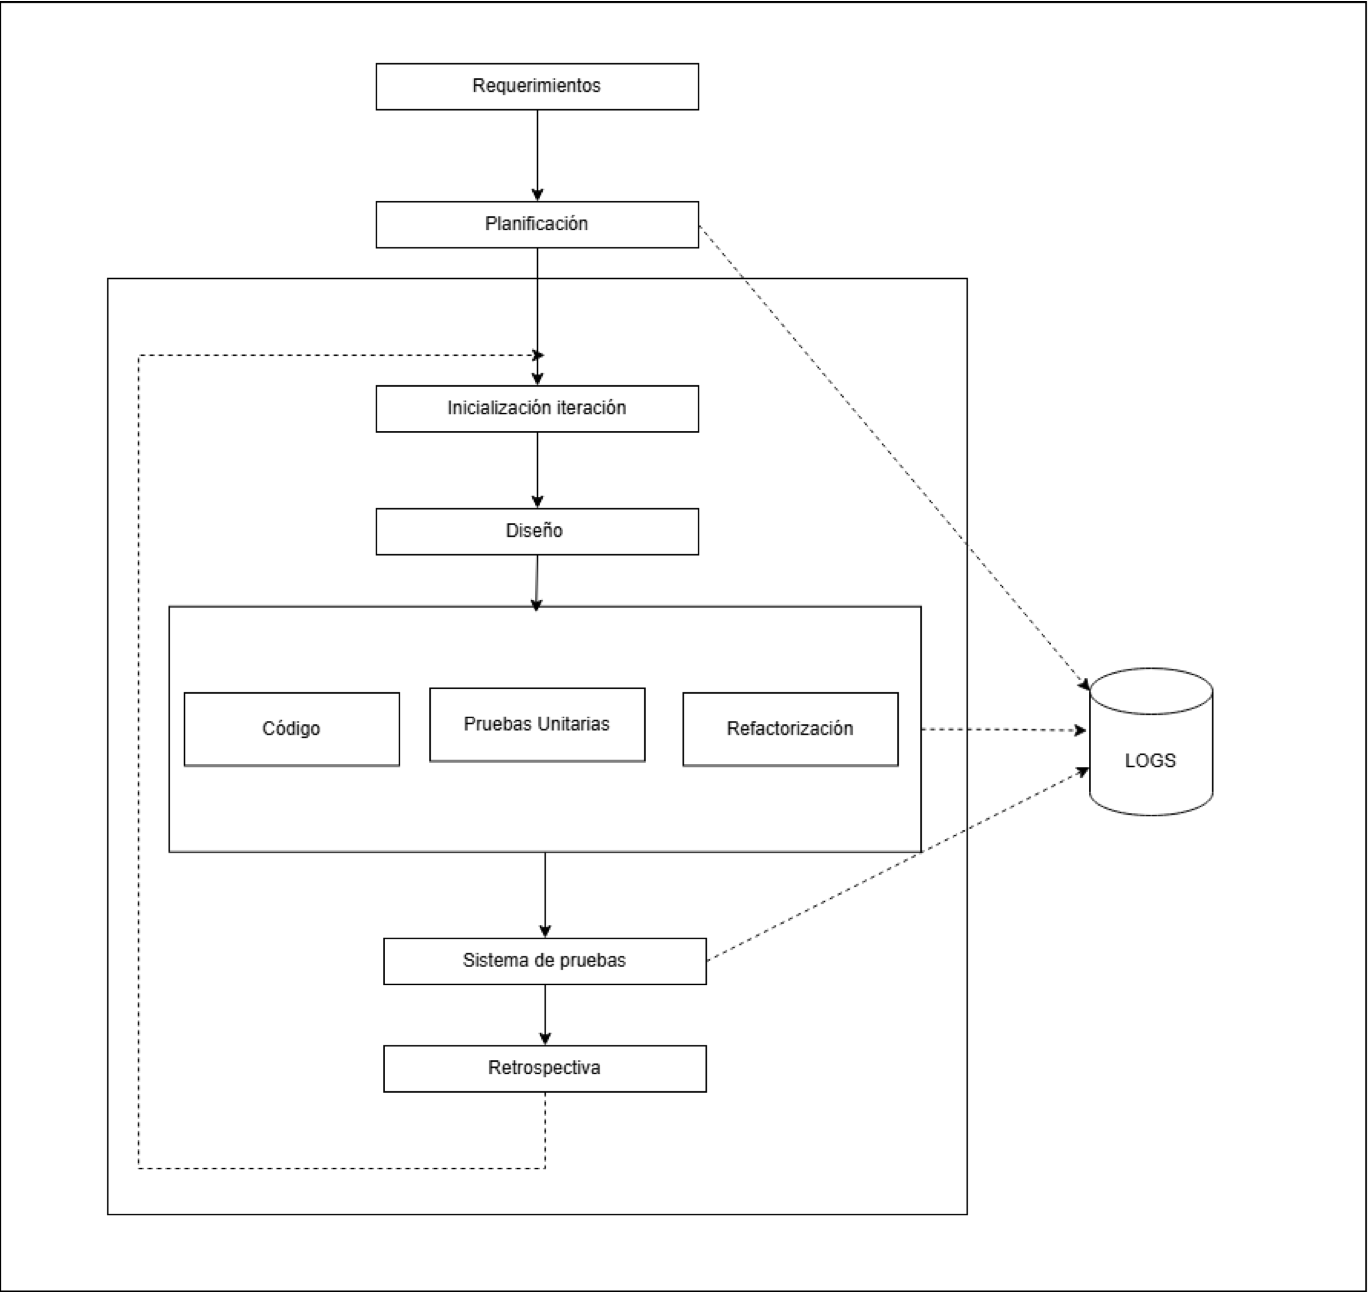
\includegraphics[width=0.8\textwidth]{fig-2-1-pxp}
  \caption[Fases de metodología Personal Extreme Programming (PXP)]{Fases de metodología Personal Extreme Programming (PXP).}
  \label{fig:pxp}
  \vspace{-2.9pt}
\end{figure}

\subsection{Metodologías de evaluación del proyecto }

En esta sección se describen las metodologías de evaluación que se implementarán para validar la calidad, usabilidad y efectividad del sistema desarrollado.

\subsubsection{Evaluación de Calidad}

Para asegurar que la plataforma esté libre de fallos críticos antes de su despliegue, se implementa una estrategia de pruebas a nivel de código y de sistema:

\begin{itemize}
  \item \textbf{Pruebas de Caja Blanca (Pruebas Unitarias y de Integración):} Estas pruebas se enfocan en verificar la lógica interna del código fuente, evaluando que los algoritmos críticos (como el motor de cálculo de cotizaciones y la lógica de proyección 3D) funcionen correctamente desde su interior. Se definen tests con el objetivo de alcanzar una cobertura de código de al menos un 95 \%.

  Para dar un ejemplo de las pruebas unitarias se considera realizar pruebas para funciones del código del programa, por ejemplo en el área de cotizaciones se ingresan valores a los insumos para verificar que los datos finales concuerden con los cálculos esperados en todo momento. A continuación, la Figura \ref{fig:cajablanca} ilustra el proceso de la prueba.

  \begin{figure}[H]
    \centering
    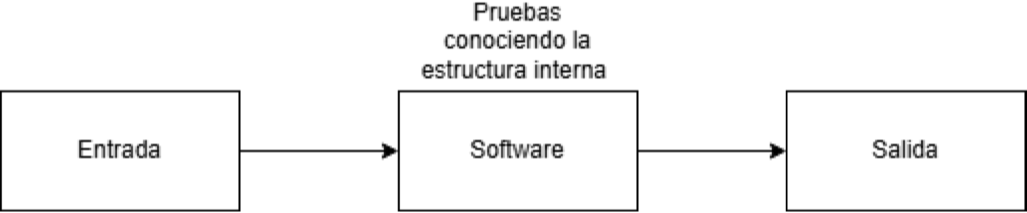
\includegraphics[width=0.6\textwidth]{fig-2-2-caja-blanca}
    \caption[Proceso de Prueba de Caja Blanca]{Proceso de Prueba de Caja Blanca.}
    \label{fig:cajablanca}
  \end{figure}

  \item \textbf{Pruebas de Caja Negra:} Corresponden a una forma de evaluar y validar el funcionamiento de los módulos del sistema sin necesidad de conocer su proceso interno. En estas pruebas, se definen entradas específicas (por ejemplo, subir un boceto y asignar horas) y se comparan con las salidas esperadas en la interfaz de usuario, garantizando que los módulos operen correctamente de extremo a extremo. A continuación, la Figura \ref{fig:cajanegra} ilustra el proceso de la prueba.

  \begin{figure}[H]
    \centering
    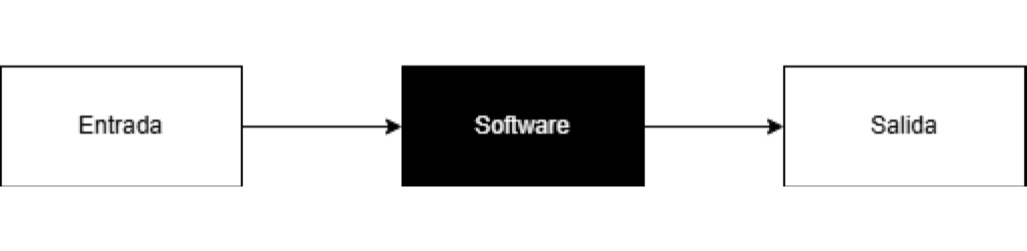
\includegraphics[width=0.6\textwidth]{fig-2-3-caja-negra}
    \caption[Proceso de Prueba de Caja Negra]{Proceso de Prueba de Caja Negra.}
    \label{fig:cajanegra}
    \vspace{9.42pt}
  \end{figure}
\end{itemize}

\subsubsection{Evaluación de Usabilidad y Aceptación}

Dado que el sistema está enfocado en usuarios finales (tatuadores y clientes del estudio), es fundamental validar que la interfaz sea intuitiva y el flujo de trabajo sea el adecuado.
\begin{itemize}
  \item \textbf{System Usability Scale (SUS)\cite{drew2018}:} Para evaluar la usabilidad empírica del sistema se considera aplicar el cuestionario estándar SUS. Este instrumento consiste en 10 afirmaciones evaluadas mediante una escala de Likert (desde ``Totalmente en desacuerdo'' hasta ``Totalmente de acuerdo''). A partir de las respuestas, se calcula un puntaje global. Para este proyecto, se ha establecido como métrica de éxito alcanzar un puntaje mínimo de 85 puntos, lo que clasificaría a la plataforma dentro de un rango de excelencia en términos de usabilidad.

  \item \textbf{Pruebas de Aceptación del Usuario (UAT)\cite{ponce}:} Se llevarán a cabo sesiones de prueba controladas donde el cliente experto y otros tatuadores invitados interactuan libremente con la versión final del sistema. Al finalizar, se registra su nivel de satisfacción, teniendo como meta alcanzar al menos un 90 \% de evaluación positiva respecto a la funcionalidad de la plataforma.
\end{itemize}

\subsubsection{Evaluación de Validación}

Para complementar las métricas de software y validar el impacto del sistema en el negocio, se considera un enfoque comparativo (Pre-test y Post-test) mediante entrevistas y análisis de registros:
\begin{itemize}
  \item \textbf{Entrevistas:} Se realiza entrevistas al inicio del proyecto para cuantificar las bases actuales del artista experto respecto a el tiempo que invierten en ajustar bocetos en papel, el tiempo que dedican a calcular costos manualmente, y su tasa de inasistencia semanal promedio.

  \item \textbf{Contraste de Resultados:} Una vez implementado el MVP y tras un periodo de prueba real, se vuelven a medir estos parámetros operando con el sistema. El objetivo es validar estadísticamente el logro en la reducción de los tiempos de previsualización en un 30 \% los tiempos de previsualización (módulo 3D), en un 40 \% los tiempos de cotización (módulo de inventario) y en un 50 \% el ausentismo (módulo de agendamiento con WhatsApp).
\end{itemize}

\section{Resumen capítulo}

En este capítulo se explicaron los conceptos básicos necesarios para entender el proyecto, se describieron las tecnologías a utilizar, evaluando alternativas y justificando la elección de cada una. También se revisó el estado del arte, presentando aplicaciones que ofrecen funcionalidades similares a la solución propuesta. Finalmente, detallaron las metodologías de desarrollo y evaluación, justificando la elección de cada una.

En el siguiente capítulo se abordará la aplicación de estas metodologías, junto con las adaptiones necesarias para el proyecto y los resultados esperados de los objetivos específicos.

% En el original la raya baja con la «g» de «Metodologías» (5 pt) sin mover el texto.
\titleformat{\chapter}[hang]
  {\normalfont\Huge\bfseries}{\thechapter.}{\dimexpr1.5em+2pt\relax}{}[\vspace{13.7pt}{\titlerule[2pt]}\vspace{-5pt}]
\chapter{Metodologías}

El presente capítulo está orientado a describir la manera en que se aplicará las metodologías propuestas en el capítulo anterior y los resultados esperados de los objeticos específicos.

\section{Personal Extreme Programming (PXP)}

Como se mencionó en el Capítulo 2.4.1, la metodología PXP adopta las mejores prácticas de las metodologías Personal Software Process (PSP) y Extreme Programming (XP). Se basa en un desarrollo personal pero a la vez sigue manteniendo las fases claves como Requerimientos, Planififcación e Iteración.

\subsection{Requerimientos }

Durante esta fase, se realiza una entrevista entre el desarrollador y el cliente para capturar los requerimientos iniciales del sistema. Estos requerimientos se transforman en la fase siguiente en historias de usuario, lo que permite enfocar el desarrollo en la experiencia del usuario.

\subsection{Planificación}

Durante esta fase, la actividad central consiste en la creación, priorización y organización de las historias de usuario (HU), las cuales se dividen y asignan a iteraciones específicas. En esta fase también se toman las decisiones de diseño de la aplicación, tales como las configuraciones base de las tecnologías a utilizar, arquitecturas de software y mockups, que permitirán el flujo de las distitnas vistas que tendrá la aplicación y su interacción con los usuarios.

\tituloparpegado{Historias de usuario}
A continuación, la Tabla \ref{tab:hu} ilustra las historias de usuario obtenidas a partir de la entrevista inicial con el cliente.

\begin{longtable}{|l|p{3.5cm}|p{9.5cm}|}
  \caption{Historias de Usuario} \label{tab:hu}\\
  \hline
  \textbf{HU} & \textbf{Actor(es)} & \textbf{Descripción} \\
  \hline
  \endfirsthead
  \multicolumn{3}{c}{\textbf{\tablename\ \thetable{} -- Continuación de la página anterior}} \\
  \hline
  \textbf{HU} & \textbf{Actor(es)} & \textbf{Descripción} \\
  \hline
  \endhead
  \hline
  \multicolumn{3}{|r|}{Continúa en la siguiente página...} \\
  \hline
  \endfoot
  \hline
  \endlastfoot
  HU01 & Tatuador & quiero registrarme en la plataforma ingresando mis datos, para tener un espacio de trabajo integral. \\ \hline
  HU02 & Tatuador & quiero iniciar y cerrar sesión mediante mis credenciales, para proteger la privacidad de mi negocio. \\ \hline
  HU03 & Tatuador & quiero recuperar mi contraseña en caso de olvido, para no perder el acceso a mi agenda e inventario. \\ \hline
  HU04 & Tatuador & quiero importar imágenes a la plataforma, para almacenarlas en la nube. \\ \hline
  HU05 & Tatuador & quiero ver todos mis diseños en una galería, para acceder a ellas de manera expedita. \\ \hline
  HU06 & Tatuador & quiero eliminar un boceto antiguo de la galería, para mantener mi espacio ordenado y liberar almacenamiento. \\ \hline
  HU07 & Tatuador & quiero añadir etiquetas a mis bocetos, para filtrarlos y encontrarlos ágilmente frente al cliente. \\ \hline
  HU08 & Tatuador & quiero elegir entre distintos modelos anatómicos 3D ya integrados, para utilizarlos como lienzo de previsualización. \\ \hline
  HU09 & Tatuador & quiero proyectar un boceto 2D (PNG) sobre el modelo 3D, para evaluar cómo se adapta a la curvatura de la piel. \\ \hline
  HU10 & Tatuador & quiero escalar, mover y rotar el diseño sobre el modelo 3D, para definir la posición exacta. \\ \hline
  HU11 & Tatuador & quiero registrar un material con su cantidad y costo unitario, para mantener un control inicial de mi stock. \\ \hline
  HU12 & Tatuador & quiero modificar el stock manual o borrar insumos descontinuados, para mantener la realidad operativa de mi estudio. \\ \hline
  HU13 & Tatuador & quiero visualizar una advertencia cuando un insumo llegue a un nivel crítico, para comprar reposiciones a tiempo. \\ \hline
  HU14 & Tatuador & quiero que el sistema calcule el costo de los insumos basándose en el tamaño del boceto y variables de trazado, para obtener un presupuesto automatizado. \\ \hline
  HU15 & Tatuador & quiero agregar o quitar materiales específicos sugeridos por el algoritmo, para refinar el cálculo final de la cotización. \\ \hline
  HU16 & Tatuador & quiero que al dar por finalizada una sesión cotizada los materiales se descuenten solos, para automatizar el control de stock. \\ \hline
  HU17 & Tatuador & quiero agendar a un cliente especificando fecha, hora, número de contacto y precio del proyecto, para organizar mis tiempos. \\ \hline
  HU18 & Tatuador & quiero ver mis citas en un formato de calendario mensual y semanal, para organizar visualmente mi jornada. \\ \hline
  HU19 & Tatuador & quiero poder crear distintos proyectos para clientes específicos junto con sus sesiones. \\ \hline
  HU20 & Tatuador & quiero poder subir una foto de cada sesión para ver los progresos del proyecto. \\ \hline
  HU21 & Tatuador & quiero cambiar la fecha de una cita o cancelarla, para mantener la agenda actualizada frente a imprevistos. \\ \hline
  HU22 & Tatuador & quiero que el sistema envíe automáticamente un mensaje de WhatsApp 24 horas antes de la sesión, para evitar olvidos o retrasos. \\ \hline
  HU23 & Tatuador & quiero que al cancelar o cambiar una hora el sistema avise al cliente por WhatsApp, para mantener una comunicación profesional. \\ \hline
  HU24 & Tatuador & quiero ver el historial de todas las sesiones pasadas y futuras asociadas a un cliente, para hacer seguimiento de piezas grandes. \\ \hline
  HU25 & Tatuador & quiero ver un panel de control al iniciar sesión con las citas programadas y alertas de stock bajo, para organizar mi jornada de un vistazo. \\ \hline
  HU26 & Tatuador & quiero visualizar una suma básica de los ingresos generados en el mes actual, para evaluar la rentabilidad del estudio. \\ \hline
  HU27 & Tatuador & quiero definir mis días y horas de trabajo, para que el calendario bloquee automáticamente mis días libres. \\ \hline
  HU28 & Tatuador & quiero poder editar el texto base del mensaje que se envía por WhatsApp, para darle recomendaciones del trato del tatuajes posteriormente al trabajo realizado. \\ \hline
  HU29 & Tatuador & quiero tener el resgistro de todos mis clientes atendidos con su información. \\ \hline
  HU30 & Tatuador & quiero poder visualizar un marcardor de todos mis clientes y asignarles puntaje para saber su responsabilidad de llegada y poder filtrarlos de acuerdo a ello. \\ \hline
  HU31 & Administrador & quiero registrar nuevos estudios de tatuaje en la plataforma indicando nombre, correo y plan contratado, para incorporar a nuevos clientes del sistema. \\ \hline
  HU32 & Administrador & quiero activar o desactivar una cuenta de estudio, para gestionar el acceso a la plataforma ante impagos o solicitudes de baja. \\ \hline
  HU33 & Administrador & quiero agregar tatuadores adicionales dentro de un estudio existente, para dar soporte a estudios con más de un profesional. \\ \hline
  HU34 & Administrador & quiero eliminar o desactivar la cuenta de un tatuador específico dentro de un estudio, para mantener actualizada la nómina de usuarios activos. \\ \hline
  HU35 & Administrador & quiero visualizar un listado de todos los estudios y tatuadores registrados, para monitorear el uso general de la plataforma. \\ \hline
  HU36 & Administrador & quiero ver métricas globales de uso por estudio (número de sesiones, citas agendadas, bocetos almacenados), para evaluar la adopción de la plataforma. \\ \hline
  HU37 & Administrador & quiero gestionar los modelos anatómicos 3D disponibles en la plataforma (agregar, actualizar o eliminar), para mantener actualizado el catálogo compartido entre estudios. \\ \hline
  HU38 & Administrador & quiero restablecer la contraseña de cualquier usuario registrado, para brindar soporte ante bloqueos de acceso. \\
\end{longtable}

\tituloparpegado{Priorización y estimación de historias de usuario}
En PXP, luego de realizar la creación de historias de usuario, se deben priorizar y estimar en base al esfuerzo que toma implementar cada una. Para priorizar se utiliza una escala que va desde el valor más bajo correspondiente a ``Baja'' hasta ``Crítica'' siendo el valor más alto, categorizándolas en base a su impacto sobre los objetivos específicos del proyecto.\\
\indent Por el lado de la estimación, si bien existen distintos métodos, se utilizará Planning Poker\cite{planningpoker}, el cual se elige debido a que emplea la escala de la serie de Fibonacci\cite{viggiani2006} para estimar cada historia, en el que entre más bajo sea el número otorgado, representará un menor esfuerzo técnico y cognitivo. A continuación, la Tabla \ref{tab:prioridad} ilustra el resultado de los métodos mencionados aplicados al catálogo del sistema.

\begin{longtable}{|c|c|c|}
  \caption{Priorización y estimación de esfuerzo para cada historia de usuario} \label{tab:prioridad}\\
  \hline
  \textbf{HU} & \textbf{Priorización} & \textbf{Estimación de esfuerzo} \\
  \hline
  \endfirsthead
  \multicolumn{3}{c}{\textbf{\tablename\ \thetable{} -- Continuación de la página anterior}} \\
  \hline
  \textbf{HU} & \textbf{Priorización} & \textbf{Estimación de esfuerzo} \\
  \hline
  \endhead
  \hline
  \multicolumn{3}{|r|}{Continúa en la siguiente página...} \\
  \hline
  \endfoot
  \hline
  \endlastfoot
  HU01 & Crítica & 3 \\ \hline
  HU02 & Crítica & 2 \\ \hline
  HU03 & Media & 3 \\ \hline
  HU04 & Crítica & 3 \\ \hline
  HU05 & Alta & 3 \\ \hline
  HU06 & Baja & 2 \\ \hline
  HU07 & Media & 3 \\ \hline
  HU08 & Crítica & 5 \\ \hline
  HU09 & Crítica & 8 \\ \hline
  HU10 & Crítica & 8 \\ \hline
  HU11 & Alta & 3 \\ \hline
  HU12 & Media & 2 \\ \hline
  HU13 & Baja & 2 \\ \hline
  HU14 & Crítica & 5 \\ \hline
  HU15 & Media & 3 \\ \hline
  HU16 & Alta & 5 \\ \hline
  HU17 & Crítica & 5 \\ \hline
  HU18 & Alta & 3 \\ \hline
  HU19 & Media & 3 \\ \hline
  HU20 & Alta & 3 \\ \hline
  HU21 & Alta & 5 \\ \hline
  HU22 & Crítica & 5 \\ \hline
  HU23 & Alta & 3 \\ \hline
  HU24 & Media & 3 \\ \hline
  HU25 & Media & 3 \\ \hline
  HU26 & Baja & 2 \\ \hline
  HU27 & Media & 2 \\ \hline
  HU28 & Baja & 2 \\ \hline
  HU29 & Media & 3 \\ \hline
  HU30 & Media & 3 \\ \hline
  HU31 & Crítica & 3 \\ \hline
  HU32 & Crítica & 2 \\ \hline
  HU33 & Alta & 3 \\ \hline
  HU34 & Media & 2 \\ \hline
  HU35 & Alta & 3 \\ \hline
  HU36 & Media & 5 \\ \hline
  HU37 & Media & 3 \\ \hline
  HU38 & Baja & 2 \\
\end{longtable}

\tituloparpegado{Planificación de historias de usuario}
A continuación, la Tabla \ref{tab:iteraciones} ilustra las iteraciones y las historias de usuario asociadas a cada una de ellas, distribuidas estratégicamente a lo largo de la fase de implementación del proyecto.
\begin{table}[h]
  \centering
  \caption{Asignación de historias de usuario a iteraciones}
  \label{tab:iteraciones}
  \renewcommand{\arraystretch}{1.2}
  \begin{tabular}{|c|c|}
    \hline
    \textbf{Iteración} & \textbf{Historias de usuario} \\
    \hline
    2 & HU01, HU02, HU03 \\ \hline
    3 & HU04, HU05, HU06, HU07 \\ \hline
    4 & HU11, HU12, HU13, HU25, HU26 \\ \hline
    5 & HU14, HU15, HU16, HU27 \\ \hline
    6 & HU17, HU18, HU19, HU20, HU24, HU30 \\ \hline
    7 & HU21, HU22, HU23, HU28, HU29, HU31 \\ \hline
    8 & HU08, HU09, HU10 \\ \hline
    9 & HU32, HU33, HU34, HU38 \\ \hline
    10 & HU35, HU36, HU37 \\ \hline
  \end{tabular}
\end{table}

\subsection{Iteración}

La fase de iteración es la de mayor duración en la metodología, y está dividida en varias etapas: Inicio de Iteración, Diseño, Implementación, Sistema de Pruebas y Retrospectiva. A continuación, se describe la implementación de cada una de estas etapas.

\titulopar{Inicio de iteración}

En esta etapa, se crean las tareas específicas para cada historia de usuario correspondiente a la iteración actual. Para llevar un control de la tareas y su estado de avance, se utiliza Trello. A continuación, la Figura \ref{fig:trello} muestra un ejemplo de cómo se organizan las tareas en el tablero de Trello, con columnas que representan los distintos estados del desarrollo (Por hacer, En progreso, En revisión, Completado) y tarjetas que detallan cada tarea específica asociada a las historias de usuario asignadas a la iteración.

\begin{figure}[H]
  \centering
  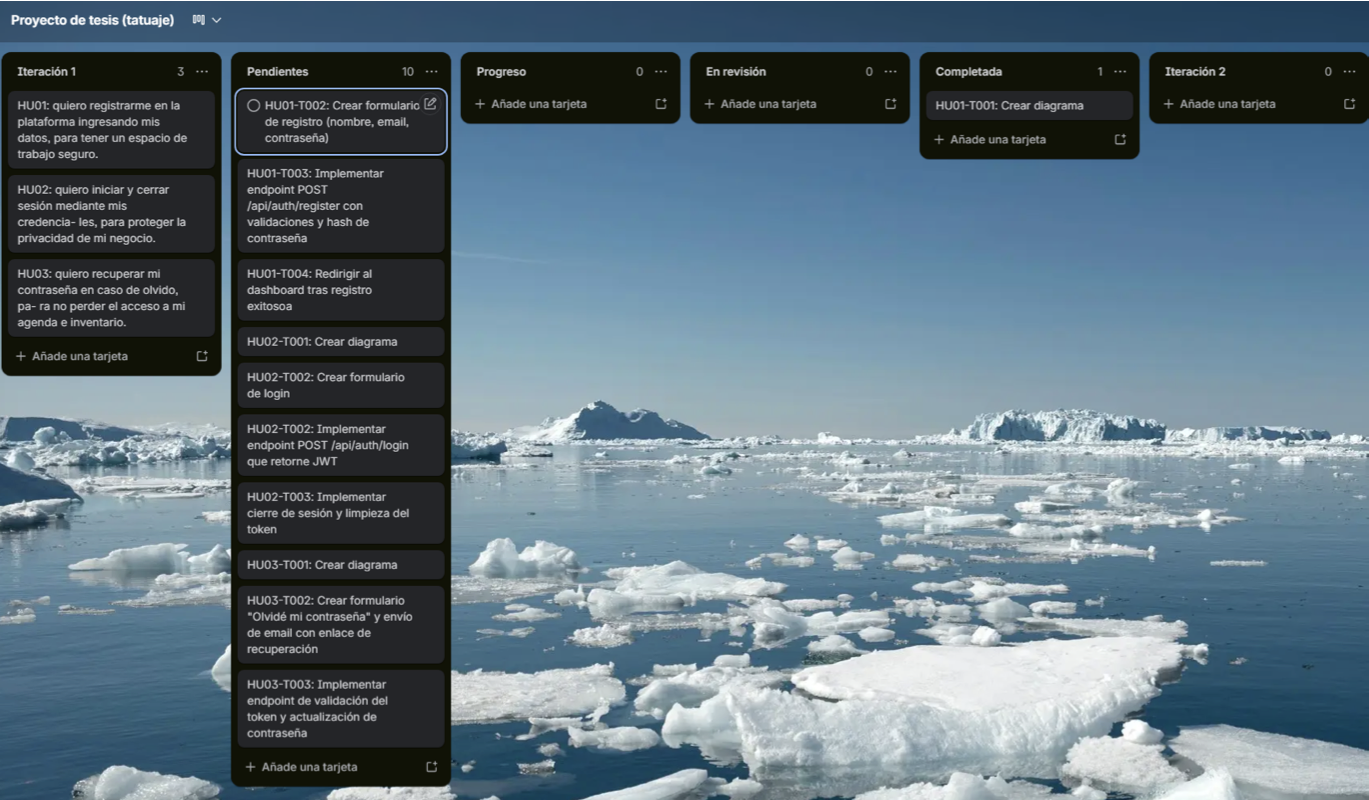
\includegraphics[width=0.8\textwidth]{fig-3-1-trello}
  \caption[Trello]{Extracto de la tabla dee registro de tareas por iteración.}
  \label{fig:trello}
\end{figure}

\titulopar{Diseño}

En esta etapa, se crean los diagramas de sencuencia de las historias de usuario asociadas a la iteración. A continuación, la Figura \ref{fig:secuencia} representa un ejemplo de diagrama de secuencia para el inicio de sesión.

\begin{figure}[H]
  \centering
  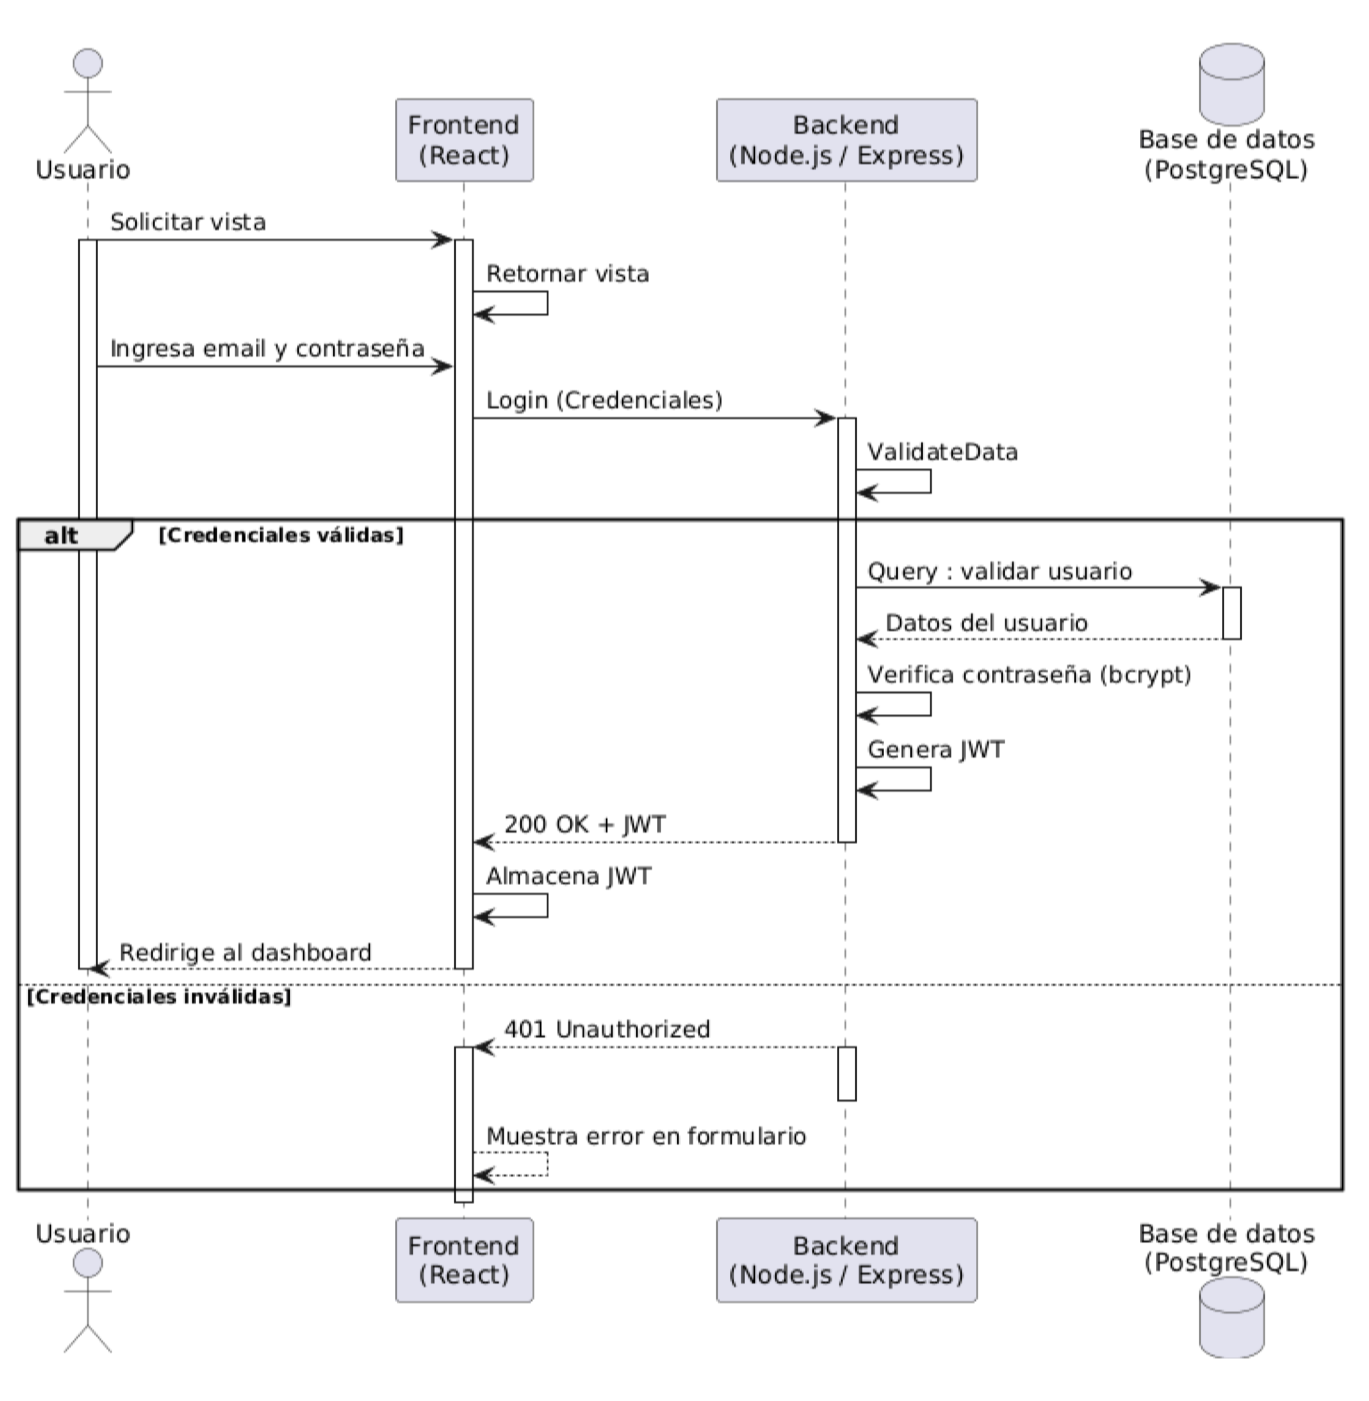
\includegraphics[width=0.8\textwidth]{fig-3-2-diagrama-secuencia}
  \caption[Diagrama de secuencia]{Ejemplo de diagrama de secuencia para el inicio de sesión.}
  \label{fig:secuencia}
\end{figure}

\titulopar{Implementación}

En esta etapa se lleva a cabo el desarrollo de código, pruebas unitarias y refactorización. La implementación sigue los diagramas de secuencia para guiar el flujo de las funcionalidades y los mockups propuestos. Aunque la metodología PXP sugiere un enfoque de Test-Driven Development (TDD)\cite{beck2002}, en el que primero se crean las pruebas, luego el código, y finalmente se realiza la refactorización este caso se ajustaría el proceso: primero se desarrollará el código, luego se completarán las pruebas unitarias, y se refactorizará en caso de que alguna prueba falle.

\titulopar{Sistema de pruebas}

En esta etapa se crean y ejecutan las pruebas correspondientes a todas las tareas definidas en el Inicio de Iteración. Si alguna de las pruebas falla, se regresa a la etapa de Implementación para realizar la refactorización necesaria y asegurar que el código cumpla con los requisitos definidos en las historias de usuario. Para llevar el control de las pruebas se utiliza una lista de verifiación en el mismo Trello a cada tarea, en donde se marcan las pruebas que han sido superadas y las que aún están pendientes o han fallado.

A continuación la Figura \ref{fig:checklist} muestra un ejemplo de una lista de verificación para una iteración en particular.

\begin{figure}[H]
  \centering
  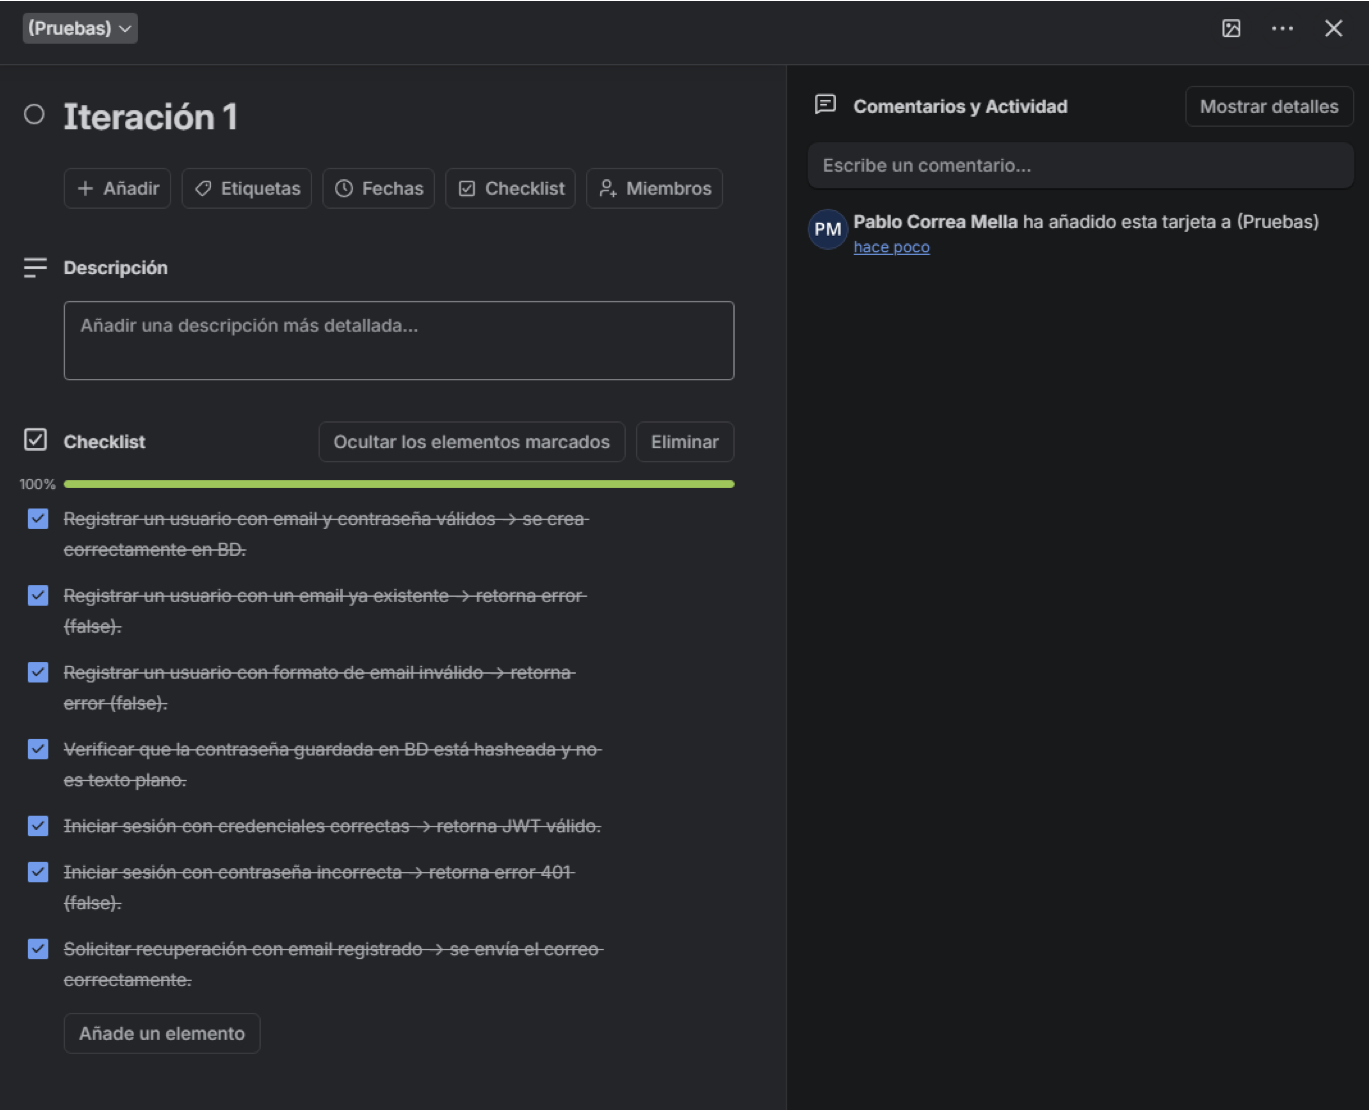
\includegraphics[width=0.8\textwidth]{fig-3-3-lista-verificacion}
  \caption[Lista de verificación de pruebas]{Ejemplo de lista de verificación de pruebas para una iteración.}
  \label{fig:checklist}
\end{figure}

\titulopar{Retrospectiva}

En esta etapa se realiza un análisis del desempeño del desarrollo, se integran las recomendaciones o ajustes detectados por el usuario experto, y se planifica el inicio de la siguiente iteración o el cierre definitivo del proyecto. Para llevar un control de las recomendaciones y ajustes, se utiliza una sección específica en Trello donde se documentan los comentarios recibidos durante la fase de pruebas, así como las acciones a tomar para mejorar el sistema en la siguiente iteración.

\section{Evaluación}

Como se mencionó en el Capítulo 2.5.2 para eevaluar el cumplimiento el objetivo general y los objetivos específicos, se implementarán distintas metodologías de evaluación, las cuales se describen a continuación.

\subsection{Prueba de caja negra}

Las pruebas de caja negra se enfocan en evaluar el funcionamiento de los módulos del sistema sin necesidad de conocer su proceso interno. En estas pruebas, se definen entradas específicas (por ejemplo, subir un boceto y asignar horas) y se comparan con las salidas esperadas en la interfaz de usuario, garantizando que los módulos operen correctamente de extremo a extremo. Para llevar un control de las pruebas de caja negra, se registran en una hoja de cálculo donde se documentan los casos de prueba definidos, las entradas utilizadas, las salidas esperadas y los resultados obtenidos, permitiendo así un seguimiento detallado del proceso de validación. A continuación, la Figura \ref{fig:registrocajanegra} muestra un ejemplo de cómo se registra una prueba de caja negra en la hoja de cálculo.

\begin{figure}[H]
  \centering
  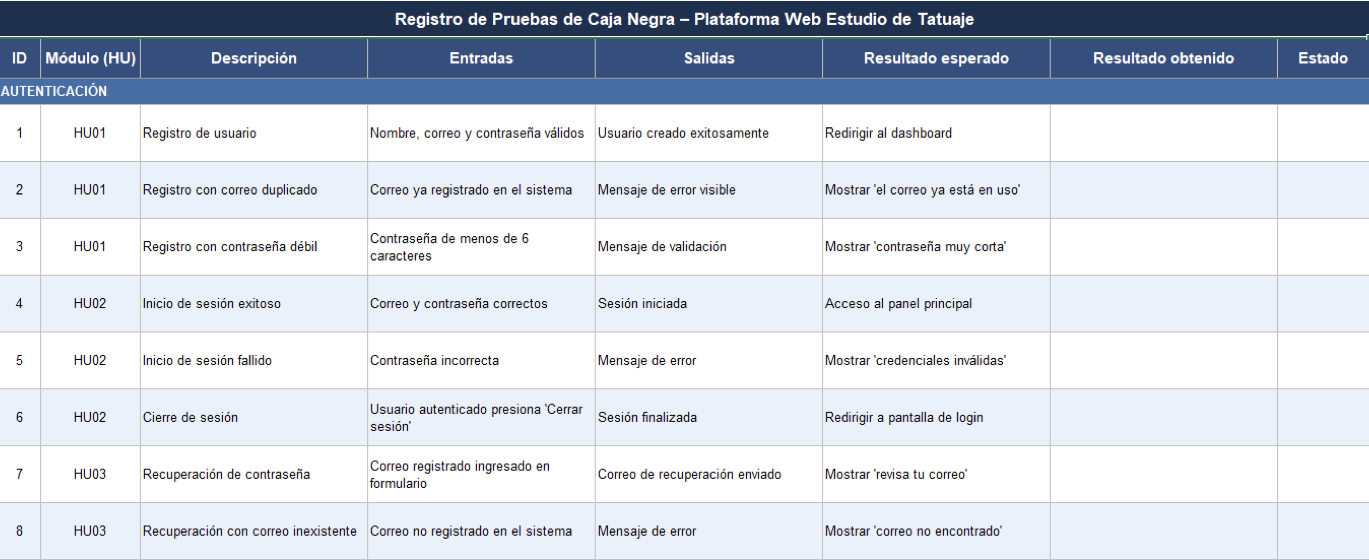
\includegraphics[width=0.8\textwidth]{fig-3-4-registro-caja-negra}
  \caption[Registro de prueba de caja negra]{Ejemplo de registro de prueba de caja negra en una hoja de cálculo.}
  \label{fig:registrocajanegra}
\end{figure}

\vspace{\parskip}
\subsection{Prueba de caja blanca }

Las pruebas de caja blanca se enfocan en verificar la lógica interna del código fuente, evaluando que los algoritmos críticos (como el motor de cálculo de cotizaciones y la lógica de proyección 3D) funcionen correctamente desde su interior. Se definen tests con el objetivo de alcanzar una cobertura de código de al menos un 95 \%. Para llevar un control de las pruebas de caja blanca, se utilizan herramientas de análisis de cobertura que generan reportes detallados sobre qué partes del código han sido ejecutadas durante las pruebas, permitiendo identificar áreas no cubiertas y asegurar que se cumpla con el objetivo establecido.

\subsection{Prueba de usabilidad}

La prueba de usabilidad SUS permite que el usuario final evalúe la aplicación mediante un cuestionario de 10 preguntas, que serán respondidas en una escala de Likert, con el objetivo de obtener una puntuación global que refleje la usabilidad del sistema. Para este proyecto, se ha establecido como métrica de éxito alcanzar un puntaje mínimo de 85 puntos, lo que indicaría que la plataforma es altamente usable y cumple con las expectativas del cliente experto. A continuación, se detallan las preguntas:

\vspace{\parskip}
\begin{enumerate}
  \item Creo que me gustaría usar esta plataforma con frecuencia.\\
  \item Encontré la plataforma innecesariamente compleja.\\
  \item Creo que la plataforma es fácil de usar.\\
  \item Creo que necesitaría la ayuda de una persona con conocimientos técnicos para usar esta plataforma.\\
  \item Creo que las funciones de esta plataforma están bien integradas.\\
  \item Creo que hay demasiada inconsistencia en esta plataforma.\\
  \item Imagino que la mayoría de las personas aprenderían a usar esta plataforma muy rápidamente.\\
  \item Creo que esta plataforma es muy difícil de usar.\\
  \item Creo que me sentiría muy seguro usando esta plataforma.\\
  \item Necesitaría aprender muchas cosas antes de poder usar esta plataforma.\\
\end{enumerate}
\vspace{\parskip}

Para obtener el grado de aceptación de la aplicación se debe realizar el siguiente cálculo:

\begin{itemize}
  \item Sumar las puntuaciones de las preguntas impares (1, 3, 5, 7, 9) y restar 5 al resultado.
  \item Sumar las puntuaciones de las preguntas pares (2, 4, 6, 8, 10) y restar el resultado a 25.
  \item Sumar los resultados de ambos cálculos y multiplicar por 2.5 para obtener la puntuación final en una escala de 0 a 100.
\end{itemize}
\vspace{\parskip}

El puntaje final, que varía entre 0 y 100, permite clasificar la usabilidad de la plataforma como Inaceptable (0-49), Mediocre (50-68) o Aceptable (69-100).

\subsection{Encuesta}

Este método de evaluación, como se detalla en el Capítulo 2.5.2, permite medir objetivos específicos comparando el estado inicial y final de las métricas evaluadas. Las preguntas de la encuesta están diseñadas para obtener respuestas númericas, lo que facilita la comparación de ambos estasdos. A continuación, se presentan algunas de las preguntas, en este caso las que se utilizan para determinar el estado inicial de los objetivos específicos.

\vspace{\parskip}
\begin{enumerate}
  \item ¿Cuánto tiempo promedio dedicas a ajustar o posicionar un boceto en papel para que se adapte a la curvatura de la piel? (en minutos)\\
  \item ¿Cuánto tiempo promedio dedicas a calcular el costo de un tatuaje manualmente? (en minutos)\\
  \item ¿Cuál es tu tasa de inasistencia semanal promedio? (en porcentaje)\\
  \item ¿Cuánto tiempo promedio dedicas a gestionar tu agenda y enviar recordatorios a tus clientes? (en minutos)\\
  \item ¿Cuánto tiempo promedio dedicas a organizar tu inventario y calcular el costo de los insumos? (en minutos)\\
  \mbox{}\\[-1.01pt]
\end{enumerate}

\section{Resultados esperados}

A continuación, se detallan los resultados esperados para cada uno de los objetivos específicos planteados en el Capítulo 1.2.2:

\begin{itemize}
  \item \textbf{Reducción del ausentismo (Objetivo Específico 2):}
  \begin{itemize}
    \item Resultado esperado: Se espera lograr una reducción del 50 \% en la tasa de inasistencia semanal al implementar el módulo de agendamiento con recordatorios automáticos por WhatsApp, en comparación con la tasa actual sin este sistema.
    \item Pruebas para lograr resultado esperado: Prueba de que el funcionamiento del módulo de agendamiento y recordatorios automáticos por WhatsApp realice el envío correcto de los mensajes 24 horas antes de la sesión programada, y que el cliente reciba estos mensajes sin fallos.
  \end{itemize}
  \item \textbf{Reducción del tiempo de cotización (Objetivo Específico 3):}
  \begin{itemize}
    \item Resultado esperado: Se espera lograr una reducción del 40 \% en los tiempos de cotización al utilizar el módulo de inventario y cálculo automatizado, en comparación con el método manual de cálculo.
    \item Pruebas para lograr resultado esperado: Prueba de que el funcionamiento del módulo de inventario y cálculo automatizado permita calcular los costos de manera precisa y rápida, en comparación con el método manual.
  \end{itemize}
  \item \textbf{Reducción del tiempo de previsualización (Objetivo Específico 4):}
  \begin{itemize}
    \item Resultado esperado:Se espera lograr una reducción del 30 \% en los tiempos de previsualización al utilizar el módulo de proyección 3D, en comparación con el método tradicional de ajuste manual en papel.
    \item Pruebas para lograr resultado esperado: Prueba de que el funcionamiento del módulo de proyección 3D permita ajustar y posicionar los bocetos de manera rápida y precisa sobre el modelo anatómico, en comparación con el método manual en papel.
  \end{itemize}
\end{itemize}

\section{Resumen capítulo}

En este capítulo se presentó detallademente la forma en que se aplicará la metodología PXP en el proyecto. También, se explican las metodologías de evaluación, mediante pruebas de software y, pruebas cualititativas y cuantitativas, en donde se agregan ejemplos de estas. Finalmente, se mencionan los resultados esperados, los cuales responden a los objetivos específicos planteados en el Capítulo 1.2.2.

En el siguiente capítulo se detallará la implementación de la metodología de desarrollo, en donde se explicará el trabajo realizado en las iteraciones, siguiendo las etapas de inicio de iteración, diseño, implementación, sistema de pruebas y retrospectiva.

\titleformat{\chapter}[hang]
  {\normalfont\Huge\bfseries}{\thechapter.}{\dimexpr1.5em+2pt\relax}{}[\vspace{8.7pt}{\titlerule[2pt]}]
\chapter{Desarrollo}

El presente capítulo está orientado a presentar la implementación de la metodología de desarrollo.

\section{Diseño de software }

A continuación, se presentan elementos claves en el diseño de software, tales como arquitecturas, modelos de datos y mockups.

\subsection{Arquitectura física }

La arquitectura física implementada corresponde a un modelo cliente-servidor. Durante la fase de desarrollo y pruebas, todos los componentes del sistema se alojan en un entorno local, utilizando contenedores Docker, lo que garantiza la portabilidad del entorno y elimina dependencias de configuración entre máquinas.

Como se ilustra en la Figura \ref{fig:arqfisica}, el flujo de comunicación comienza cuando el dispositivo cliente realiza una petición a través de Internet hacia el servidor de Frontend, donde se sirve la aplicación React. Las interacciones dinámicas del usuario generan peticiones HTTP/HTTPS hacia el servidor Backend desarrollado en Node.js, el cual se comunica con dos servicios externos: el Servidor de Base de Datos PostgreSQL, encargado de la persistencia de datos, y la API de Mensajería de WhatsApp, responsable del envío de recordatorios automáticos a los clientes.

Esta separación en contenedores independientes facilita una eventual migración hacia servicios en la nube especializados.

\begin{figure}[H]
  \centering
  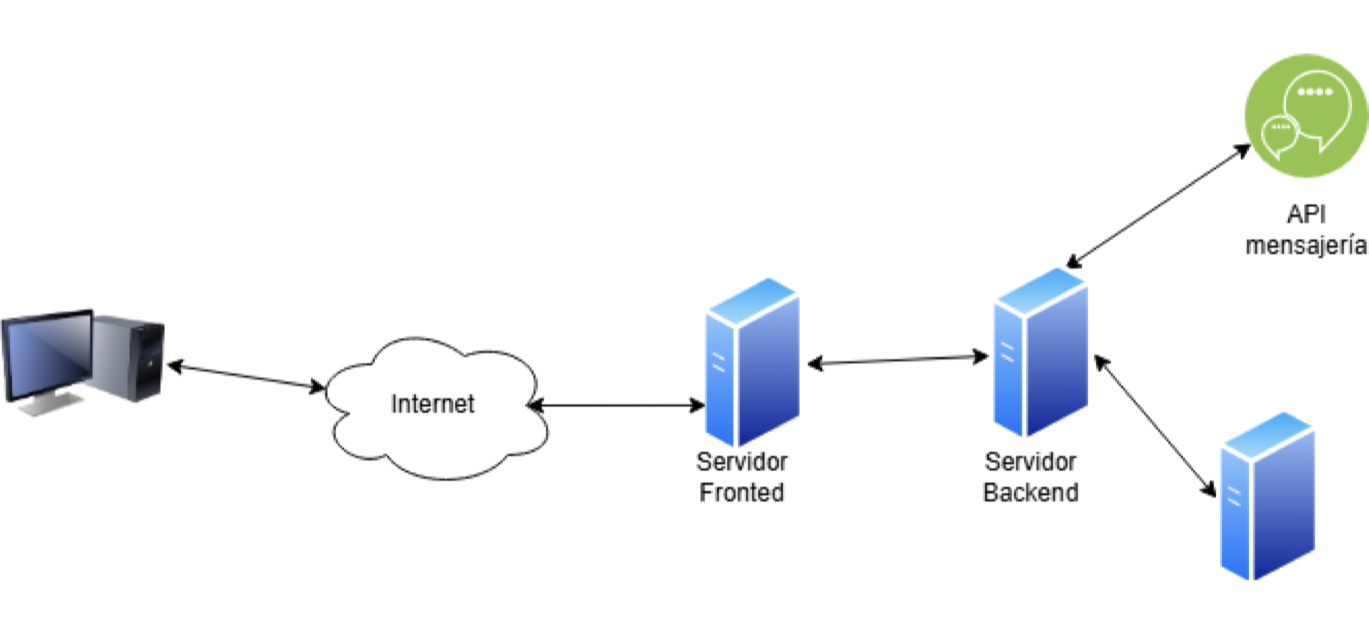
\includegraphics[width=0.8\textwidth]{fig-4-1-arquitectura-fisica}
  \caption[Arquitectura Física]{Arquitectura Física del Sistema.}
  \label{fig:arqfisica}
\vspace{-5.72pt}
\end{figure}

\subsection{Arquitectura lógica}

La arquitectura lógica propuesta sigue el patrón de tres capas.

\begin{figure}[h]
  \centering
  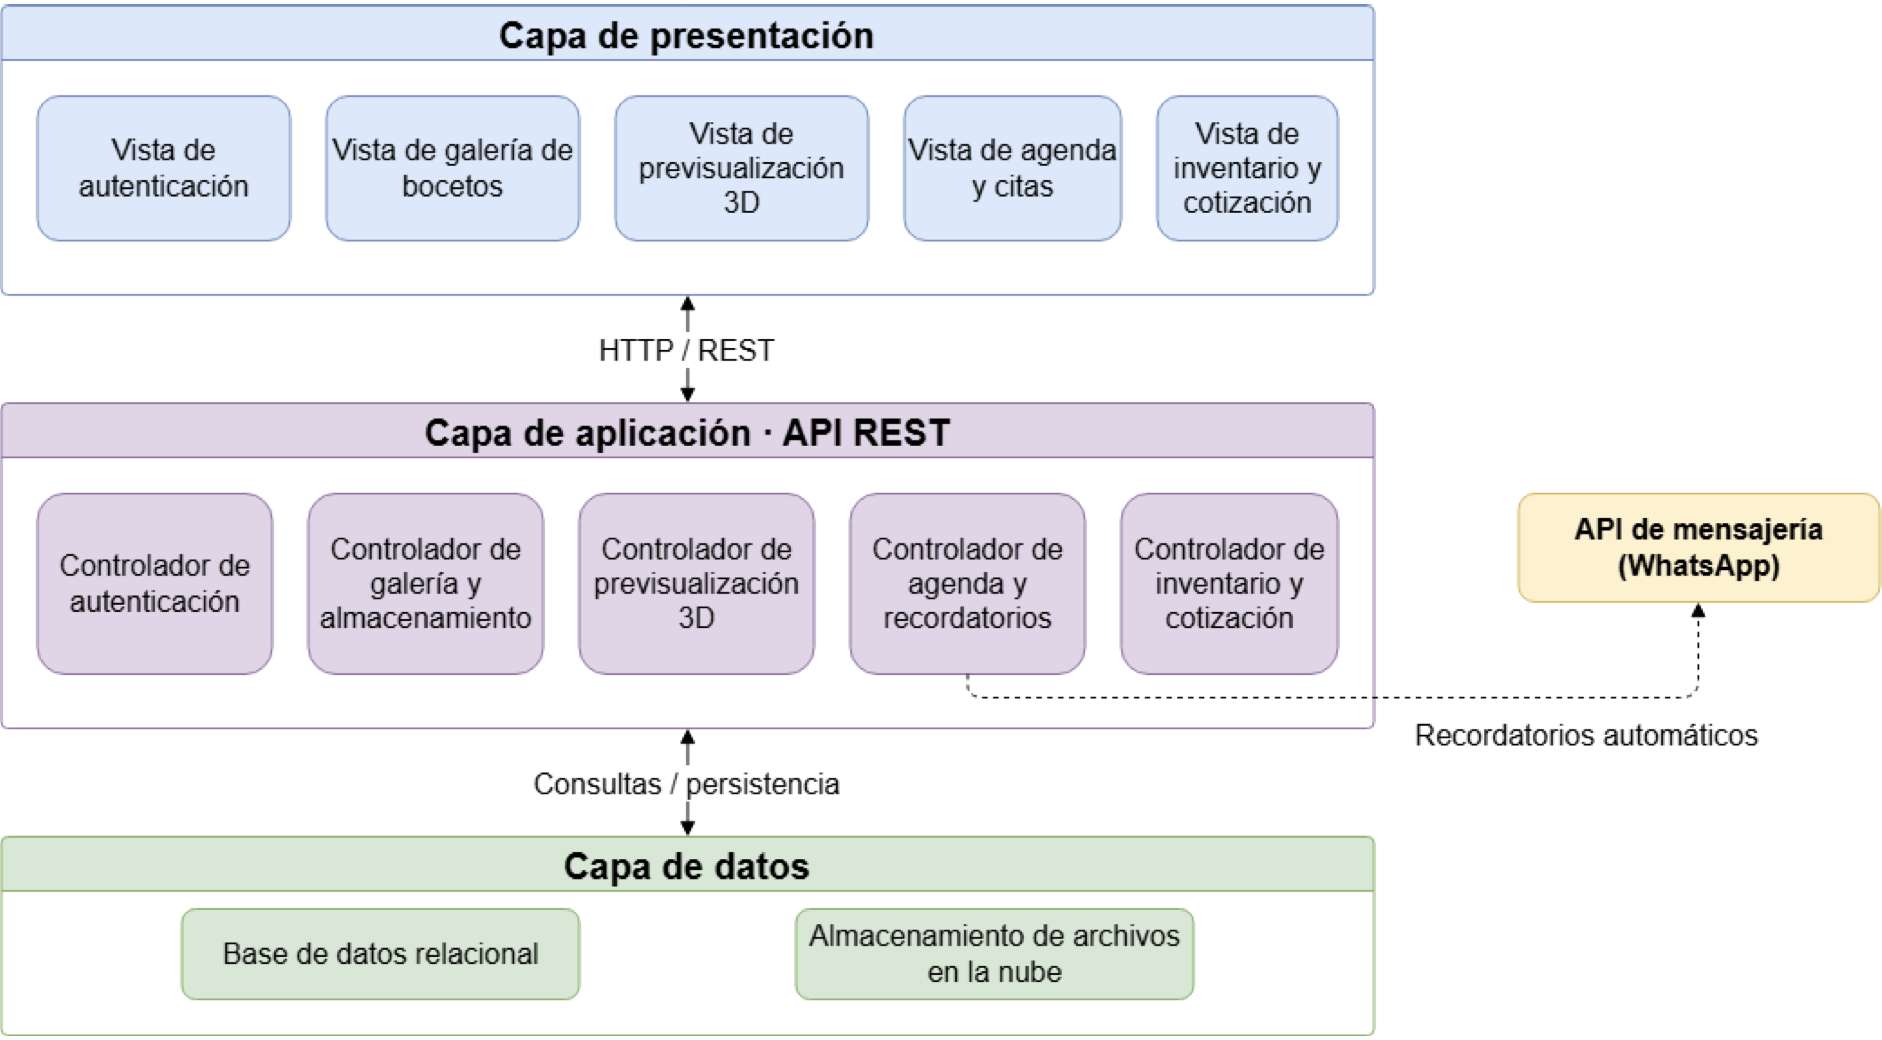
\includegraphics[width=1.1\textwidth]{fig-4-2-arquitectura-logica}
  \caption[Arquitectura Lógica]{Arquitectura Lógica del Sistema.}
  \label{fig:arqlogica}
\vspace{2.28pt}
\end{figure}

En la Figura \ref{fig:arqlogica} se ilustra la arquitectura lógica propuesta sigue el patrón de tres capas, ampliamente utilizado en el desarrollo de aplicaciones web modernas. Este patrón organiza el sistema en niveles de responsabilidad bien definidos, donde cada capa solo se comunica con la capa inmediatamente adyacente, lo que favorece la separación de responsabilidades, la mantenibilidad del código y la escalabilidad del sistema.

La capa de presentación corresponde a la interfaz de usuario ejecutada en el navegador del cliente. Esta capa es responsable de renderizar las vistas y gestionar la interacción del usuario, organizándose en módulos que corresponden a las funcionalidades principales del sistema: autenticación, galería de bocetos, previsualización 3D, agenda de citas, e inventario y cotización.

La capa de aplicación centraliza la lógica de negocio del sistema, expuesta mediante una API REST que recibe las solicitudes HTTP provenientes de la capa de presentación. Esta capa contiene los controladores de cada módulo, encargados de validar los datos de entrada, ejecutar las reglas de negocio como el algoritmo de cotización automática o el envío de recordatorios y coordinar las operaciones sobre la capa de datos.

La capa de datos es responsable de la persistencia del sistema. Se divide en dos componentes: la base de datos relacional, que almacena de forma estructurada los registros de usuarios, citas, inventario y cotizaciones, y el almacenamiento de archivos en la nube, dedicado a los bocetos en formato de imagen y los modelos anatómicos tridimensionales.

Adicionalmente, la capa de aplicación se integra con un servicio externo de mensajería para el envío automatizado de recordatorios a los clientes, manteniéndose esta integración desacoplada del resto del sistema mediante su propio controlador.

\subsection{Modelo de datos }

Como se mencionó en el Capítulo 2.3.3, el modelo de datos se basa en una base de datos relacional, utilizando PostgreSQL. A continuación, la Figura \ref{fig:er} muestra el diagrama entidad-relación del modelo de datos propuesto para el sistema.

\begin{figure}[H]
  \centering
  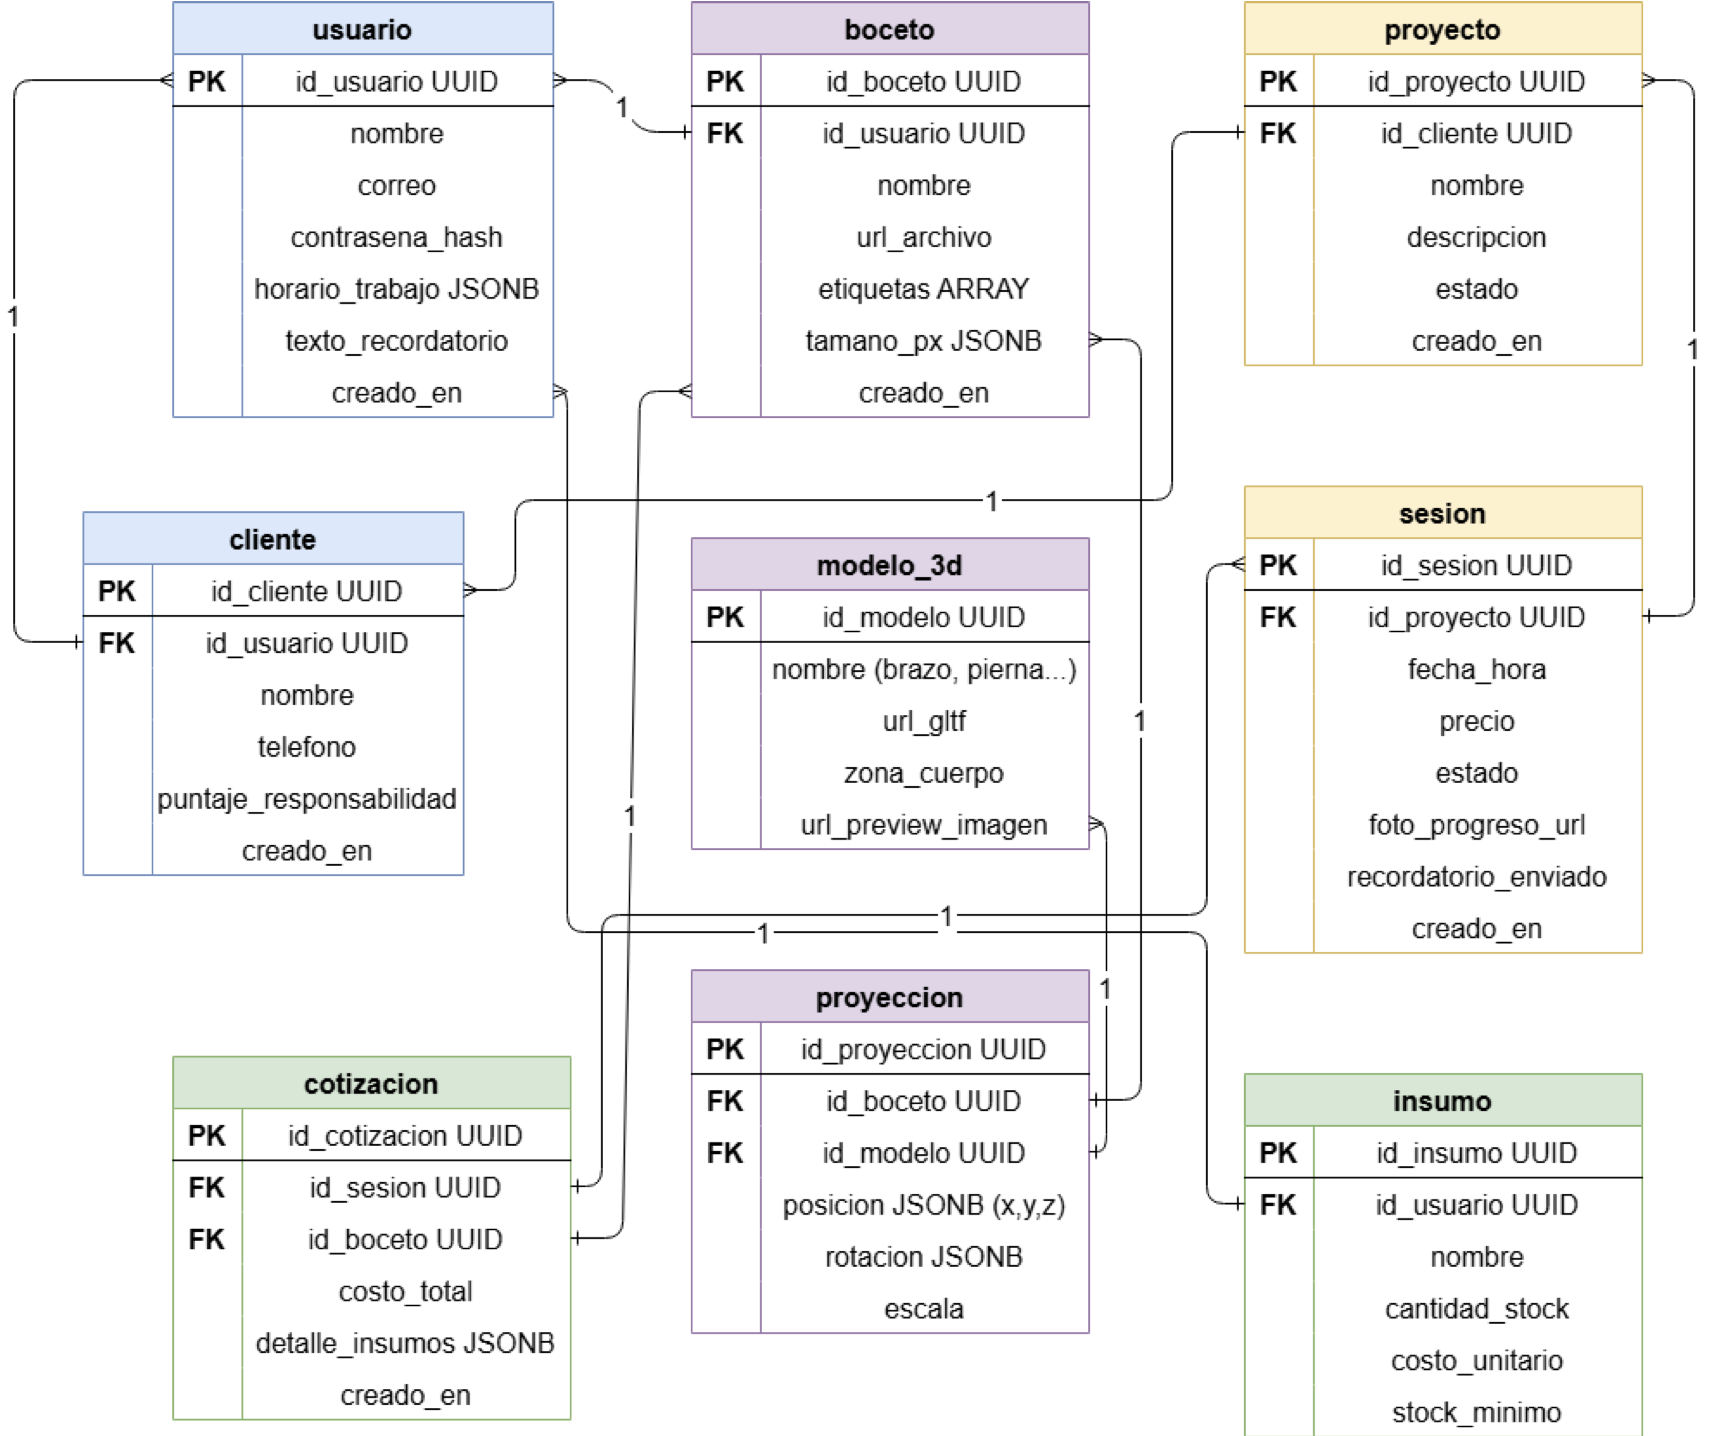
\includegraphics[width=\textwidth]{fig-4-3-diagrama-er}
  \caption[Diagrama Entidad-Relación]{Diagrama Entidad-Relación del modelo de datos del sistema.}
  \label{fig:er}
\end{figure}

\vspace{\parskip}
\subsection{Mockups}

En esta sección se presentan algunos de los mockups propuestos durante el proceso de desarrollo del sitema, los cuales fueron diseñados en base a los requerimientos funcionales y validos por la contrapartee. Estos mockups tienen como objetivo guiar el desarrollo de las principales interfaces del sistema y asegurando que cumplan con las expectativas del cliente experto.

\begin{figure}[H]
  \centering
  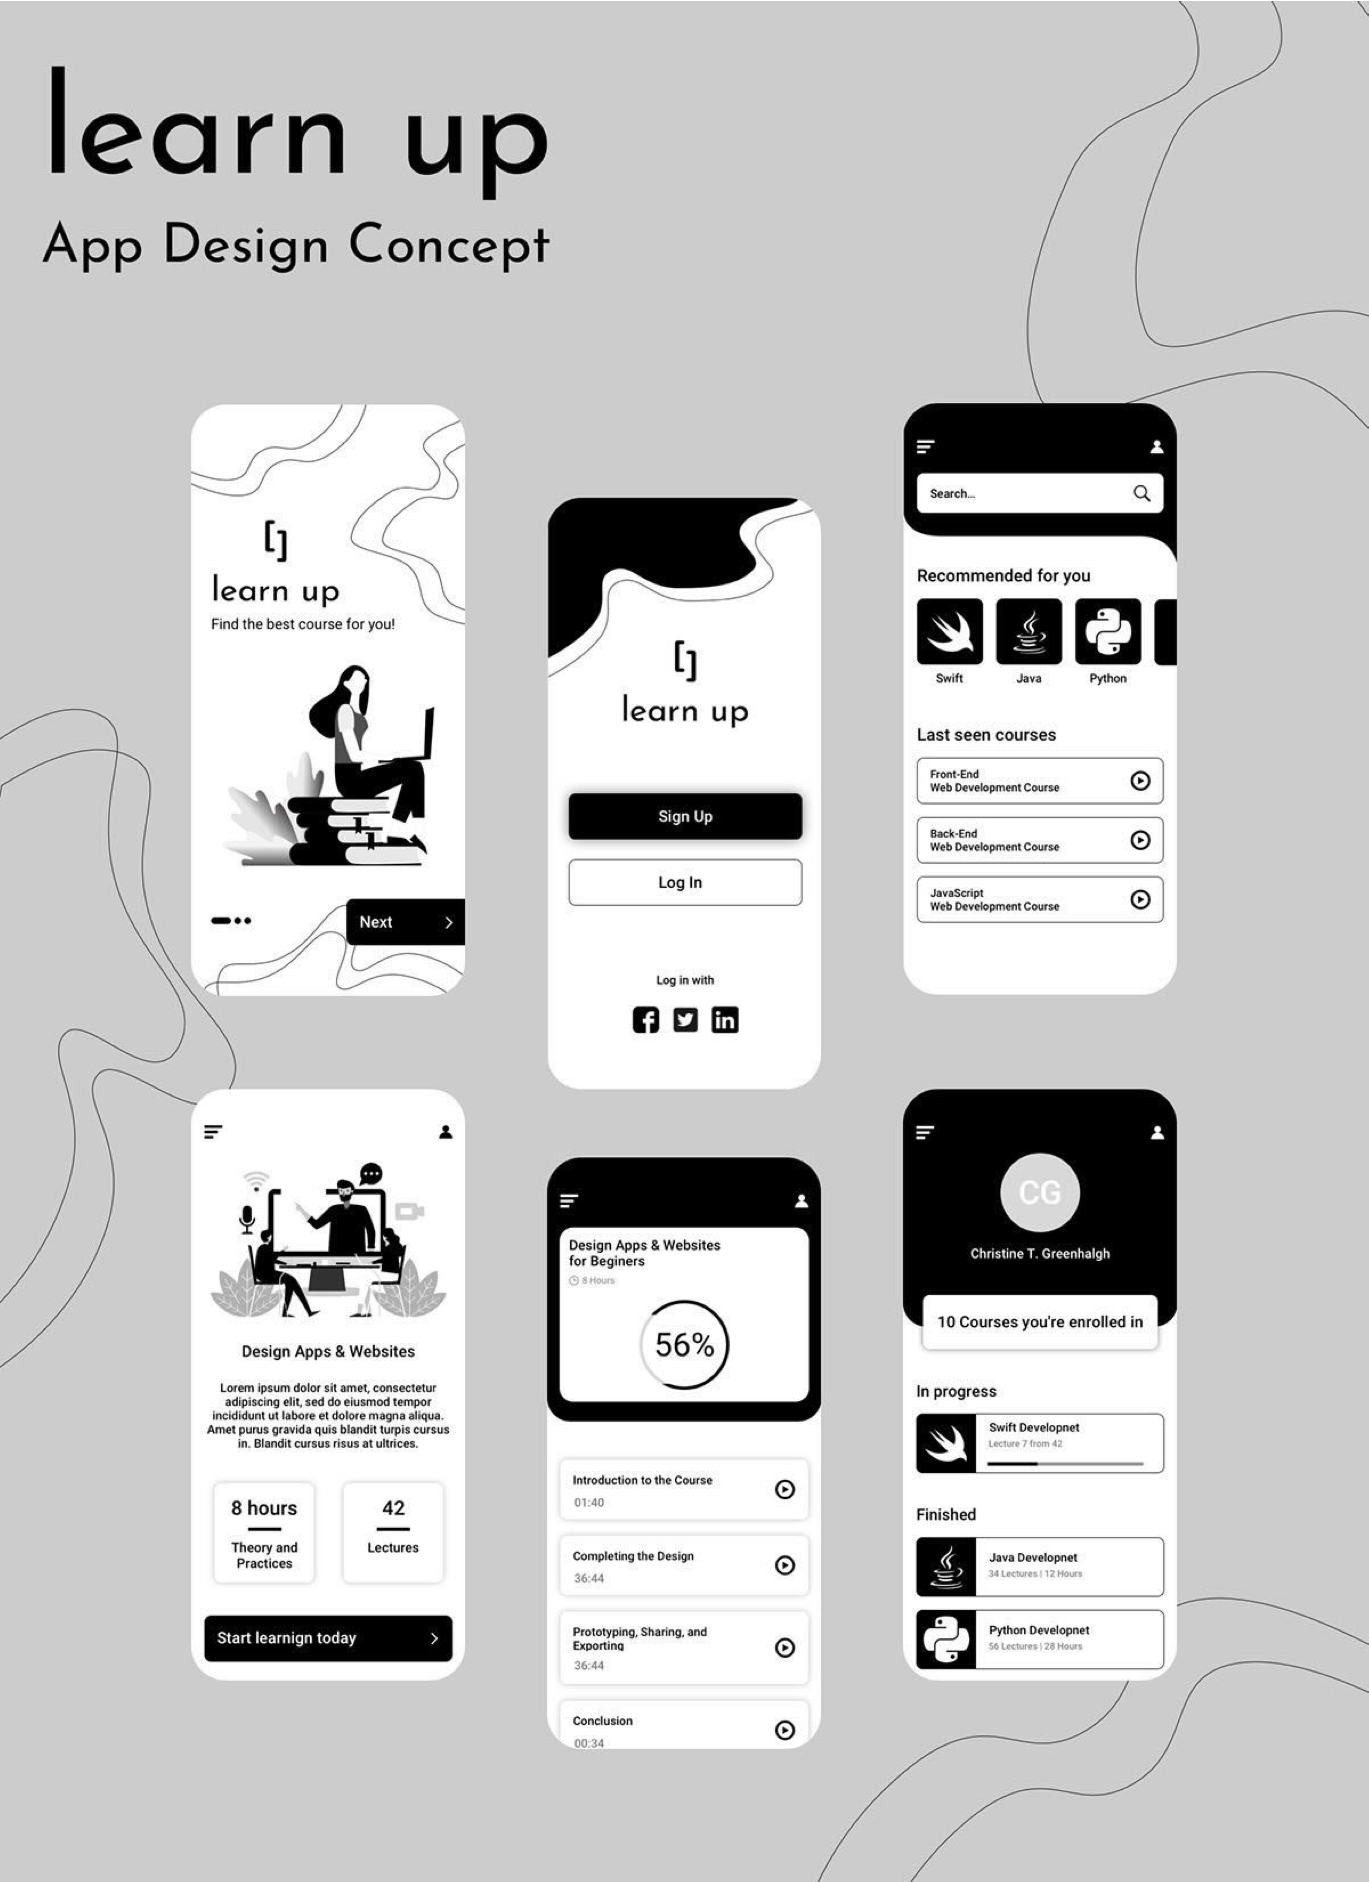
\includegraphics[width=0.8\textwidth]{fig-4-4-idea-1}
  \caption{Idea 1}
  \label{fig:idea1}
\end{figure}

\begin{figure}[H]
  \centering
  
\includegraphics[width=0.8\textwidth]{fig-4-5-idea-2}
  \caption{Idea 2}
  \label{fig:idea2}
\end{figure}

\begin{figure}[H]
  \centering
  
\includegraphics[width=0.8\textwidth]{fig-4-6-idea-3}
  \caption{Idea 3}
  \label{fig:idea3}
\end{figure}

En las Figuras \ref{fig:idea1}, \ref{fig:idea2} y \ref{fig:idea3} se presentan tres ideas de diseño para la interfaz de usuario del sistema, estas ideas fueron diseñadas por el usuario experto y buscan ser una guía visual para la elaboración de los mockups finales y la estética que se busca conseguir en la aplicación.

\begin{figure}[H]
  \centering
  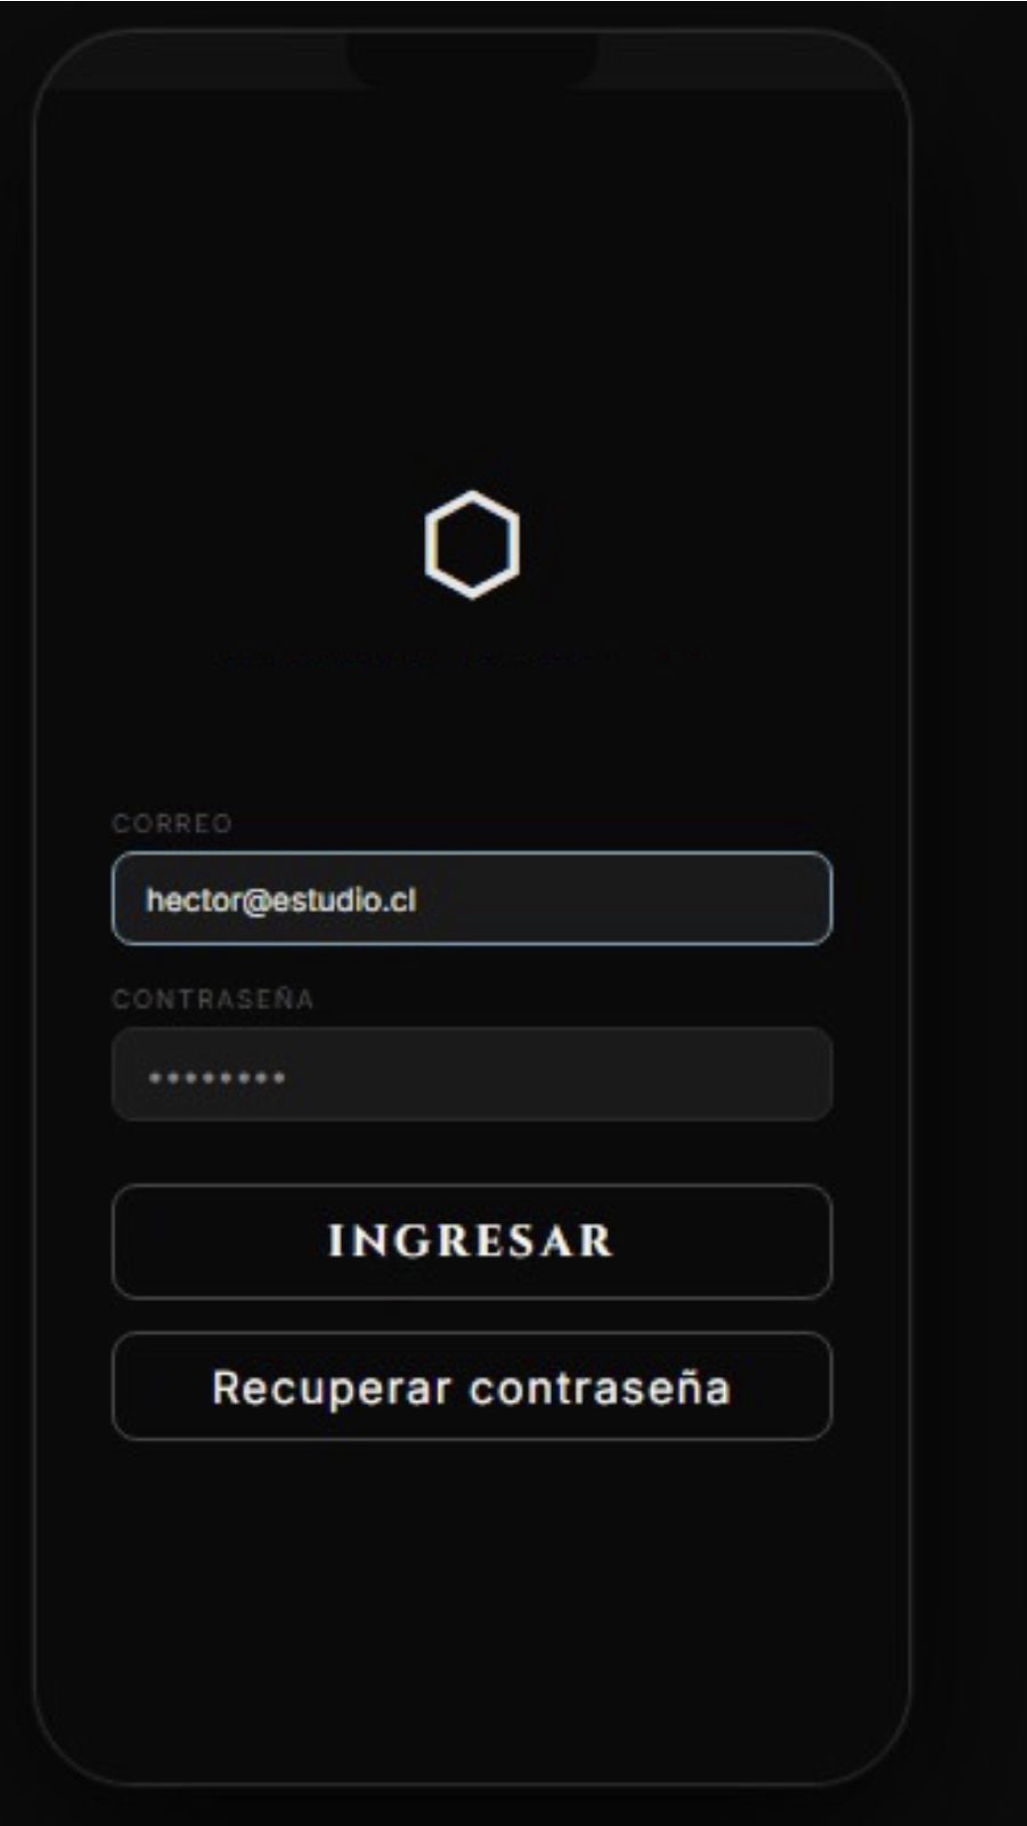
\includegraphics[width=0.6\textwidth]{fig-4-7-mockup-inicio-sesion}
  \caption[Mockup Inicio Sesión]{Mockup Inicio Sesión.}
  \label{fig:mockuplogin}
\end{figure}

La figura \ref{fig:mockuplogin} muestra la primera vista del usuario al ingresar a la aplicación, en el cual podrá iniciar sesión o redirigirse a la vista de ``Olvidé Mi Contraseña''.

\begin{figure}[H]
  \centering
  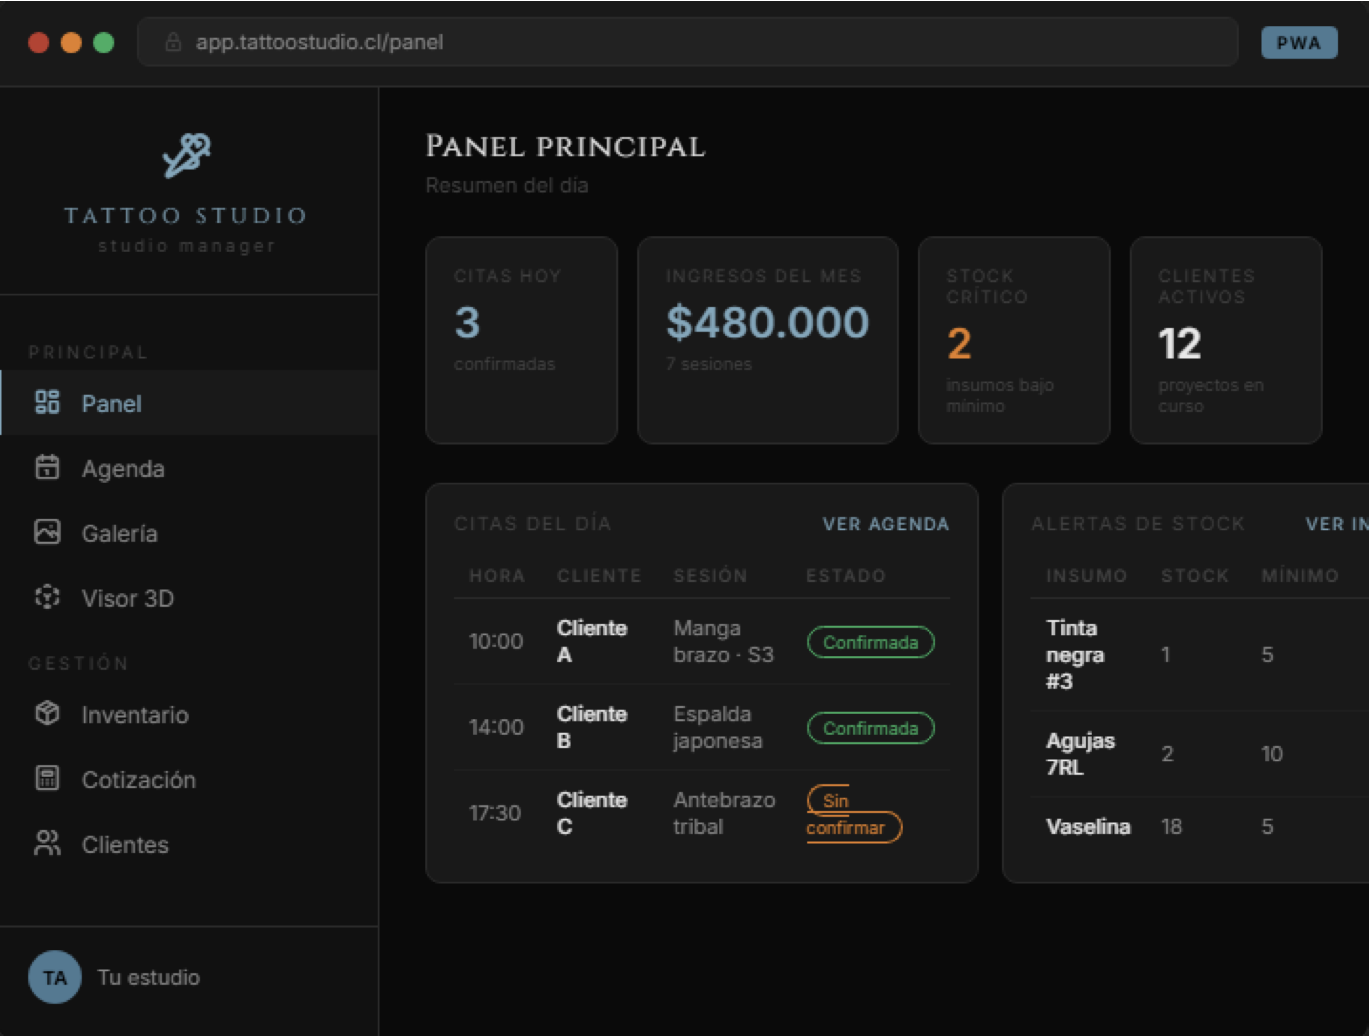
\includegraphics[width=0.8\textwidth]{fig-4-8-mockup-dashboard}
  \caption[Mockup Dashboard]{Mockup Dashboard.}
  \label{fig:mockupdashboard}
\end{figure}

\begin{figure}[H]
  \centering
  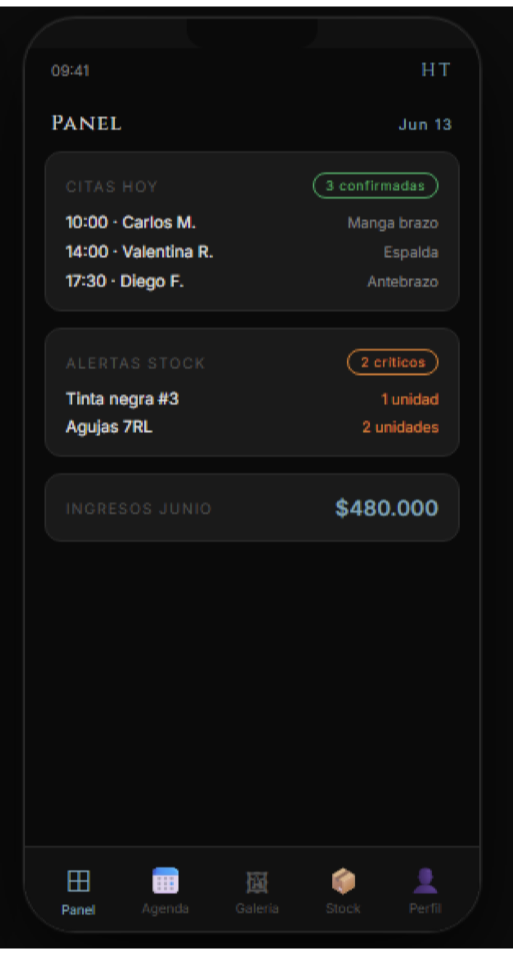
\includegraphics[width=0.3\textwidth]{fig-4-9-mockup-dashboard-movil}
  \caption[Mockup Dashboard Móvil]{Mockup Dashboard Móvil.}
  \label{fig:mockupdashboardmovil}
\end{figure}

La Figura \ref{fig:mockupdashboard} y \ref{fig:mockupdashboardmovil} muestran el diseño propuesto para el dashboard del sistema, tanto web como móvil, en el cual se muestran todos los componentes principales con lo que puede interactuar el usuario.

\begin{figure}[H]
  \centering
  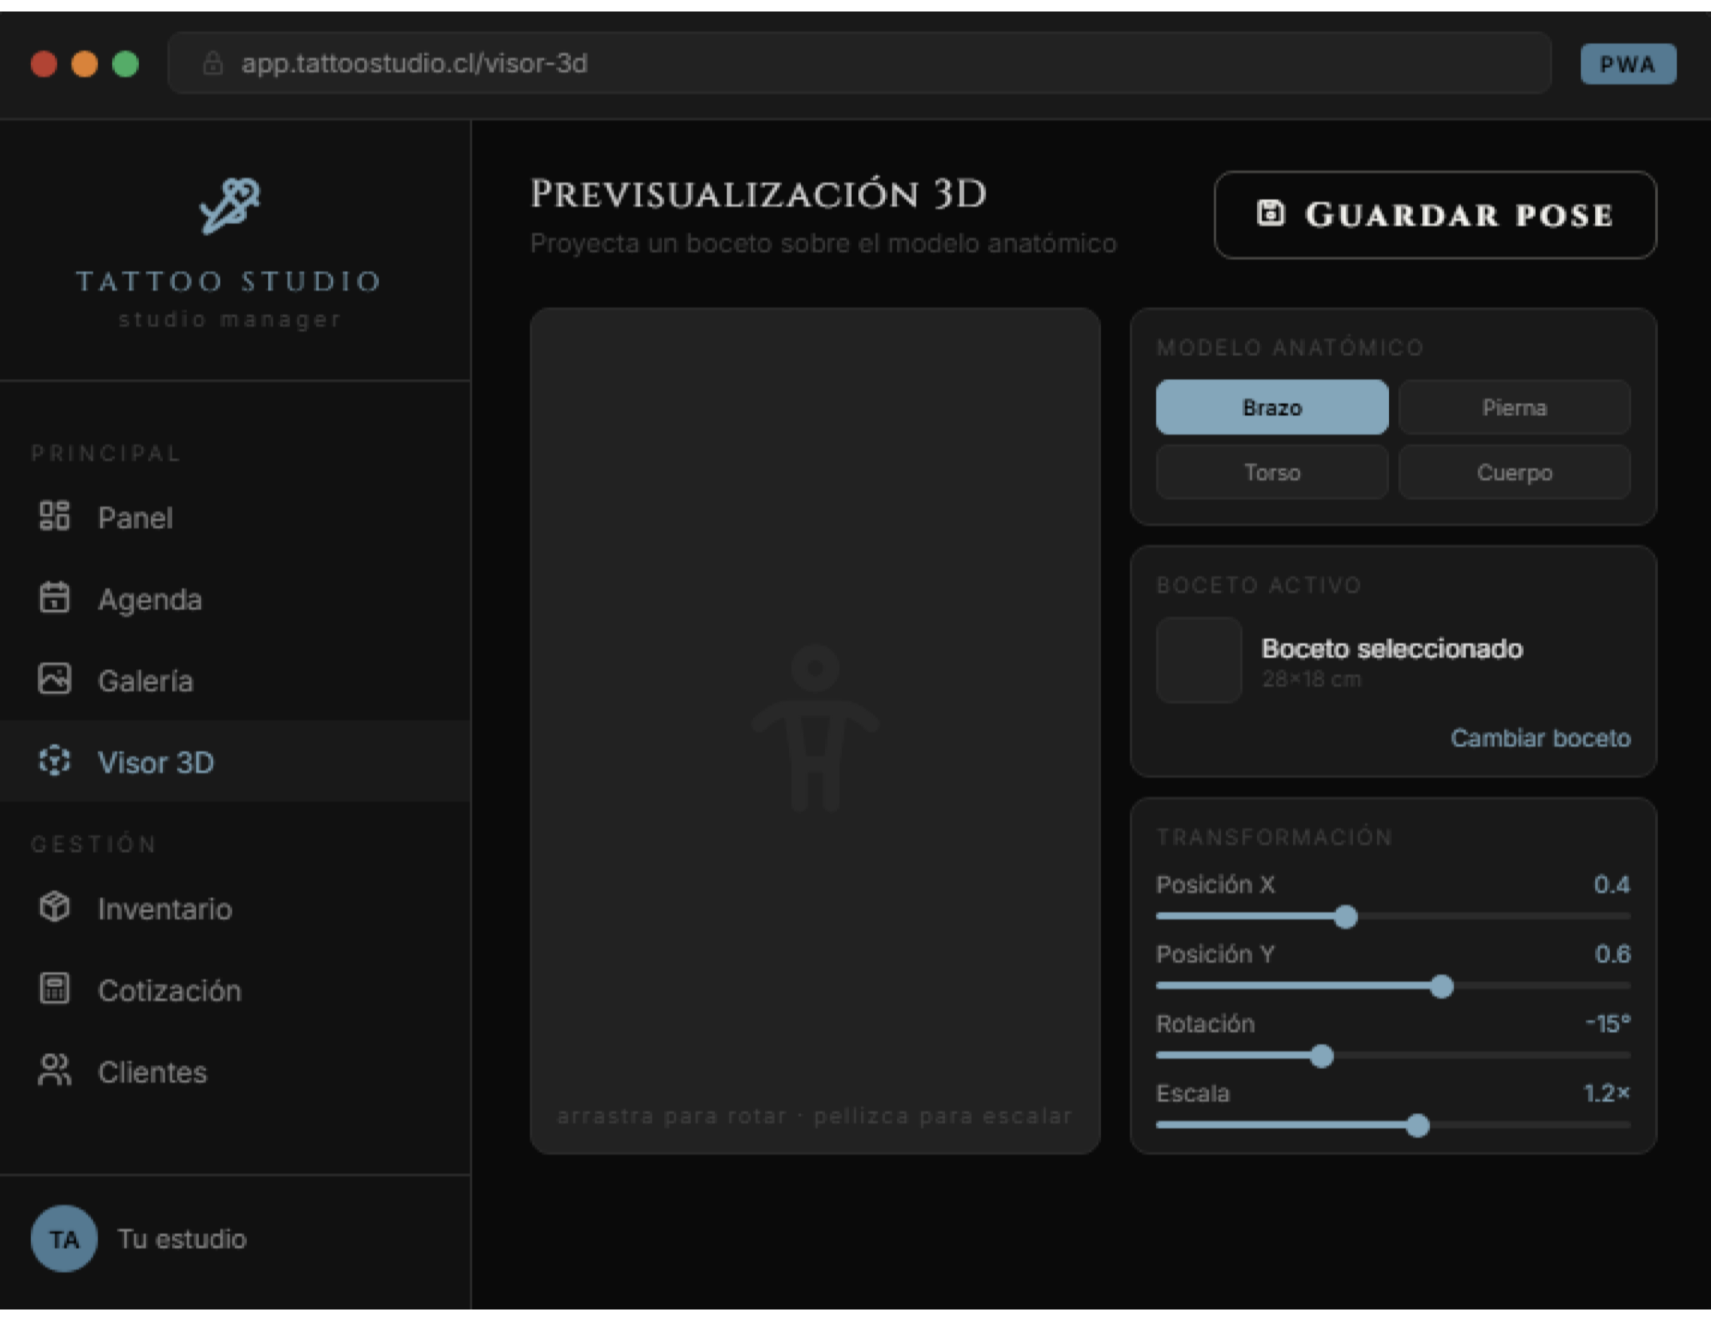
\includegraphics[width=\textwidth]{fig-4-10-mockup-previsualizacion-3d}
  \caption[Mockup Previsualización 3D]{Mockup Previsualización 3D.}
  \label{fig:mockup3d}
\end{figure}

\begin{figure}[H]
  \centering
  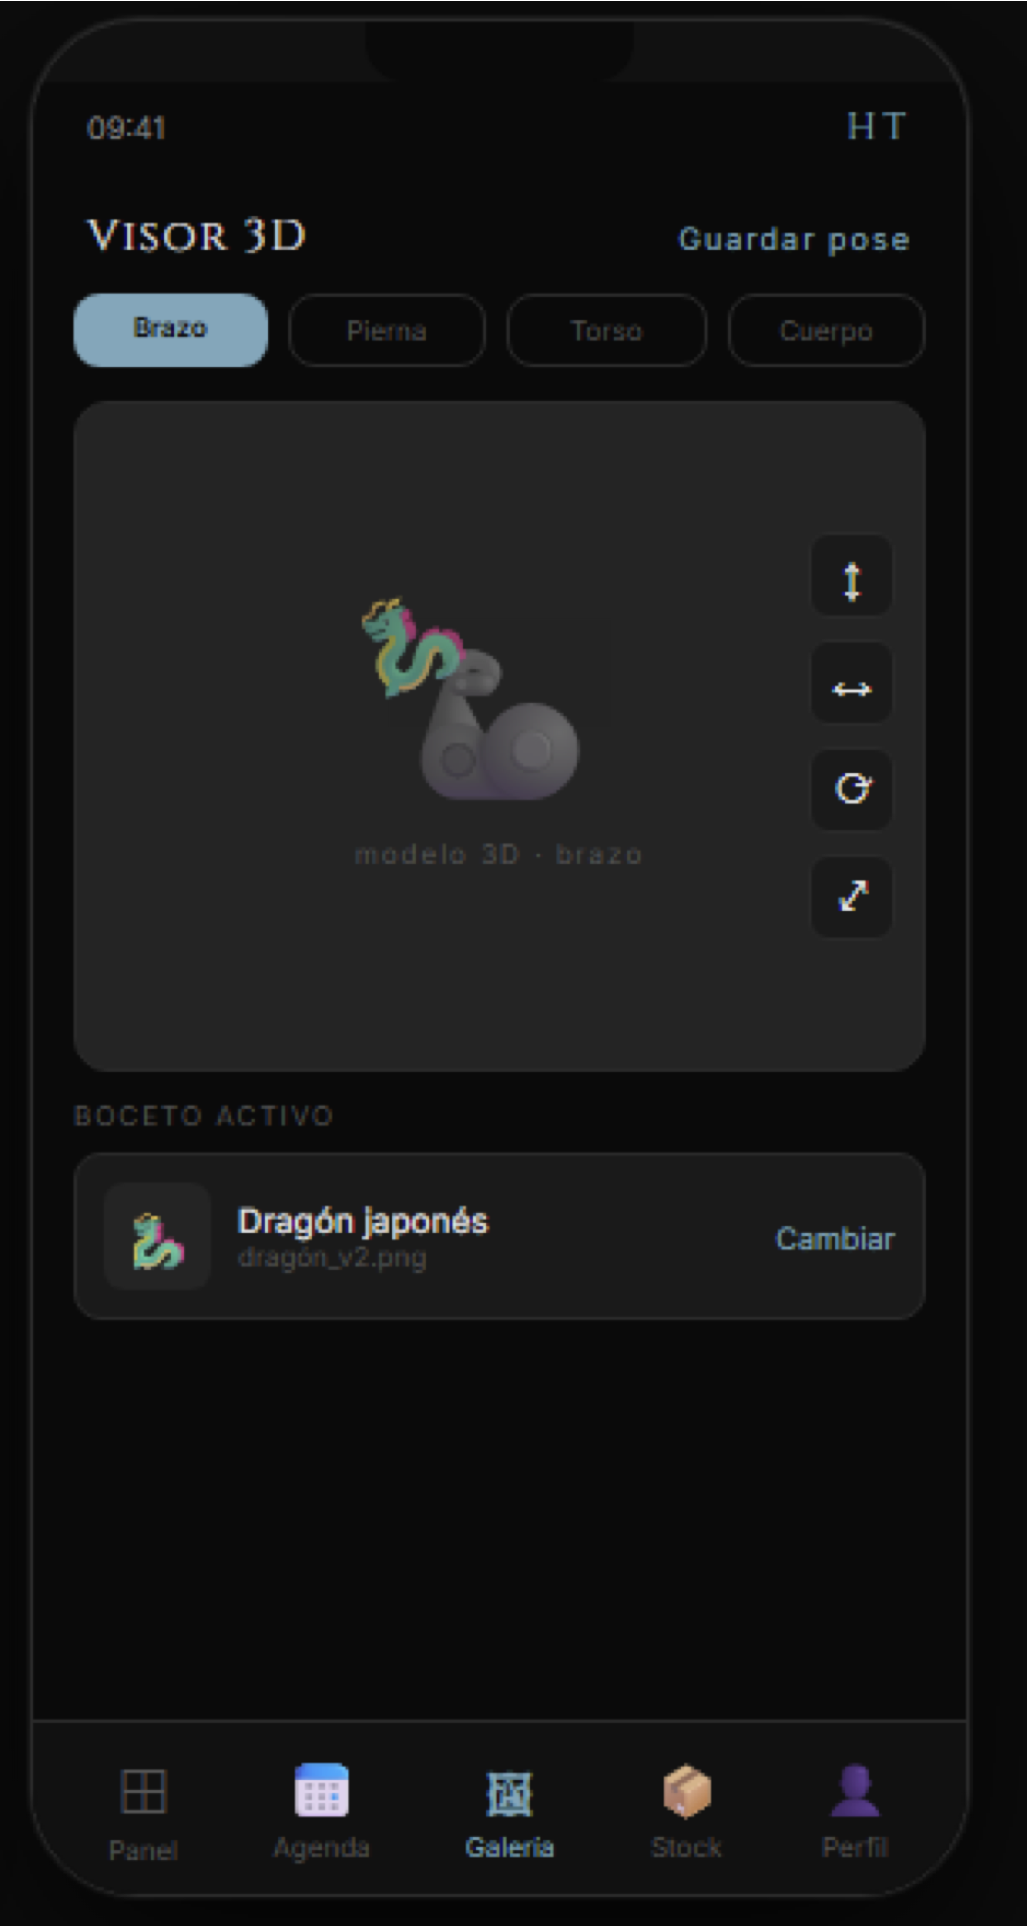
\includegraphics[width=0.6\textwidth]{fig-4-11-mockup-previsualizacion-3d-movil}
  \caption[Mockup Previsualización 3D Móvil]{Mockup Previsualización 3D Móvil.}
  \label{fig:mockup3dmovil}
\end{figure}

Por último, la Figura \ref{fig:mockup3d} y \ref{fig:mockup3dmovil} muestran el diseño propuesto para la vista de previsualización 3D, tanto web como móvil, en el cual se muestra la vista del modelo anatómico con el boceto proyectado sobre este, junto con las herramientas de ajuste para escalar, mover y rotar el diseño sobre el modelo 3D.

\section{Iteraciones}

A continuación, se detallan como se abordaron las iteraciones descritas en el Capítulo 3.1.2.

\subsection{Iteración 1}

En esta iteración, no existen historias de usuario asignadas, por lo que se enfocó en la planificación y diseño de la arquitectura del sistema, el modelo de datos y los mockups. Además, se establecieron las bases para el desarrollo de las siguientes iteraciones, definiendo los estándares de codificación, las herramientas a utilizar y la estructura general del proyecto.

\subsection{Iteración 2}

En esta iteración se comienza con la implementación de las historias de usuario HU01, HU02 y HU03, las cuales corresponden a la funcionalidad de autenticación. A continuación, se detalla la implementación siguiendo la metodología de desarrollo PXP.

\vspace{0.3cm}
\tituloparpegado{Inicio de Iteración}
En esta etapa, se crean y son registradas las tareas acordes a las historias de usuario, donde la Tabla \ref{tab:tareas} ilustra el registro de las tareas resultantes de la iteración.

\begin{table}[H]
  \centering
  \caption{Tareas asociadas a la Iteración 2}
  \label{tab:tareas}
  \renewcommand{\arraystretch}{1.2}
  \begin{tabular}{|l|l|p{8cm}|}
    \hline
    \textbf{Historia} & \textbf{Tarea} & \textbf{Descripción} \\
    \hline
    HU001 & T0001 & Crear diagrama de secuencia \\ \hline
    HU001 & T0002 & Crear ruta para inicio de sesión \\ \hline
    HU001 & T0003 & Crear vista para inicio de sesión \\ \hline
    HU002 & T0001 & Crear diagrama de secuencia \\ \hline
    HU002 & T0002 & Crear dashboard inicial \\ \hline
    HU002 & T0003 & Crear vista para cerrar sesión \\ \hline
    HU003 & T0001 & Crear diagrama de secuencia \\ \hline
    HU003 & T0002 & Crear ruta para olvidar contraseña \\ \hline
    HU003 & T0003 & Crear ruta para cambiar contraseña \\ \hline
    HU003 & T0004 & Crear vista para olvidar contraseña \\ \hline
    HU003 & T0005 & Crear vista para cambiar contraseña \\ \hline
    HU001, HU002, HU003 & T0009 & Creación y testeo de pruebas unitarias \\ \hline
    HU001, HU002, HU003 & T0010 & Creación y uso de sistema de pruebas \\ \hline
  \end{tabular}
\end{table}

\vspace{0.3cm}
\tituloparpegado{Diseño}
En esta etapa, se crean los diagramas de secuencia de las historias de usuario asociadas a la iteración. A continuación, las Figuras \ref{fig:seclogin}, \ref{fig:secdashboard} y \ref{fig:secolvido} ilustran el flujo de las principales funcioanlidades.

\begin{figure}[H]
  \centering
  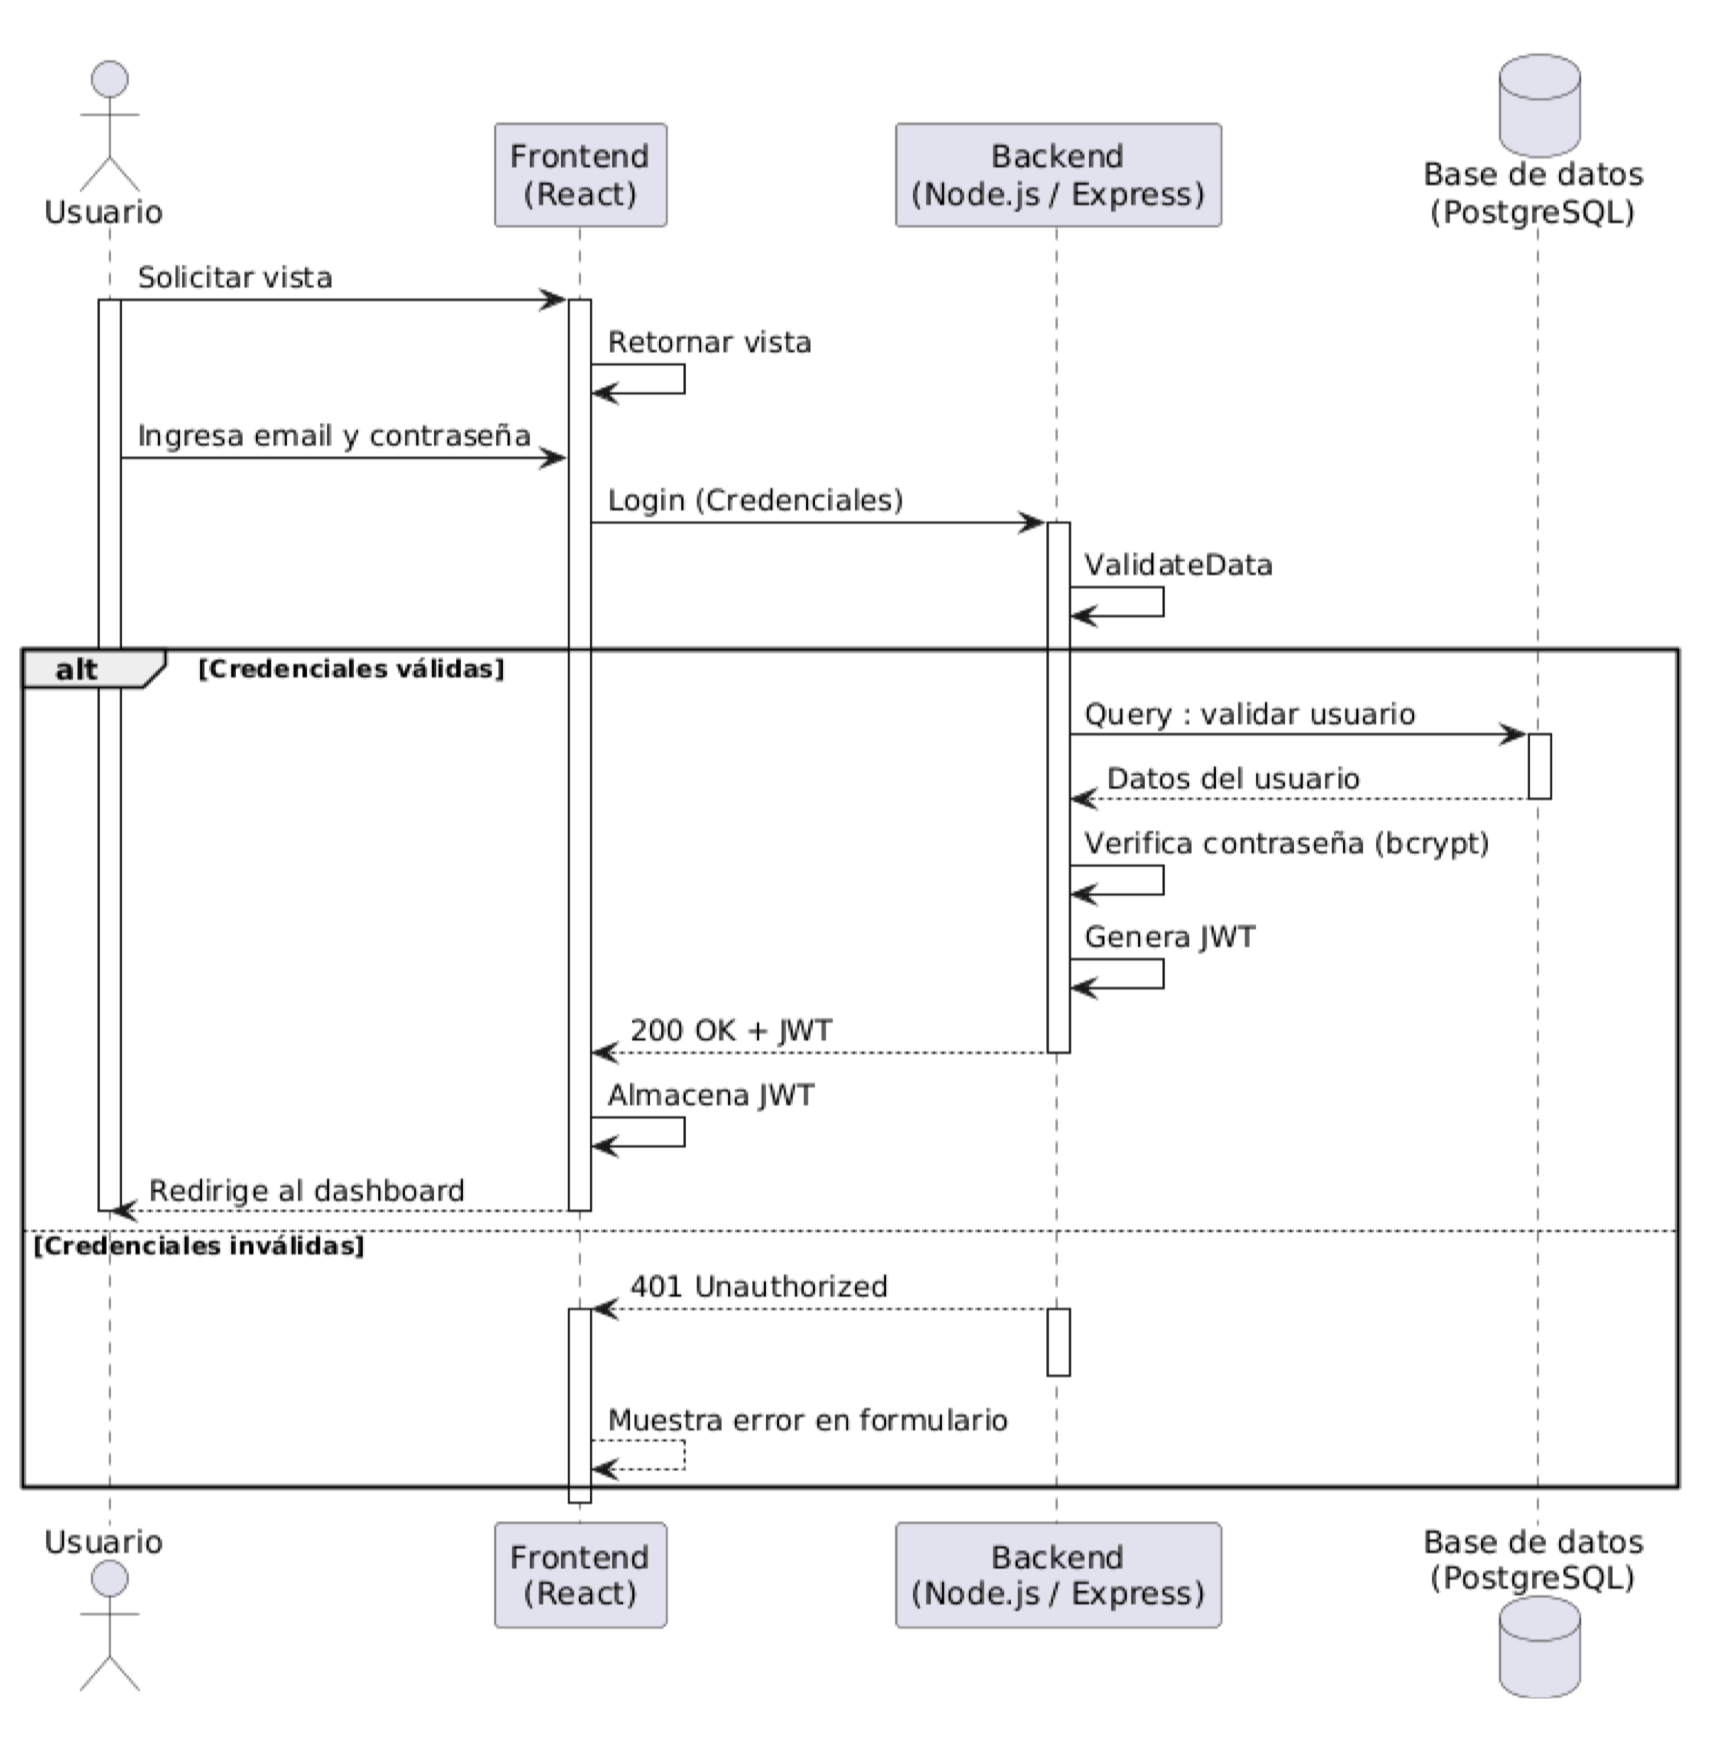
\includegraphics[width=\textwidth]{fig-4-12-secuencia-login}
  \caption[Diagrama de secuencia Inicio Sesión]{Diagrama de secuencia HU01: Login.}
  \label{fig:seclogin}
\end{figure}

\begin{figure}[H]
  \centering
  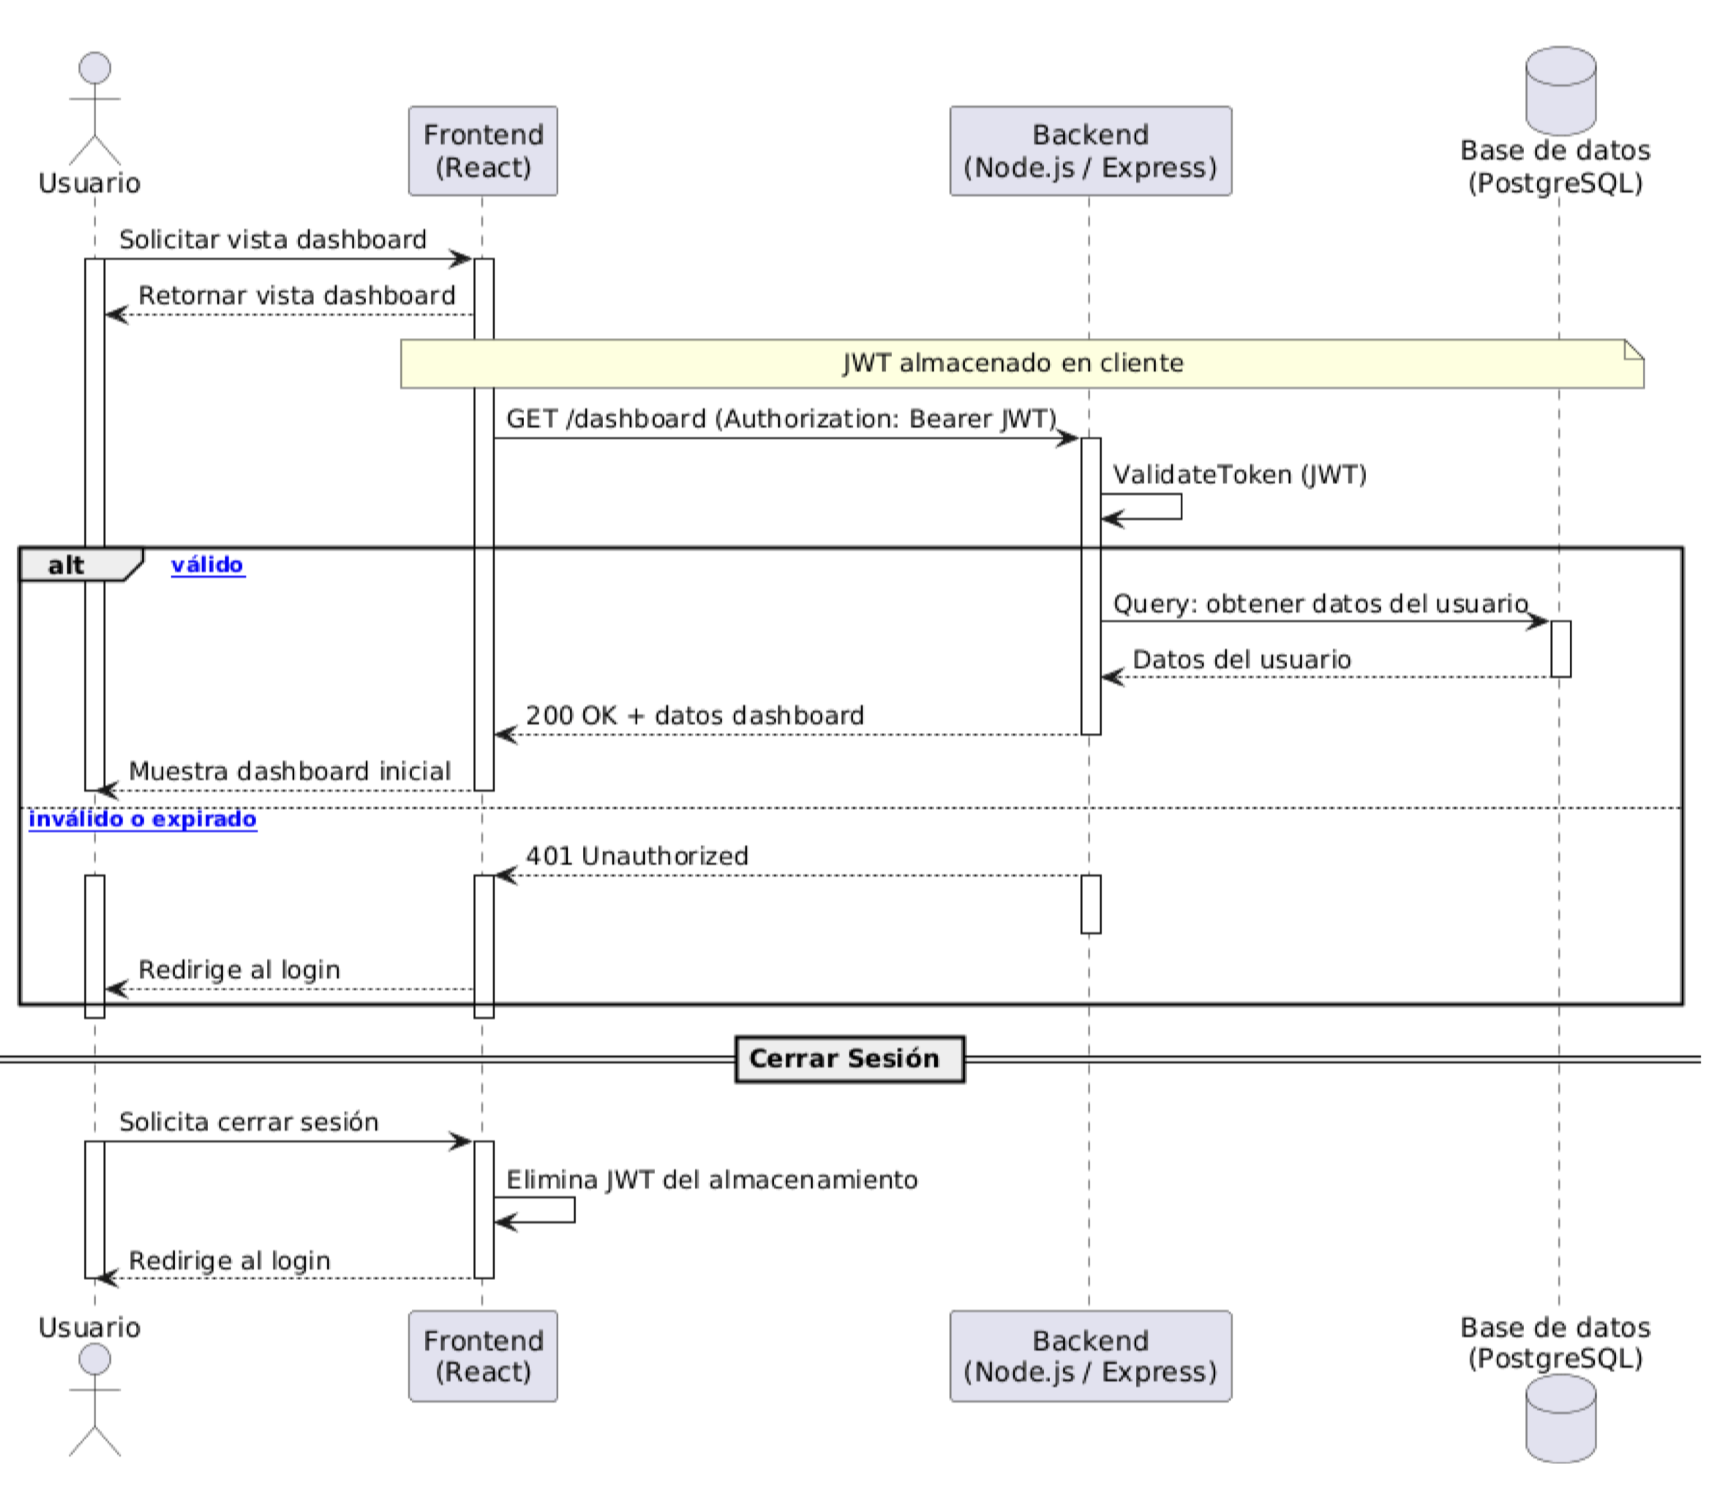
\includegraphics[width=\textwidth]{fig-4-13-secuencia-dashboard}
  \caption[Diagrama de secuencia Dashboard]{Diagrama de secuencia HU02: Dashboard.}
  \label{fig:secdashboard}
\end{figure}

\begin{figure}[H]
  \centering
  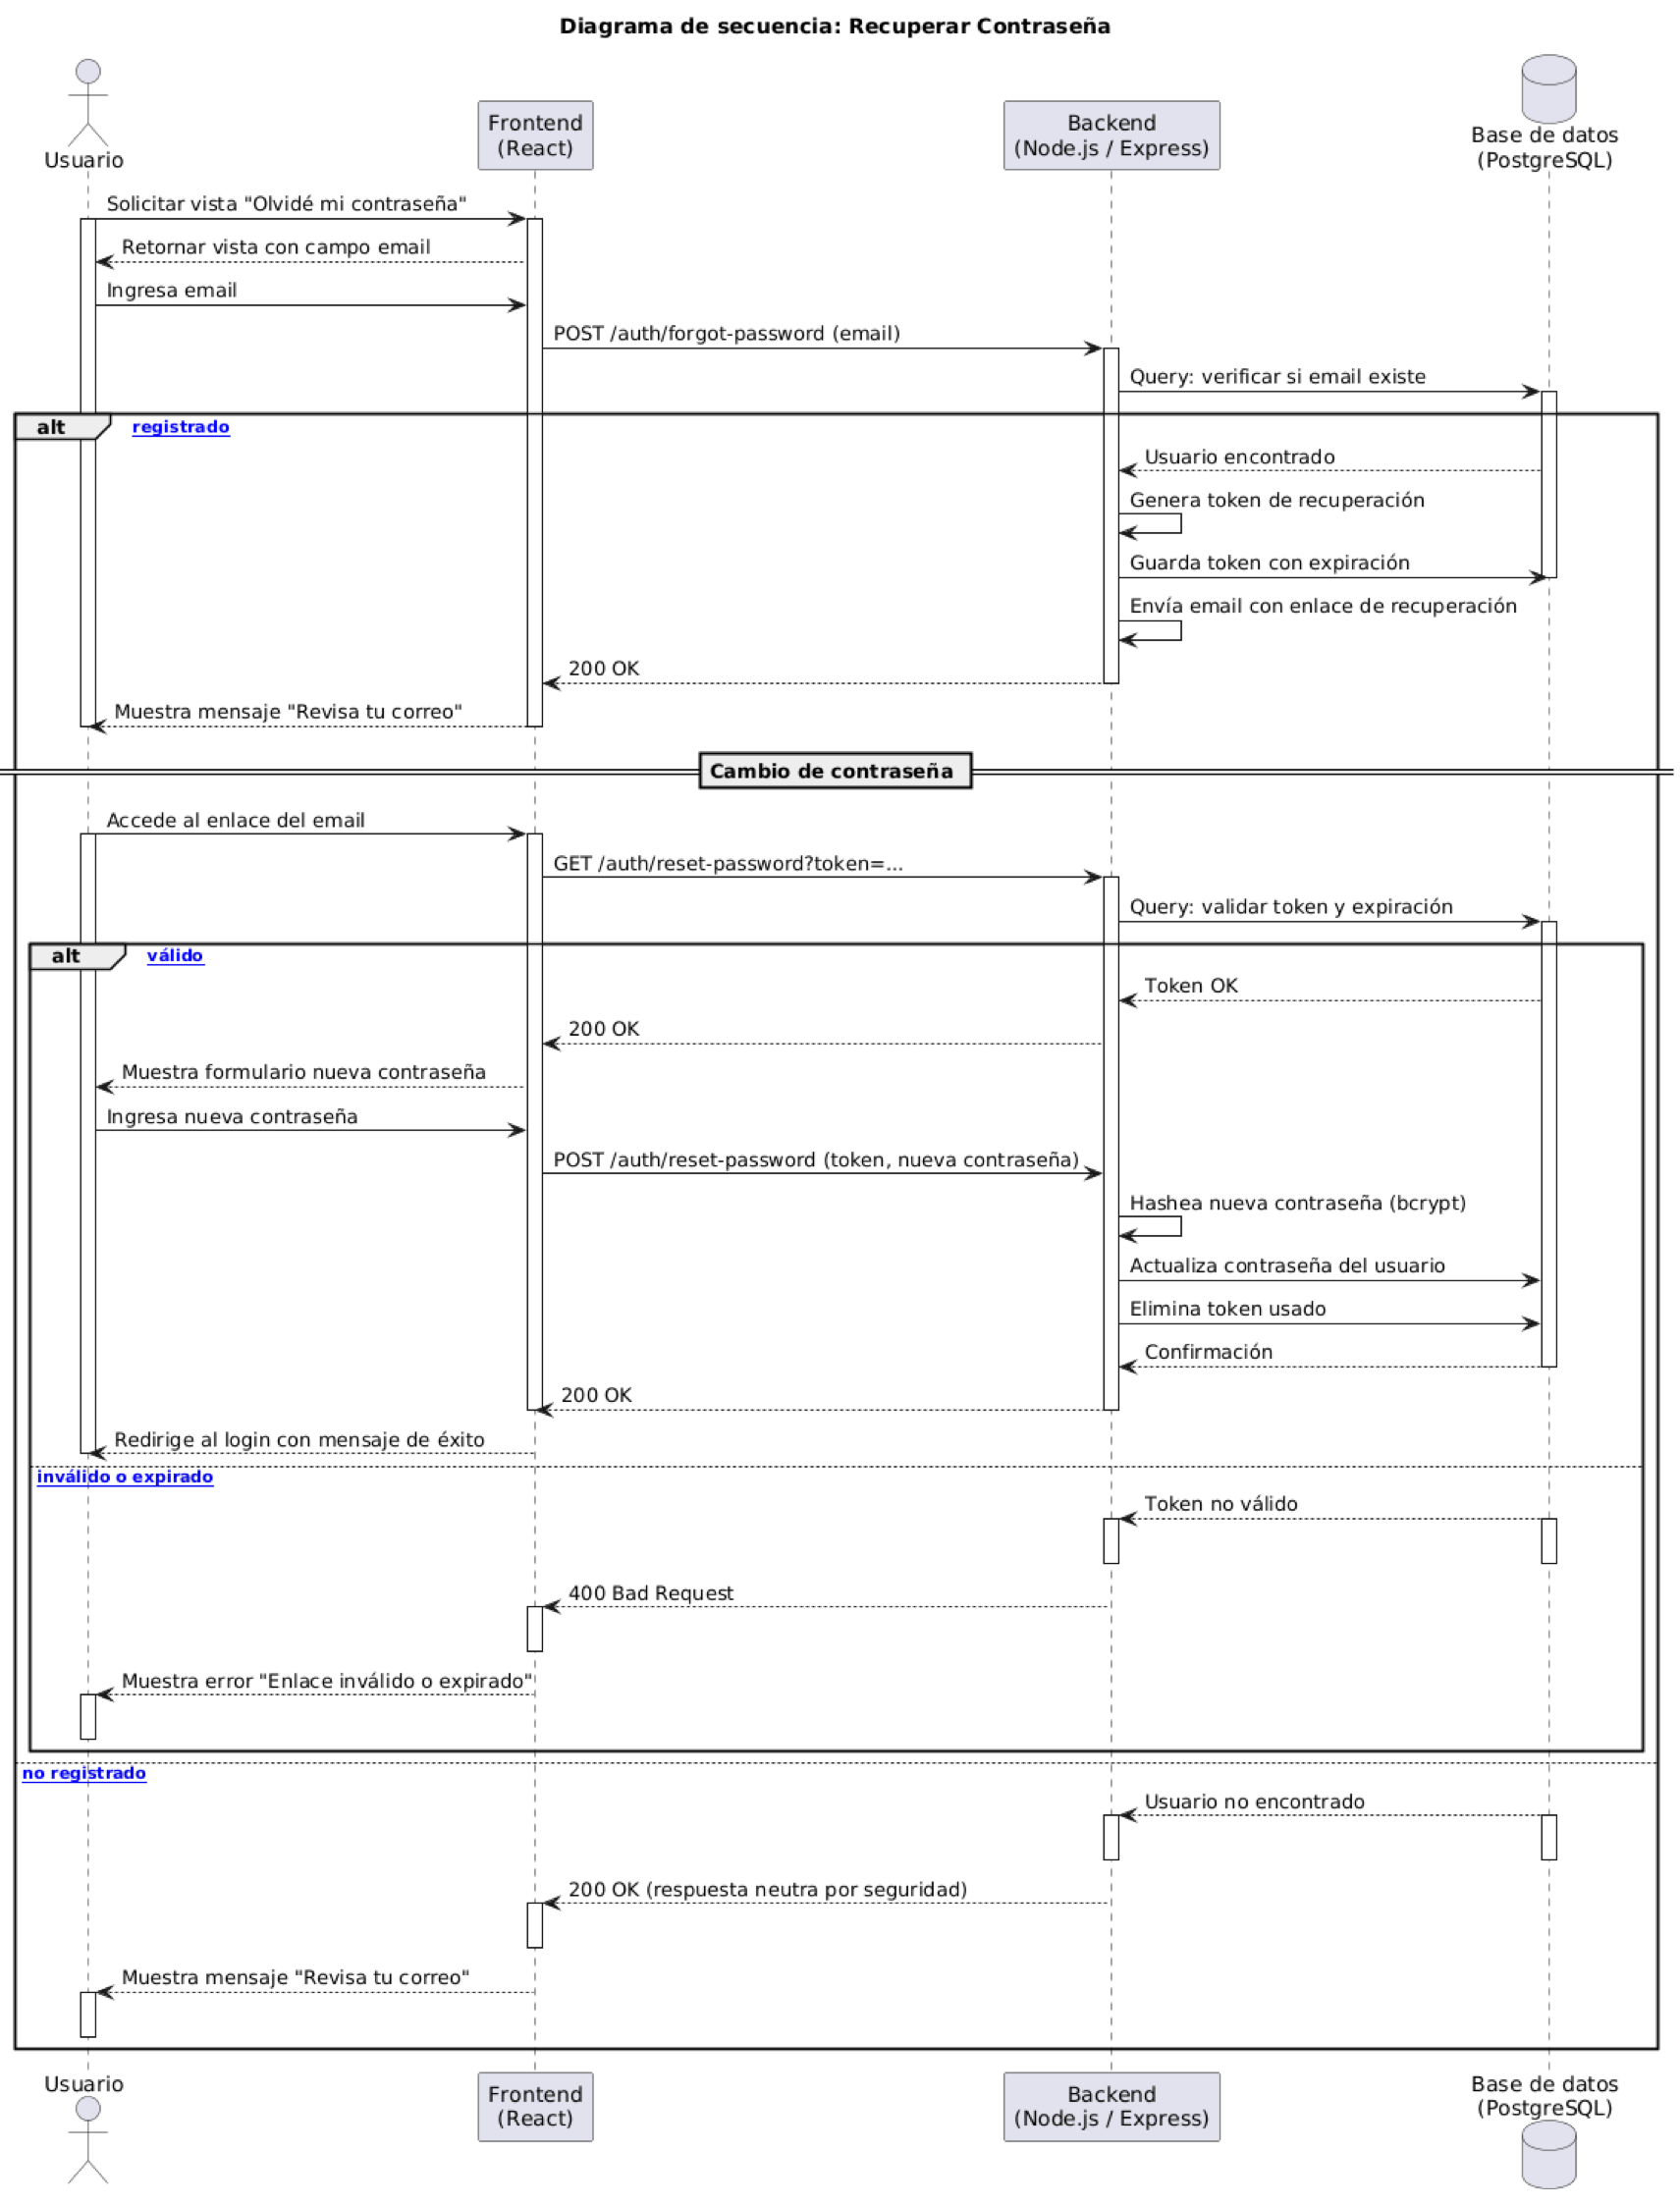
\includegraphics[width=\textwidth]{fig-4-14-secuencia-olvidar-contrasena}
  \caption[Diagrama de secuencia Olvidar Contraseña]{Diagrama de secuencia HU03: Olvidar Contraseña.}
  \label{fig:secolvido}
\end{figure}

\tituloparpegado{Implementación}
En esta etapa, se desarrolla tanto el backend como el frontend de las historias de usuario asignadas a la iteración. Se crean las rutas necesarias en el backend para manejar las solicitudes de inicio de sesión, cierre de sesión y recuperación de contraseña, mientras que en el frontend se desarrollan las vistas correspondientes para que el usuario pueda interactuar con estas funcionalidades. En el caso del inicio de sesión, se implemente JSON Web Tokens (JWT) para la autenticación y autorización de usuarios, asegurando acceso seguro a rutas protegidas del sistema. (Figura \ref{fig:jwt})

\begin{figure}[H]
  \centering
  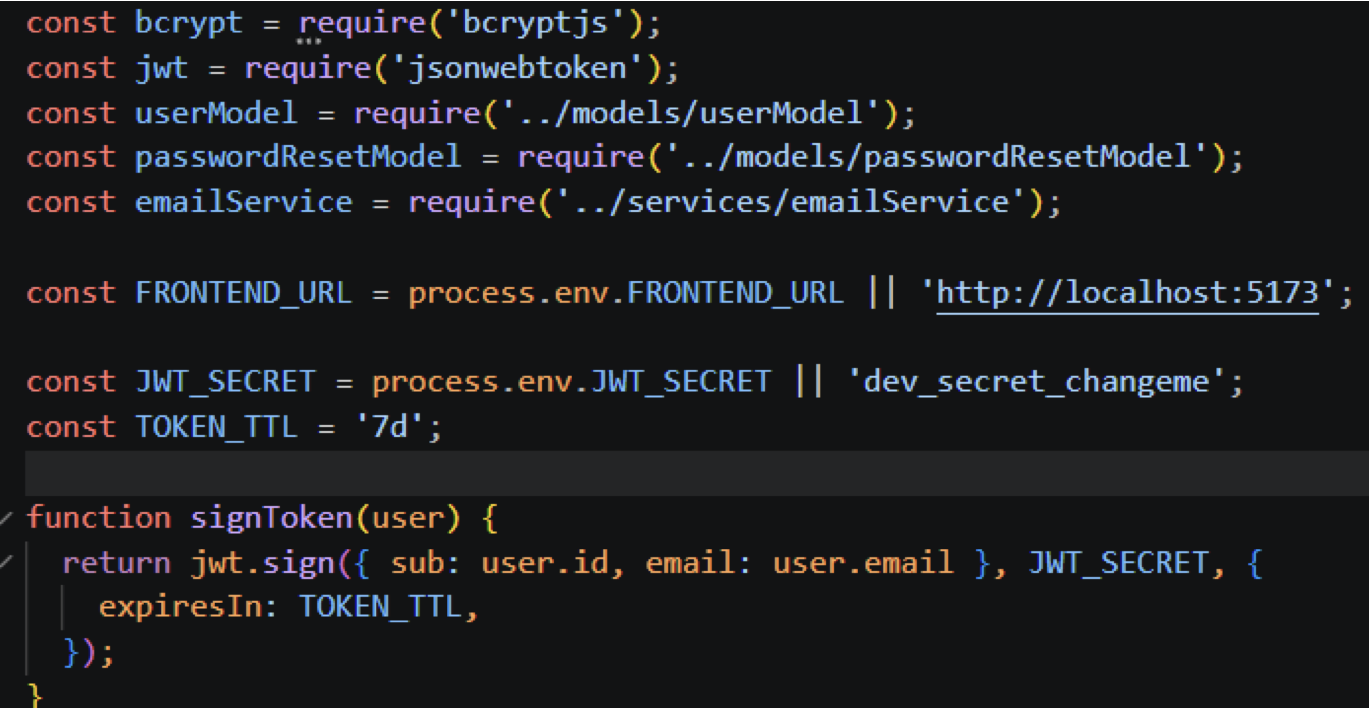
\includegraphics[width=0.8\textwidth]{fig-4-15-implementacion-jwt}
  \caption[Implementación JWT]{Implementación de autenticación mediante JSON Web Tokens (JWT).}
  \label{fig:jwt}
\end{figure}

Otro modulo que se implementó fue el servicio de envío de correos electrónicos para la funcionalidad de recuperación de contraseña, utilizando una librería de Node.js (Nodemailer) para enviar correos a través de un servicio SMTP, lo que permite a los usuarios recibir un enlace para restablecer su contraseña de manera segura como se puede ver en la Figura \ref{fig:email}.

\begin{figure}[H]
  \centering
  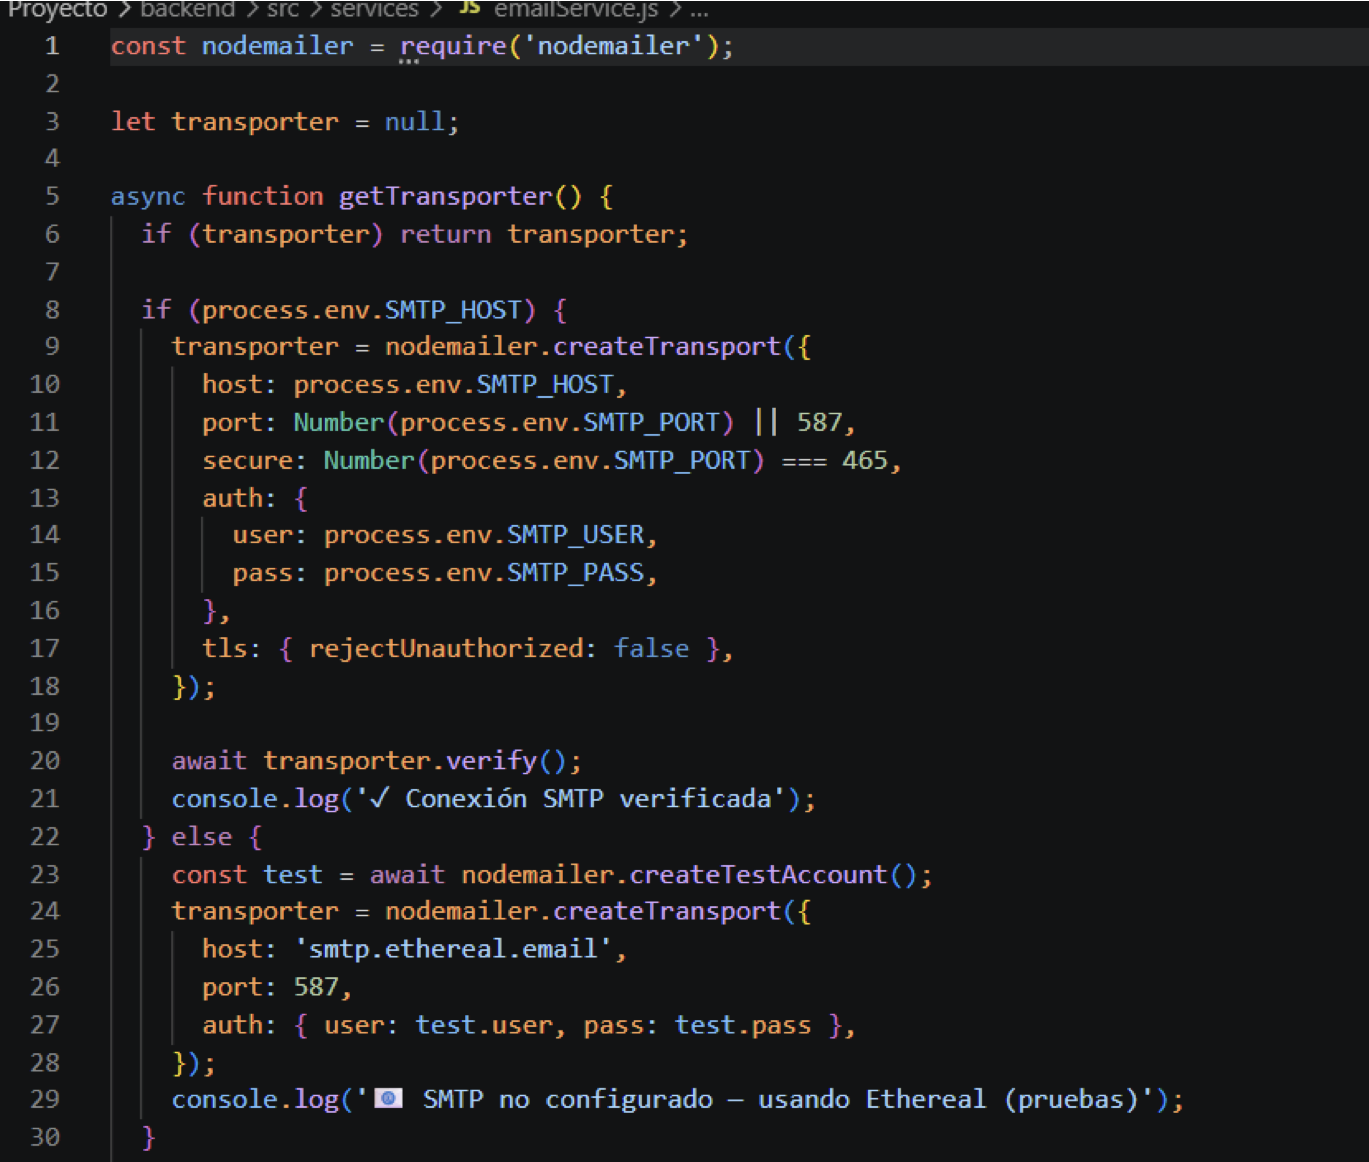
\includegraphics[width=0.8\textwidth]{fig-4-16-implementacion-email}
  \caption[Implementación Email]{Implementación del servicio de envío de correos electrónicos para recuperación de contraseña.}
  \label{fig:email}
\end{figure}

Al finalizar el desarrollo de las funcionalidades, se crean las pruebas unitarias correspondientes para cada una de las tareas definidas en el Inicio de Iteración, utilizando un framework de pruebas como Jest para asegurar que el código cumpla con los requisitos definidos en las historias de usuario \cite{jest}. La Figura \ref{fig:estructurapruebas} muestra la estrucutura de la prueba, donde se describe el test, usando supertest para simular las peticiones HTTP y verificar las respuestas del servidor. Los elementos claves para este ejemplo son post, que corresponde a la ruta a interactuar, send, que corresponde a los datos enviados en la petición, expect, que corresponde a las aserciones para validar el resultado esperado y end, que corresponde a condiciones.

\begin{figure}[H]
  \centering
  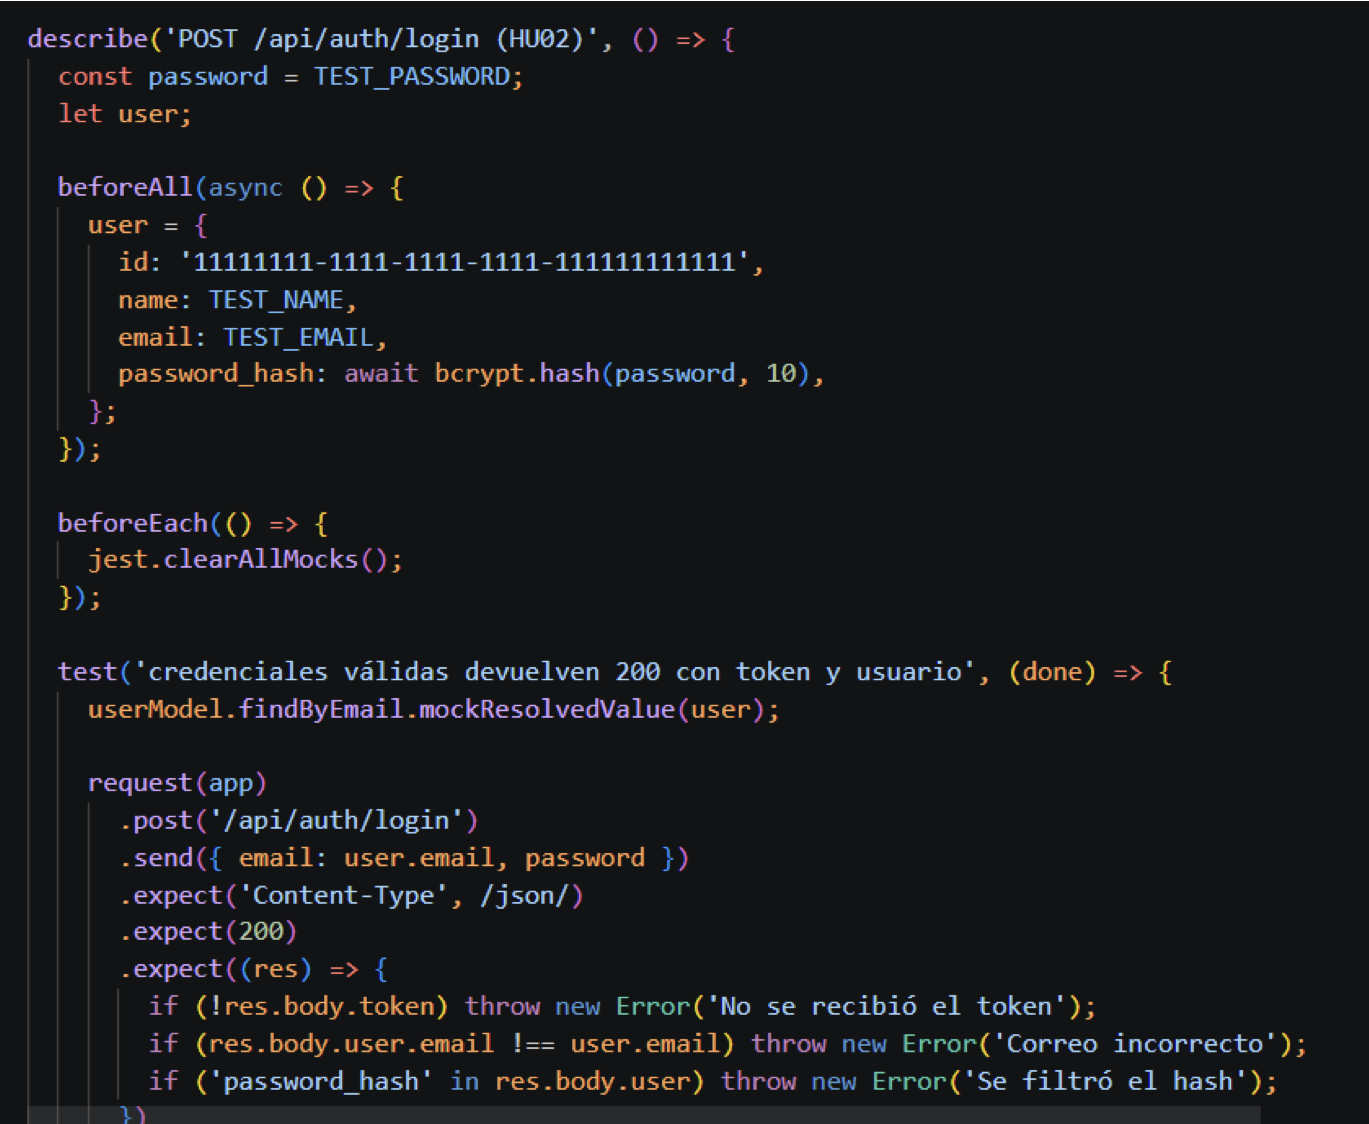
\includegraphics[width=0.8\textwidth]{fig-4-17-estructura-pruebas}
  \caption[Pruebas Unitarias]{Estructura de pruebas unitarias.}
  \label{fig:estructurapruebas}
\vspace{-5.72pt}
\end{figure}

La Figura \ref{fig:resultadopruebas} muestra los resultado de la ejecución de las pruebas unitarias.

\begin{figure}[h]
  \centering
  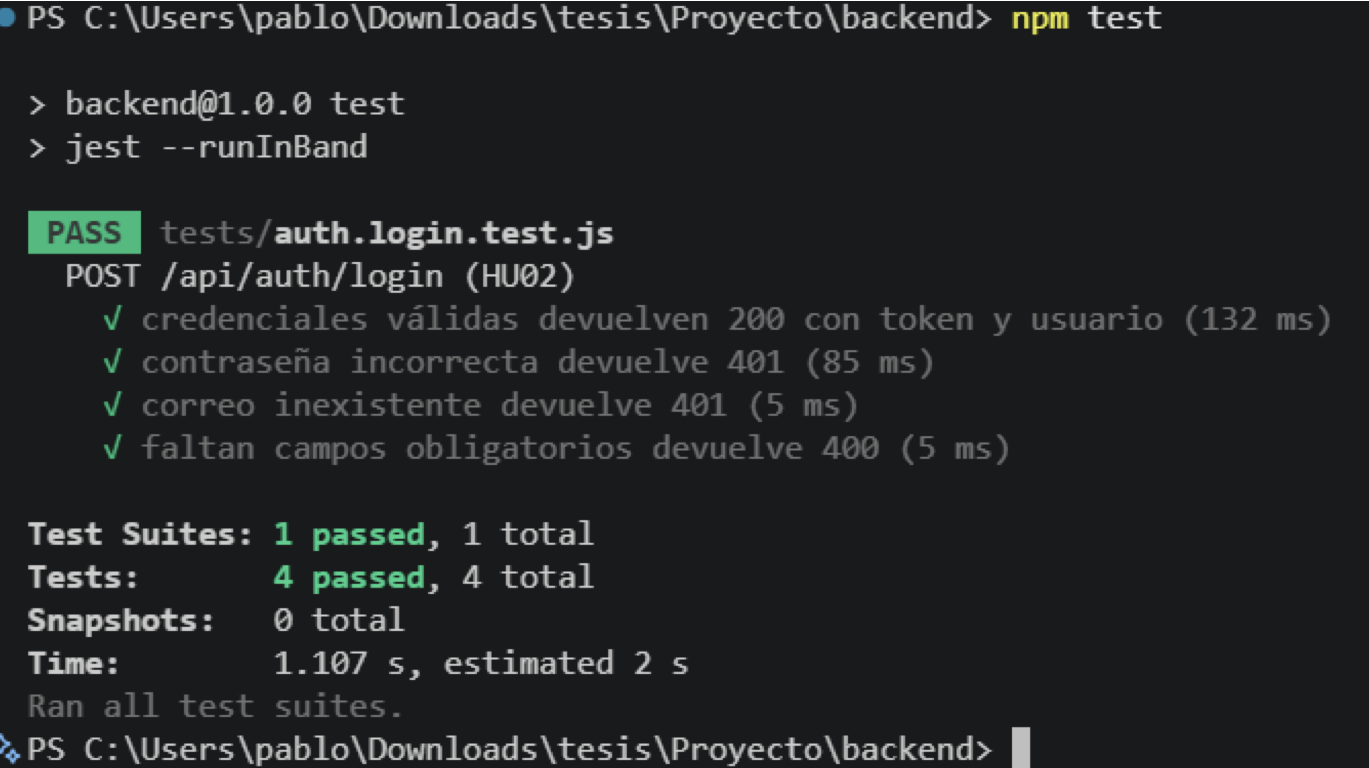
\includegraphics[width=0.8\textwidth]{fig-4-18-resultado-pruebas}
  \caption[Resultado Pruebas Unitarias]{Resultado de la ejecución de pruebas unitarias.}
  \label{fig:resultadopruebas}
\vspace{2.33pt}
\end{figure}

\tituloparpegado{Sistema de pruebas}
Después de la implementación, se lleva a cabo una fase de pruebas para esta iteración, evaluando los siguientes casos:

\begin{itemize}
  \item Ingresar con credenciales válidas.
  \item Ingresar a una ruta que no existe.
  \item Ingresar con un usuario que no existe.
  \item Ingresar con una contraseña incorrecta.
  \item Solicitar recuperación de contraseña con un correo registrado.
  \item Solicitar recuperación de contraseña con un correo no registrado.
  \item Solicitar recuperación de contraseña con un correo con formato inválido.
  \item Solicitar recuperación de contraseña sin ingresar un correo.
  \item Cerrar sesión correctamente.
\end{itemize}

\vspace{\parskip}
\tituloparpegado{Retrospectiva}
Al finalizar la iteración, se revisa si las estimaciones de tiempo para las historias de usuario fueron precisas y se identifican posibles mejoras en el proceso de desarrollo. En este caso, las estimaciones fueron acertadas, y se completaron todas las funcioanlidades planeadas sin pendientes.

\chapter*{Glosario}
\addcontentsline{toc}{chapter}{Glosario}
\markboth{GLOSARIO}{GLOSARIO}

\begin{description}
  \item \textbf{Framework:} Un framework es un conjunto de herramientas, bibliotecas y convenciones que proporcionan una estructura predefinida para el desarrollo de aplicaciones. Facilita la organización del código, la reutilización de componentes y la implementación de funcionalidades comunes, permitiendo a los desarrolladores centrarse en la lógica específica de su aplicación en lugar de preocuparse por detalles de bajo nivel.

  \item \textbf{JWT (JSON Web Token):} Es un estándar abierto (RFC 7519) que define un formato compacto y seguro para la transmisión de información entre partes como un objeto JSON. Se utiliza comúnmente para la autenticación y autorización en aplicaciones web, permitiendo a los servidores generar tokens que contienen información del usuario y sus permisos, los cuales pueden ser verificados y decodificados por el cliente para acceder a recursos protegidos.

  \item \textbf{Nodemailer:} Es una biblioteca de Node.js que facilita el envío de correos electrónicos desde aplicaciones Node.js. Proporciona una interfaz sencilla para configurar y enviar correos electrónicos utilizando diversos servicios de correo, como SMTP, Gmail, Outlook, entre otros

  \item \textbf{Supertest:} Es una biblioteca de pruebas para Node.js que permite realizar pruebas de integración en aplicaciones web. Proporciona una API fácil de usar para simular solicitudes HTTP y verificar las respuestas del servidor, lo que facilita la validación de rutas, controladores y middleware en aplicaciones Express u otros frameworks web.

  \item \textbf{Jest:} Es un framework de pruebas de JavaScript desarrollado por Facebook, diseñado para trabajar con proyectos que utilizan React, aunque también es compatible con otros entornos JavaScript. Jest proporciona una experiencia de prueba completa con características como pruebas unitarias, pruebas de integración, pruebas de extremo a extremo, y una interfaz de usuario amigable.

  \item \textbf{API:} Una API (Interfaz de Programación de Aplicaciones) es un conjunto de reglas y protocolos que permiten la comunicación entre diferentes software. Las APIs definen cómo los componentes de software deben interactuar, permitiendo a los desarrolladores acceder a funcionalidades específicas de una aplicación o servicio sin necesidad de conocer su implementación interna.

  \item \textbf{SMTP (Simple Mail Transfer Protocol):} Es un protocolo de comunicación utilizado para el envío de correos electrónicos a través de Internet. SMTP define las reglas y procedimientos para la transferencia de mensajes de correo electrónico entre servidores de correo, permitiendo a los usuarios enviar correos electrónicos desde sus clientes de correo electrónico a los servidores de correo y entre servidores de correo.

  \item \textbf{GitHub:} Es una plataforma de desarrollo colaborativo que utiliza el sistema de control de versiones Git. GitHub permite a los desarrolladores alojar, compartir y colaborar en proyectos de software, facilitando la gestión de código fuente, el seguimiento de cambios, la revisión de código y la integración continua.
\end{description}


\printbibliography[heading=bibintoc]

\end{document}
